\documentclass[12pt,a4paper]{report}

% --- Packages ---
\usepackage{fontspec}
\usepackage[english]{babel}
\usepackage{geometry}
\geometry{margin=2.5cm}
\usepackage{setspace}
\onehalfspacing
\usepackage{graphicx}
\usepackage{float}
\usepackage{hyperref}
\hypersetup{colorlinks=true, linkcolor=black, urlcolor=blue, citecolor=black}
\usepackage{listings}
\usepackage{xcolor}
\usepackage{booktabs}
\usepackage{longtable}
\usepackage{array}
\usepackage{enumitem}
\usepackage{titlesec}
\usepackage{fancyhdr}
\usepackage{tocbibind}
\usepackage{caption}
\usepackage{amsmath}
\usepackage{tikz}
\usetikzlibrary{matrix,positioning,arrows.meta,fit,backgrounds}

% --- Page style ---
\pagestyle{fancy}
\fancyhf{}
\rhead{\thepage}
\lhead{Opic: A Topic-Structured Learning Platform with User-Driven Content Personalisation}
\cfoot{}

% --- Code listing style ---
\lstdefinestyle{code}{
  backgroundcolor=\color{gray!10},
  basicstyle=\ttfamily\footnotesize,
  breaklines=true,
  frame=single,
  numbers=left,
  numberstyle=\tiny\color{gray},
  keywordstyle=\color{blue},
  commentstyle=\color{green!60!black},
  stringstyle=\color{orange},
}
\lstset{style=code}

% Helper for missing figures
\newcommand{\missingfig}[2]{%
  \begin{center}
    \fbox{\parbox{0.7\textwidth}{\centering\vspace{1.5cm}%
      \textit{[Figure placeholder: #1]}\\[0.3cm]%
      \small #2\vspace{1.5cm}}}%
  \end{center}%
}

\date{June 2026}

\begin{document}

% ============================================================
% TITLE PAGE
% ============================================================

\begin{titlepage}
\centering
\thispagestyle{empty}

\textbf{\large UNIVERSITY OF SCIENCE AND TECHNOLOGY OF HANOI}\\[0.3cm]
\textbf{\large DEPARTMENT OF INFORMATION AND COMMUNICATION TECHNOLOGY}\\[1.5cm]

\IfFileExists{logo.png}{%
  
\includegraphics[width=7cm]{logo.png}%
}{%
  \fbox{\parbox{4cm}{\centering\vspace{1cm}\small[University Logo]\vspace{1cm}}}%
}\\[1.5cm]

{\LARGE \textbf{BACHELOR THESIS}}\\[1.2cm]

\noindent\rule{\textwidth}{0.8pt}\\[1.2cm]

{\fontsize{22}{28}\selectfont \textbf{A Topic-Structured Learning Platform\\[0.4cm]
with User-Driven Content Personalisation}}\\[1.2cm]

\noindent\rule{\textwidth}{0.8pt}\\[2.0cm]

\begin{center}
\begin{tabular}{r@{\quad}l}
\textit{Student:}             & \textbf{Vũ Tùng Lâm} \\[0.5cm]
\textit{Student ID:}          & \textbf{22BI13241} \\[0.5cm]
\textit{External Supervisor:} & \textbf{Trương Trọng Tuấn} \\[0.25cm]
\textit{Internal Supervisor:} & \textbf{Nguyễn Thị Hà Trang} \\
\end{tabular}
\end{center}

\vfill
{\large \textbf{Hanoi, June 2026}}
\end{titlepage}

% ============================================================
% CERTIFICATION PAGE (page 2)
% ============================================================
\newpage
\thispagestyle{empty}
\vspace*{3cm}

\noindent To whom it may concern,

\vspace{1cm}

\noindent I, \textbf{Trương Trọng Tuấn}, certify that the thesis of Mr \textbf{Vũ Tùng Lâm} is qualified to be presented in the Internship Jury 2026--2027.

\vspace{5cm}

\begin{flushright}
Hanoi, 29\textsuperscript{th} June 2026

\vspace{2cm}

\textbf{Supervisor's signature}
\end{flushright}

\newpage
\chapter*{Acknowledgements}
\addcontentsline{toc}{chapter}{Acknowledgements}

I would like to thank my supervisors for their guidance and feedback throughout this project. I also want to thank my classmates who took the time to test the platform -- their bug reports were genuinely useful and caught things I had missed. And thank you to my family for putting up with me during the long stretches of late-night coding.

\newpage

% ============================================================
% ABSTRACT
% ============================================================
\chapter*{Abstract}
\addcontentsline{toc}{chapter}{Abstract}

Finding good learning material online is easy. Knowing what to study first, what order makes sense, and which of the thousands of results are actually useful -- that is the harder problem. Opic was built to address this for university students, particularly in ICT, Data Science, and BIT programmes.

The platform organises content into topic roadmaps with prerequisite links, lets users submit and rate resources, and uses a recommendation engine to suggest relevant materials based on each user's behaviour. Technically, it is a React frontend talking to a FastAPI backend over a REST API, with a PostgreSQL database. The recommender uses user-based collaborative filtering (UBCF) with cosine similarity and a Bayesian average to handle sparse ratings. For new users with no history, an onboarding quiz seeds the cold-start fallback. When marking a topic complete, users take a short Gemini-generated quiz; getting three or more wrong sends them back to review first.

The system is deployed on Render (backend) and Vercel (frontend) and was tested end-to-end with multiple accounts. All fifteen functional requirements are working on the live deployment.

\textbf{Keywords:} recommender systems, collaborative filtering, learning platform, FastAPI, React, cold-start, Bayesian average, knowledge quiz

\newpage

% ============================================================
% TABLE OF CONTENTS
% ============================================================
\tableofcontents
\newpage

% ============================================================
% LIST OF FIGURES
% ============================================================
\listoffigures
\newpage

% ============================================================
% LIST OF TABLES
% ============================================================
\listoftables
\newpage

% ============================================================
% LIST OF ABBREVIATIONS
% ============================================================
\chapter*{List of Abbreviations}
\addcontentsline{toc}{chapter}{List of Abbreviations}

\begin{longtable}{p{0.2\textwidth} p{0.7\textwidth}}
\toprule
\textbf{Abbreviation} & \textbf{Full Form} \\
\midrule
\endfirsthead
\toprule
\textbf{Abbreviation} & \textbf{Full Form} \\
\midrule
\endhead
API   & Application Programming Interface \\
BCrypt & Blowfish Crypt -- password hashing algorithm \\
CDN   & Content Delivery Network \\
CF    & Collaborative Filtering \\
CI/CD & Continuous Integration / Continuous Delivery \\
CORS  & Cross-Origin Resource Sharing \\
DS    & Data Science \\
ERD   & Entity-Relationship Diagram \\
FR    & Functional Requirement \\
HTTP  & Hypertext Transfer Protocol \\
HTTPS & Hypertext Transfer Protocol Secure \\
ICT   & Information and Communication Technology \\
JWT   & JSON Web Token \\
JSON  & JavaScript Object Notation \\
LLM   & Large Language Model \\
MCQ   & Multiple Choice Question \\
NFR   & Non-Functional Requirement \\
ORM   & Object-Relational Mapper \\
REST  & Representational State Transfer \\
SPA   & Single-Page Application \\
SQL   & Structured Query Language \\
SMTP  & Simple Mail Transfer Protocol \\
TLS   & Transport Layer Security \\
UC    & Use Case \\
UBCF  & User-Based Collaborative Filtering \\
UI    & User Interface \\
URL   & Uniform Resource Locator \\
USTH  & University of Science and Technology of Hanoi \\
\bottomrule
\end{longtable}

\newpage

% ============================================================
% CHAPTER 1 -- INTRODUCTION
% ============================================================
\chapter{Introduction}

\section{Context and Motivation}

There is no shortage of learning material online. YouTube, Coursera, and Medium alone publish thousands of tutorials, articles, and videos every week \cite{coursera2023}. For a student trying to pick up a new topic -- say, data structures or web development -- the actual problem is not finding content. It is figuring out what to study first, what order makes sense, and which of the hundred results that come up are actually worth the time.

This problem has been studied in the e-learning literature. Drachsler and Greller \cite{drachsler2016} call it the ``paradox of choice'': more resources does not mean better learning, and too many options can increase cognitive load and leave learners more confused than when they started. Burke \cite{burke2002} made a similar point -- web-based learning environments have long struggled to show people content that is relevant to them specifically, rather than just popular in general.

Recommender systems have been one answer to this since the mid-1990s, starting with the GroupLens project \cite{resnick1994}, which applied collaborative filtering to Usenet articles. Collaborative filtering has since become the standard approach for personalised recommendation \cite{koren2009} and is used by Netflix, Spotify, and Amazon at scale. Its use in education, however, is less developed -- most academic platforms still depend on manually curated course structures \cite{tang2015}.

Opic was built to address this gap. The name comes from \textit{topic}, the core unit of learning in the system. It is a web-based platform that organises content into structured topic roadmaps, lets users submit and rate resources, and uses a recommendation engine to surface materials relevant to each person based on how they interact with the platform.

The target audience is university students, particularly in ICT, Data Science, and BIT programmes at USTH, where students are expected to do a lot of self-directed study and the volume of available material can be hard to navigate \cite{zimmerman2002,brusilovsky2007}.

\section{Objectives}

This project set out to build a working, deployable learning platform that tackles three specific problems students face:

\begin{enumerate}
  \item \textbf{Navigation} -- not knowing what to study or in what order.
  \item \textbf{Quality} -- not knowing which resources are actually good.
  \item \textbf{Personalisation} -- getting the same results as everyone else regardless of background.
\end{enumerate}

These are addressed through topic roadmaps with prerequisite links, a community submission and admin review pipeline, and a user-based collaborative filtering engine. UBCF was chosen over content-based filtering (which needs expert tagging) and matrix factorisation (which requires offline training) because it is simpler, interpretable, and works on live data \cite{herlocker2004}. The cold-start problem for new users with no history is handled through an onboarding quiz \cite{schein2002}.

\section{Expected Outcome}

By the end of the project, the following were working and deployed:

\begin{itemize}
  \item A live web application where users can register, take the onboarding quiz, browse topic roadmaps, and access curated resources.
  \item A recommendation engine that gives useful suggestions from day one (via the onboarding quiz cold-start) and gets better as users rate and complete resources.
  \item An admin content pipeline: users submit resources, admins approve or reject them, and only approved resources appear on topic pages.
  \item Topic-level progress tracking with a 30-day activity heatmap.
  \item JWT authentication with a password reset flow \cite{ietfjwt}. Passwords are stored as bcrypt hashes per OWASP guidelines \cite{owasp}.
  \item Deployment on free-tier cloud infrastructure (Vercel for frontend, Render for backend and database) with automatic redeploy on every git push.
\end{itemize}

\section{Desired Features and Design Decisions}

The features listed below were agreed on at the start of the project. Each one drove specific implementation decisions covered in Chapters 4 and 5.

\begin{itemize}
  \item \textbf{AI knowledge quiz} -- a quiz generated by the Gemini API \cite{gemini2024} shown when a user tries to mark a topic complete. Based on research showing that self-testing improves retention more than re-reading \cite{roediger2006}.
  \item \textbf{Registration, login, JWT auth} -- standard auth flow with tokens stored client-side and sent on every request.
  \item \textbf{Topic roadmaps with prerequisites} -- topics are ordered and linked, so the system can tell a user what they should do first \cite{brusilovsky2007}.
  \item \textbf{Community resource submission} -- any logged-in user can submit a link; admins review it before it goes live. Crowdsourced curation works well at scale \cite{anderson2012}.
  \item \textbf{Admin review} -- a dedicated page for approving or rejecting pending submissions.
  \item \textbf{Star ratings and engagement tracking} -- explicit ratings combined with implicit signals (time spent, completion, revisits) feed into the recommender score \cite{hu2008}.
  \item \textbf{Collaborative filtering} -- user-resource matrix with cosine similarity \cite{salton1988} and a Bayesian average to handle resources with few ratings \cite{imdb_bayes}.
  \item \textbf{Onboarding quiz cold-start} -- new users answer a few questions that are mapped to topics; matching resources get a score boost until the user builds up a rating history \cite{schein2002,lam2008}.
  \item \textbf{Progress tracking} -- mark topics done, view a 30-day heatmap. Visual progress feedback helps with motivation \cite{hattie2007}.
  \item \textbf{Admin user management} -- list all users, delete non-admin accounts.
\end{itemize}

\section{Thesis Structure}

Chapter 2 covers requirements and use cases. Chapter 3 describes the development process and testing. Chapter 4 covers architecture and deployment. Chapter 5 is the database design. Chapter 6 walks through implementation of the main features. Chapter 7 lists the tools used. Chapter 8 presents results. Chapter 9 discusses issues and limitations. Chapter 10 concludes.

% ============================================================
% CHAPTER 2 -- REQUIREMENT ANALYSIS
% ============================================================
\chapter{Requirement Analysis}

This chapter lists the requirements for the Opic platform and presents the use case model. Section~\ref{sec:func-req} covers functional requirements. Section~\ref{sec:user-req} describes what each user role needs from the system. Section~\ref{sec:nonfunc-req} covers non-functional constraints. Section~\ref{sec:usecases} presents use case diagrams and detailed specifications.

\section{Overall Functional Requirements}
\label{sec:func-req}

Table~\ref{tab:func-req} lists the fifteen functional requirements defined at the start of the project. These came directly from the feature decisions in Chapter 1 and were used as the acceptance criteria in Chapter 8.

\begin{longtable}{p{0.08\textwidth} p{0.35\textwidth} p{0.45\textwidth}}
\caption{Functional Requirements}\label{tab:func-req}\\
\toprule
\textbf{ID} & \textbf{Requirement} & \textbf{Description} \\
\midrule
\endfirsthead
\toprule
\textbf{ID} & \textbf{Requirement} & \textbf{Description} \\
\midrule
\endhead
FR-01 & User Registration & New users can create an account with username, email, and password. \\
FR-02 & User Login & Registered users can log in and receive a JWT access token. \\
FR-03 & Password Reset & Users can request a reset code via email to change their password. \\
FR-04 & Topic Browsing & Users can view all topics grouped by course with prerequisite information. \\
FR-05 & Resource Access & Users can view approved resources for any topic. \\
FR-06 & Resource Submission & Logged-in users can submit a resource URL for admin review. \\
FR-07 & Resource Rating & Users can rate a resource 1--5 stars with optional feedback. \\
FR-08 & Engagement Tracking & The system records watch completion, time spent, revisits, and completion. \\
FR-09 & Topic Progress & Users can mark topics as completed and track overall progress. \\
FR-10 & Onboarding Quiz & New users answer questions to seed the recommendation engine. \\
FR-11 & Recommendations & The system recommends resources personalised to each user. \\
FR-12 & Admin Review & Admins can approve or reject pending resource submissions. \\
FR-13 & Admin User Management & Admins can view and delete user accounts. \\
FR-14 & Home Feed & The homepage shows personalised picks and a weekly featured video. \\
FR-15 & AI Knowledge Quiz & When marking a topic complete, the system presents a 5-question AI-generated multiple choice quiz. Users who answer 3 or more incorrectly are prompted to retry before completing. \\
\bottomrule
\end{longtable}

Each requirement is traceable to a specific implementation component: the use cases in Section~\ref{sec:usecases} expand on how they are realised, and Chapter 8 confirms their final status.

\section{User Requirements}
\label{sec:user-req}

There are two user roles in the system: \textit{Learner} (any registered user) and \textit{Administrator}. The needs below were gathered through informal testing with classmates during development.

\subsection{Learner (Regular User)}

Learners use the platform to find and consume learning resources. The main things they wanted:

\begin{itemize}
  \item A clear path showing what topics to study and in what order.
  \item A way to rate resources and record which ones were useful.
  \item Suggestions for resources they have not seen yet, based on what they have already done.
  \item A view of how much of a course they have completed.
  \item A way to submit useful resources so others can benefit too.
\end{itemize}

These map to FR-04, FR-07, FR-11, FR-09, and FR-06.

\subsection{Administrator}

Admins keep the content and user base in order. Their main needs:

\begin{itemize}
  \item Review submitted resources before they go live.
  \item See the list of registered users and remove accounts if needed.
  \item Not accidentally delete other admin accounts.
\end{itemize}

These map to FR-12, FR-13, and the guard condition in the delete user endpoint.

\section{Non-Functional Requirements}
\label{sec:nonfunc-req}

Beyond functional behaviour, a number of non-functional constraints were identified to ensure the system is secure, performant, and maintainable. Table~\ref{tab:nonfunc-req} lists these constraints along with the design decisions they drove.

\begin{longtable}{p{0.08\textwidth} p{0.22\textwidth} p{0.58\textwidth}}
\caption{Non-Functional Requirements}\label{tab:nonfunc-req}\\
\toprule
\textbf{ID} & \textbf{Category} & \textbf{Description} \\
\midrule
\endfirsthead
\toprule
\textbf{ID} & \textbf{Category} & \textbf{Description} \\
\midrule
\endhead
NFR-01 & Security & Passwords are hashed using bcrypt. Authentication uses signed JWT tokens with configurable expiry. \\
NFR-02 & Security & All state-mutating endpoints require authentication. Admin endpoints require an admin role check. \\
NFR-03 & Performance & API responses for non-recommendation endpoints should complete under 300\,ms under normal load. \\
NFR-04 & Usability & The interface should be usable on both desktop and mobile browsers without requiring installation. \\
NFR-05 & Availability & The system is deployed on cloud infrastructure with automatic restarts on failure. \\
NFR-06 & Maintainability & Backend and frontend are separated into independent deployable units. \\
NFR-07 & Data integrity & Database constraints enforce referential integrity across all relationships. \\
NFR-08 & CORS & The API enforces an allowlist of trusted frontend origins. \\
\bottomrule
\end{longtable}

NFR-01 and NFR-02 directly influenced the security architecture described in Chapter 4. NFR-06 shaped the decision to deploy the frontend and backend as completely separate services. The CORS configuration (NFR-08) became critical during deployment and is discussed further in Chapter 9.

\section{Use Cases}
\label{sec:usecases}

\subsection{Use Case Summary}

Before examining the diagrams and detailed specifications, Table~\ref{tab:uc-summary} provides a consolidated overview of all use cases in the system, their actors, and their corresponding functional requirements. This serves as a navigation guide for the remainder of this section.

\begin{longtable}{p{0.12\textwidth} p{0.28\textwidth} p{0.15\textwidth} p{0.32\textwidth}}
\caption{Use Case Summary}\label{tab:uc-summary}\\
\toprule
\textbf{ID} & \textbf{Name} & \textbf{Actor} & \textbf{Related FR} \\
\midrule
\endfirsthead
\toprule
\textbf{ID} & \textbf{Name} & \textbf{Actor} & \textbf{Related FR} \\
\midrule
\endhead
UC-01 & Login & Learner, Admin & FR-02 \\
UC-02 & Register & Learner, Admin & FR-01 \\
UC-03 & Forgot Password & Learner & FR-03 \\
UC-04 & Manage Topics & Learner & FR-04, FR-05, FR-06, FR-07 \\
UC-05 & Track Progress & Learner & FR-08, FR-09, FR-15 \\
UC-06 & Receive Suggestions & Learner & FR-10, FR-11, FR-14 \\
UC-07 & Manage Profile & Learner, Admin & FR-02 \\
UC-08 & Moderate Content & Admin & FR-12 \\
UC-09 & Moderate Users & Admin & FR-13 \\
\bottomrule
\end{longtable}

\subsection{Overall Use Case Diagram}

Figure~\ref{fig:ucd-overall} shows the use case diagram for Opic. There are two actors: \textit{Learner} and \textit{Admin}. Both share the Login use case. The Learner has four main groups of functionality: Manage Topics (view courses and topics, submit and rate resources, leave comments), Track Progress (mark topics complete, take the AI quiz, view the activity heatmap), Receive Suggestions (take the onboarding quiz, view the home feed), and Manage Profile. The Admin can Moderate Content (approve or reject submissions, view all submissions) and Moderate Users (view and delete accounts).

\begin{figure}[H]
\centering
\IfFileExists{ucd.png}{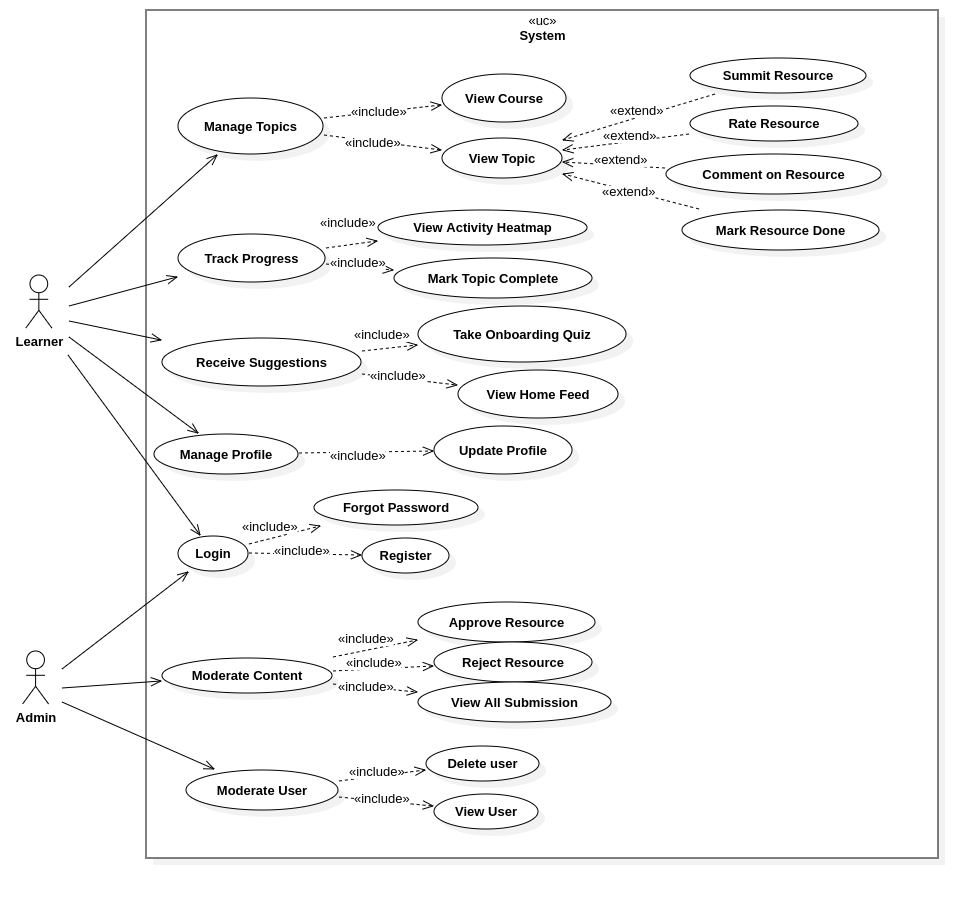
\includegraphics[width=0.95\textwidth]{ucd.png}}{\missingfig{ucd.png}{Overall Use Case Diagram}}
\caption{Overall Use Case Diagram}
\label{fig:ucd-overall}
\end{figure}

\subsection{Use Case Diagram -- Authentication}

Figure~\ref{fig:ucd-auth} zooms into the authentication module, covering registration, login, and password reset. These three use cases form the security boundary for all other interactions.

\begin{figure}[H]
\centering
\IfFileExists{ucd_auth.png}{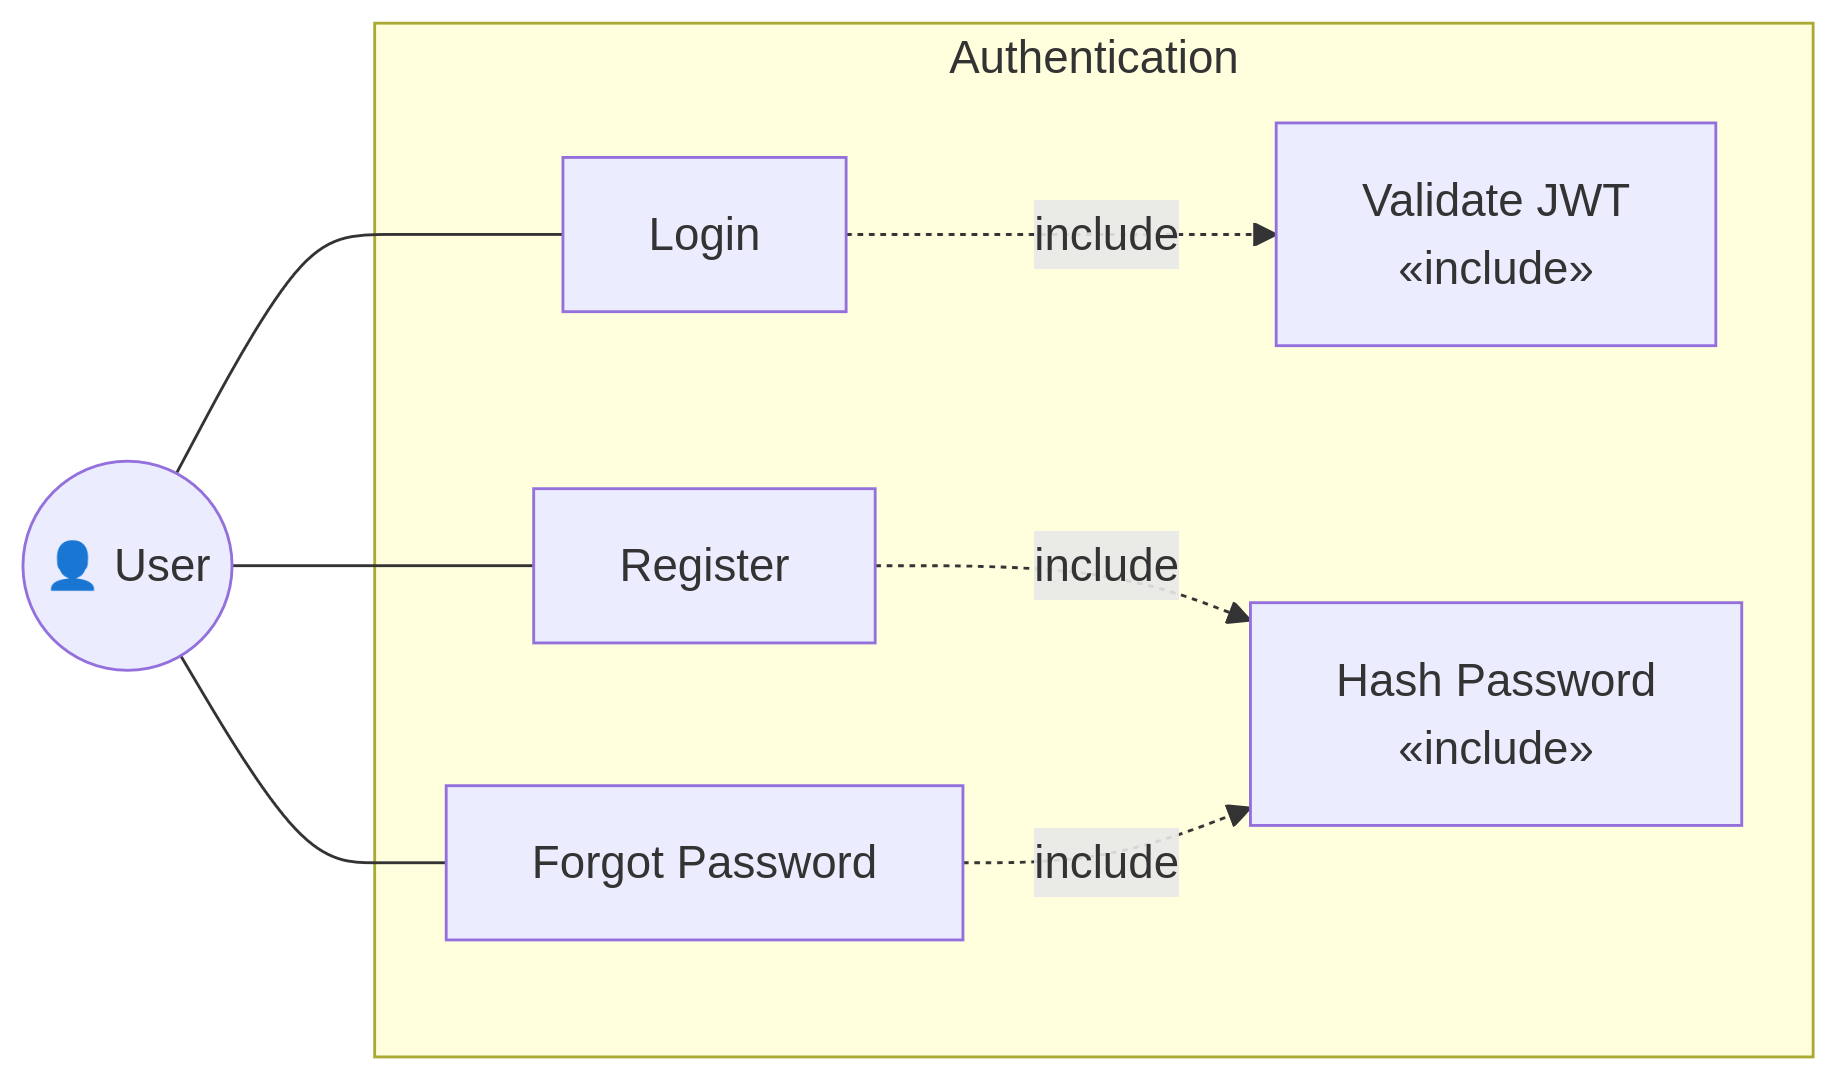
\includegraphics[width=0.75\textwidth]{ucd_auth.png}}{\missingfig{ucd\_auth.png}{Authentication Use Case Diagram}}
\caption{Use Case Diagram -- Authentication Module}
\label{fig:ucd-auth}
\end{figure}

\subsection{Use Case Diagram -- Resource Management}

Figure~\ref{fig:ucd-resource} shows the resource management flow, from learner submission through admin review to public availability. The separation between the submission (Learner) and approval (Admin) actors is the central design principle of the content pipeline.

\begin{figure}[H]
\centering
\IfFileExists{ucd_resource.png}{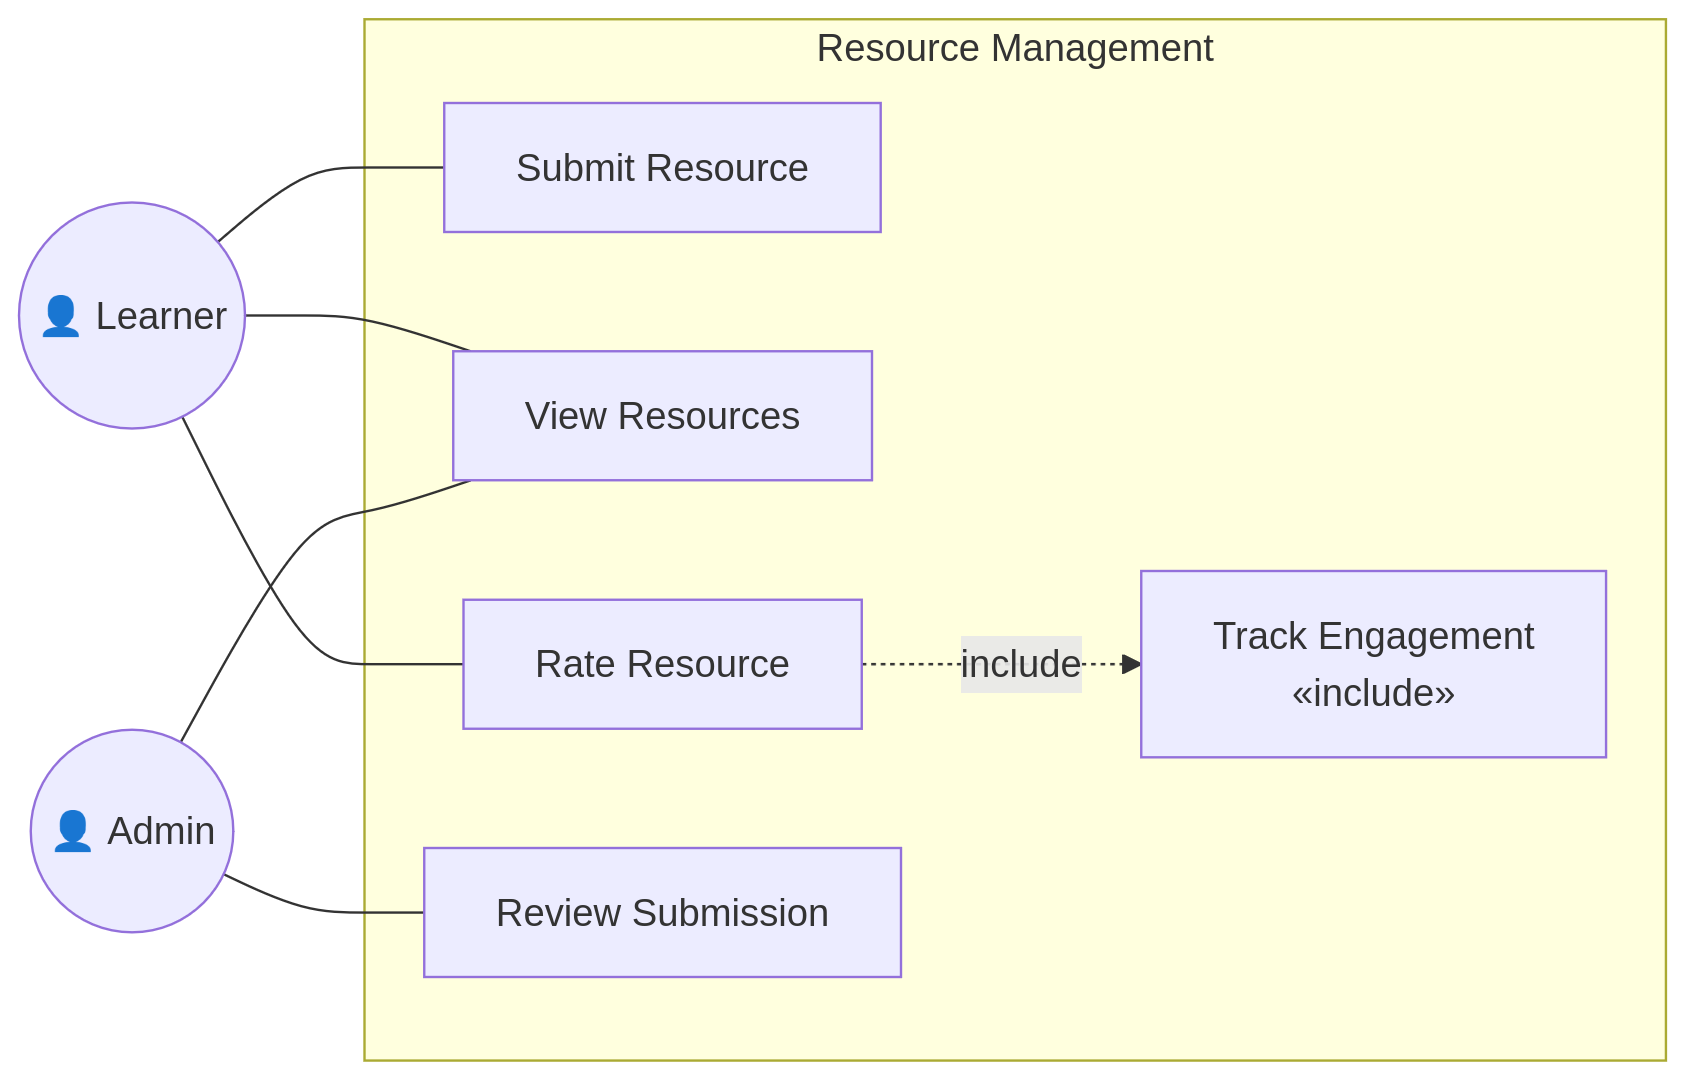
\includegraphics[width=0.75\textwidth]{ucd_resource.png}}{\missingfig{ucd\_resource.png}{Resource Management Use Case Diagram}}
\caption{Use Case Diagram -- Resource Management}
\label{fig:ucd-resource}
\end{figure}

\subsection{Detailed Use Cases}

The following tables provide detailed specifications for the three most complex use cases. The remaining use cases (UC-01 through UC-03, UC-05, UC-06, UC-09, UC-10) follow standard CRUD patterns and are fully covered by the sequence diagrams in Chapter 6.

\begin{longtable}{p{0.2\textwidth} p{0.72\textwidth}}
\caption{UC-04: Rate a Resource}\label{tab:uc04}\\
\toprule
\textbf{Field} & \textbf{Detail} \\
\midrule
\endfirsthead
\toprule
\textbf{Field} & \textbf{Detail} \\
\midrule
\endhead
Use Case ID & UC-04 \\
Name & Rate a Resource \\
Actor & Learner \\
Precondition & User is logged in and has accessed a topic detail page. \\
Main Flow & 1. User views a resource on a topic page. \newline 2. User selects a star rating (1--5). \newline 3. Optionally provides a reason if rating is low (1--2 stars). \newline 4. System saves the rating and updates the recommendation model. \\
Postcondition & Rating is stored. Future recommendations reflect this preference. \\
Exception & If stars not in range 1--5, system returns HTTP 400. \\
\bottomrule
\end{longtable}

\begin{longtable}{p{0.2\textwidth} p{0.72\textwidth}}
\caption{UC-07: View Personalised Recommendations}\label{tab:uc07}\\
\toprule
\textbf{Field} & \textbf{Detail} \\
\midrule
\endfirsthead
\toprule
\textbf{Field} & \textbf{Detail} \\
\midrule
\endhead
Use Case ID & UC-07 \\
Name & View Personalised Recommendations \\
Actor & Learner \\
Precondition & User is logged in. \\
Main Flow & 1. User opens a topic detail page or the home feed. \newline 2. System computes similarity between the user and all others. \newline 3. Resources rated highly by similar users are ranked and returned. \newline 4. User sees up to 6 recommended resources from other topics. \\
Postcondition & Recommendations are displayed. \\
Exception & If user has no ratings, system falls back to popularity ranking boosted by onboarding answers. \\
\bottomrule
\end{longtable}

\begin{longtable}{p{0.2\textwidth} p{0.72\textwidth}}
\caption{UC-08: Admin Review Submission}\label{tab:uc08}\\
\toprule
\textbf{Field} & \textbf{Detail} \\
\midrule
\endfirsthead
\toprule
\textbf{Field} & \textbf{Detail} \\
\midrule
\endhead
Use Case ID & UC-08 \\
Name & Review Pending Resource \\
Actor & Admin \\
Precondition & At least one resource is in \texttt{pending} status. \\
Main Flow & 1. Admin opens the Admin Review page. \newline 2. System lists all pending submissions with title, URL, submitter, and topic. \newline 3. Admin clicks Approve or Reject. \newline 4. Resource status is updated to \texttt{approved} or \texttt{rejected}. \\
Postcondition & Approved resources become visible to all learners. Rejected resources are hidden. \\
\bottomrule
\end{longtable}

Together, these use cases define the interaction boundaries of the system. The next chapter describes the development methodology and testing strategy used to implement them.

% ============================================================
% CHAPTER 3 -- METHODOLOGY
% ============================================================
\chapter{Methodology}

This chapter covers how the project was developed, how the code was managed, and how it was tested.

\section{Development Approach}

Development ran from early April to late June 2026, roughly three months. Instead of designing everything upfront and building it all at the end, the work was split into feature phases \cite{beck2001}. Each phase had a clear goal -- get one group of features working end-to-end -- before moving to the next. This meant bugs and integration problems showed up early when they were still easy to fix, rather than piling up at the end.

Table~\ref{tab:timeline} shows what was done each phase.

\begin{longtable}{p{0.25\textwidth} p{0.65\textwidth}}
\caption{Development Timeline}\label{tab:timeline}\\
\toprule
\textbf{Period} & \textbf{Work Done} \\
\midrule
April (Weeks 1--2) & Project setup, database schema, auth (register, login, JWT) \\
April (Weeks 3--4) & Topics, courses, prerequisite links, seed data \\
May (Weeks 1--2) & Resource upload, admin review, ratings \\
May (Weeks 3--4) & Engagement tracking, recommendation engine \\
June (Weeks 1--2) & Onboarding quiz, cold-start, progress tracking, home feed \\
June (Weeks 3--4) & UI, bug fixes, deployment, report \\
\bottomrule
\end{longtable}

The schema also evolved during development. The \texttt{version} column on resources, for example, was added in May when it became clear that tracking resource updates might be useful later.

\section{Version Control}

Git was used throughout, with commits organised by feature. The repository is on GitHub. Both Render (backend) and Vercel (frontend) are configured to auto-deploy on every push to \texttt{main}, so the live site always reflects the latest version. A GitHub Actions workflow also runs the test suite on every push.

\section{Testing Strategy}

Testing was done at two levels:

\begin{enumerate}
  \item \textbf{Automated tests} using \texttt{pytest} and the FastAPI test client. These cover the auth flows and the recommender algorithm (scoring formula and cold-start fallback).
  \item \textbf{Manual end-to-end testing} on the deployed site, done by several classmates across different devices and browsers. This caught two bugs -- a CORS ordering issue and a missing route -- that are documented in Chapter 9.
\end{enumerate}

% ============================================================
% CHAPTER 4 -- SYSTEM ARCHITECTURE
% ============================================================
\chapter{System Architecture}

This chapter describes how the system is structured, how the layers communicate, and where everything is deployed.

\section{High-Level Architecture}

Opic is a standard client-server application. The frontend is a React SPA, the backend is a FastAPI REST API, and the database is PostgreSQL. Figure~\ref{fig:arch} shows how they connect.

\begin{figure}[H]
\centering
\IfFileExists{arch.png}{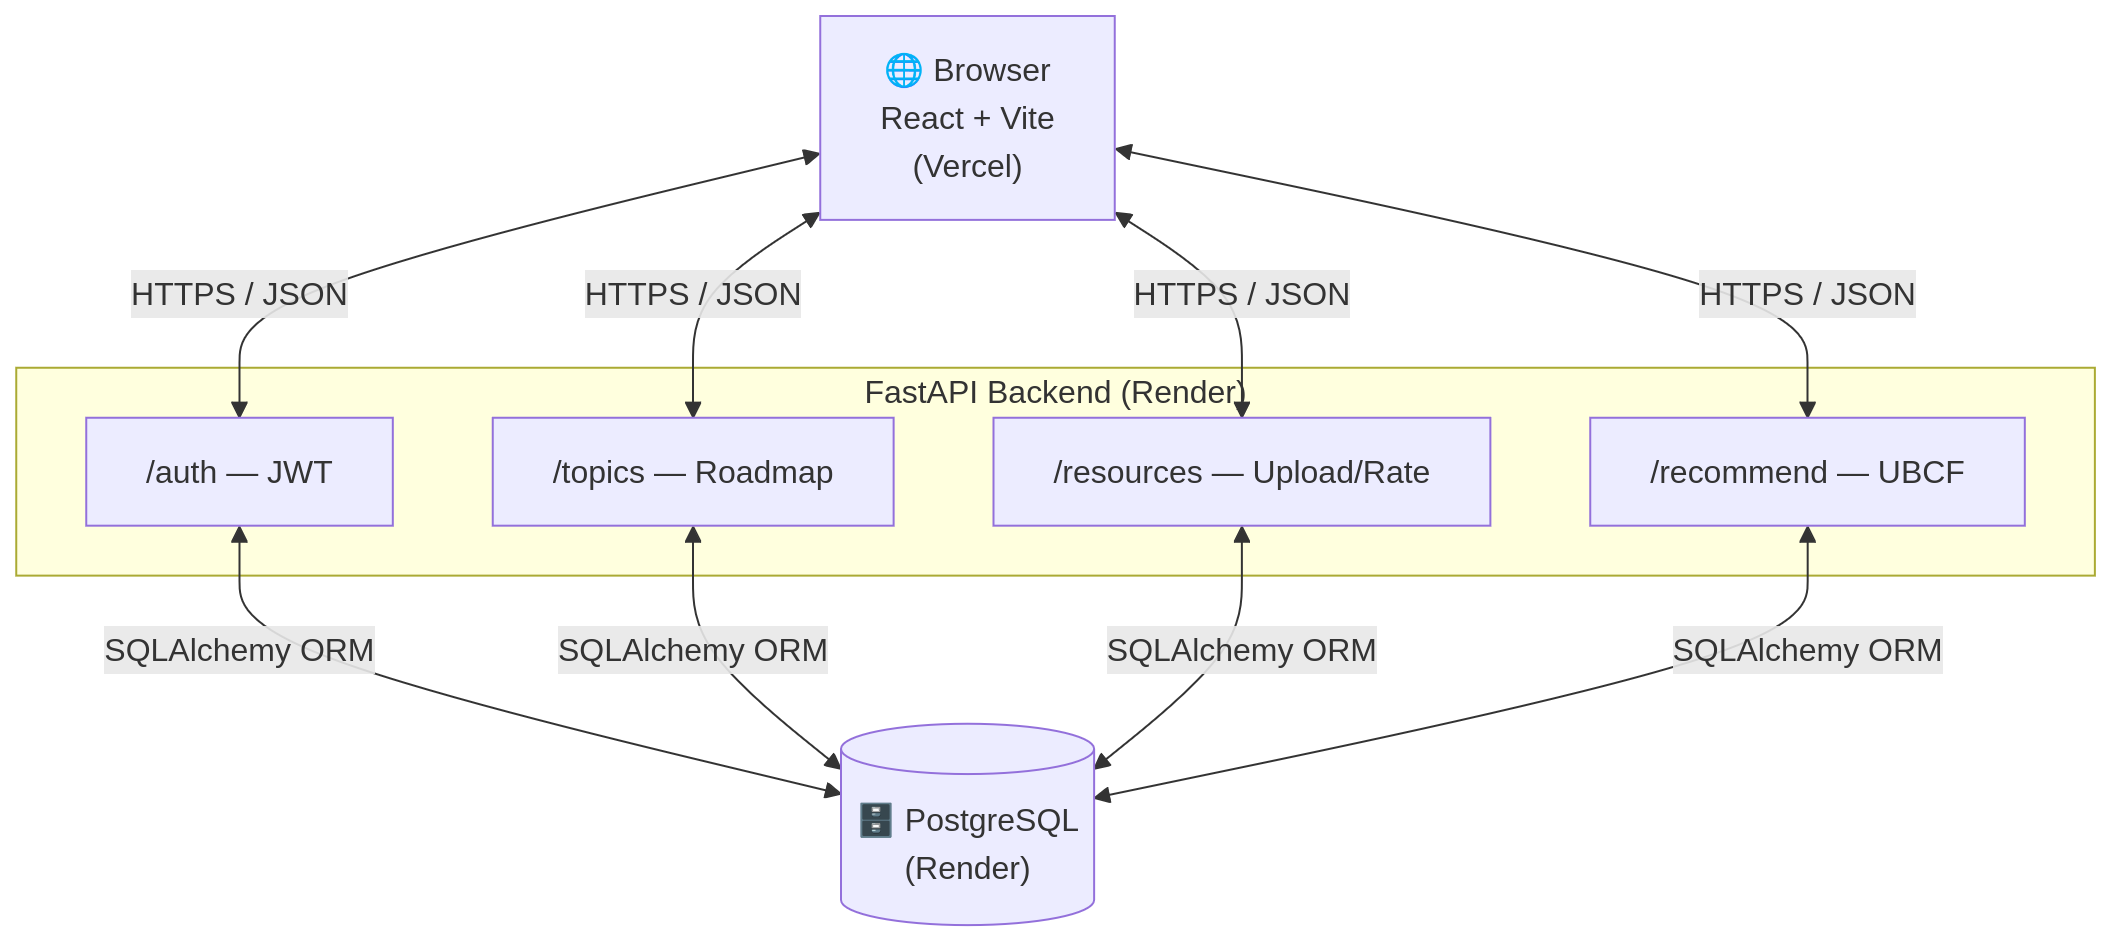
\includegraphics[width=0.85\textwidth]{arch.png}}{\missingfig{arch.png}{System Architecture Diagram}}
\caption{System Architecture Diagram}
\label{fig:arch}
\end{figure}

All communication is over HTTPS with JSON. There is no WebSocket -- everything is request/response. This keeps the system simple and easy to test.

\section{Frontend}

The frontend is built with React 18 and Vite. \texttt{axios} handles all API calls, with an interceptor that attaches the JWT token to every request. React Router v6 handles navigation. Auth state (user object and token) is stored in a React Context, initialised from \texttt{localStorage} on page load so sessions survive refreshes.

\section{Backend}

The backend uses FastAPI. It is split into four layers:

\begin{itemize}
  \item \texttt{app/api/} -- route handlers (\texttt{auth}, \texttt{topics}, \texttt{resources}, \texttt{recommend})
  \item \texttt{app/models/} -- SQLAlchemy ORM models
  \item \texttt{app/services/} -- business logic (recommender)
  \item \texttt{app/core/} -- database setup, JWT, password hashing
\end{itemize}

FastAPI generates interactive API docs automatically at \texttt{/docs}, which was useful during development.

\section{Deployment}

Everything runs on free-tier cloud services. Table~\ref{tab:deploy} summarises the setup.

\begin{longtable}{p{0.2\textwidth} p{0.3\textwidth} p{0.4\textwidth}}
\caption{Deployment Infrastructure}\label{tab:deploy}\\
\toprule
\textbf{Component} & \textbf{Service} & \textbf{Notes} \\
\midrule
Frontend & Vercel & Static bundle, global CDN, auto-deploy on push \\
Backend & Render & Python web service, persistent process \\
Database & Render PostgreSQL & Managed PostgreSQL, automatic backups \\
\bottomrule
\end{longtable}

Both Vercel and Render are configured to redeploy automatically on every push to \texttt{main}. GitHub Actions runs the test suite first, so a failing test blocks the deploy.

% ============================================================
% CHAPTER 5 -- DATABASE DESIGN
% ============================================================
\chapter{Database Design}

This chapter presents the database schema that stores all application data. The schema was designed to support the functional requirements from Chapter 2 while keeping query complexity manageable and enforcing data integrity through database-level constraints. The design consists of nine tables centred on three core entities: \texttt{users}, \texttt{topics}, and \texttt{resources}.

\section{Entity-Relationship Overview}

Figure~\ref{fig:erd} shows the entity-relationship diagram for the complete schema. The diagram illustrates how the nine tables relate to one another through foreign keys and composite primary keys.

\begin{figure}[H]
\centering
\IfFileExists{erd.png}{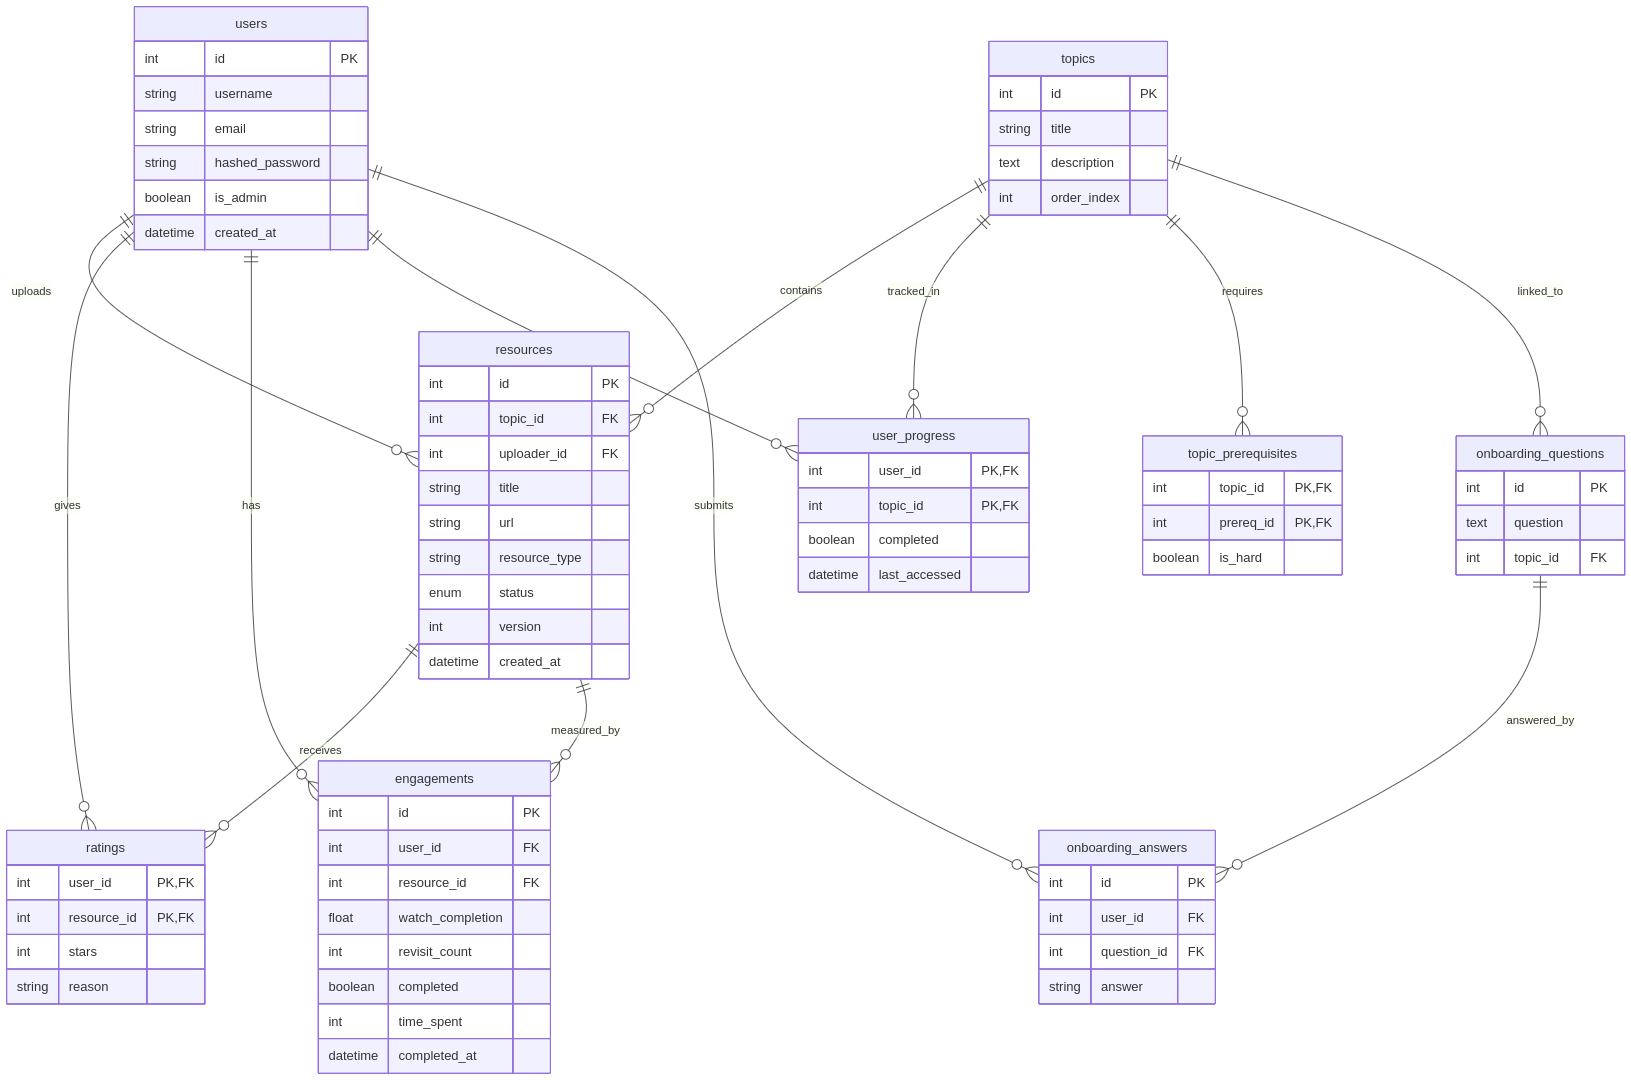
\includegraphics[width=0.9\textwidth]{erd.png}}{\missingfig{erd.png}{Entity-Relationship Diagram showing the nine tables and their relationships}}
\caption{Entity-Relationship Diagram}
\label{fig:erd}
\end{figure}

The three central tables (\texttt{users}, \texttt{topics}, \texttt{resources}) are surrounded by supporting tables that capture interactions between them. The \texttt{ratings} and \texttt{engagements} tables record user-resource interactions. The \texttt{user\_progress} table records user-topic interactions. The \texttt{topic\_prerequisites} table captures topic-topic relationships. The \texttt{onboarding\_questions} and \texttt{onboarding\_answers} tables support the cold-start recommendation flow.

\section{Table Descriptions}

The following subsections describe each table in detail. For each table, the column definitions are followed by a brief explanation of its role in the system.

\subsection{users}

The \texttt{users} table is the foundation of the authentication system. Every action in the platform is associated with a user record, either as the actor (ratings, submissions) or as the target (admin management).

\begin{longtable}{p{0.22\textwidth} p{0.18\textwidth} p{0.5\textwidth}}
\caption{Table: users}\label{tab:users}\\
\toprule
\textbf{Column} & \textbf{Type} & \textbf{Description} \\
\midrule
\endfirsthead
\toprule
\textbf{Column} & \textbf{Type} & \textbf{Description} \\
\midrule
\endhead
id & INTEGER (PK) & Auto-incremented primary key \\
username & VARCHAR & Unique display name \\
email & VARCHAR & Unique email address used for login \\
hashed\_password & VARCHAR & bcrypt-hashed password, never stored in plain text \\
is\_admin & BOOLEAN & If true, user has admin privileges \\
created\_at & DATETIME & Account creation timestamp \\
\bottomrule
\end{longtable}

The \texttt{is\_admin} boolean is a simple but effective role flag. Its main limitation -- the absence of intermediate roles -- is acknowledged in Chapter 9.

\subsection{topics}

The \texttt{topics} table defines the learning map. Each topic belongs to a logical course grouping encoded in the title field.

\begin{longtable}{p{0.22\textwidth} p{0.18\textwidth} p{0.5\textwidth}}
\caption{Table: topics}\label{tab:topics}\\
\toprule
\textbf{Column} & \textbf{Type} & \textbf{Description} \\
\midrule
\endfirsthead
\toprule
\textbf{Column} & \textbf{Type} & \textbf{Description} \\
\midrule
\endhead
id & INTEGER (PK) & Auto-incremented primary key \\
title & VARCHAR & Topic title (format: ``Course: Topic'') \\
description & TEXT & Short explanation of what the topic covers \\
order\_index & INTEGER & Display order within a course \\
\bottomrule
\end{longtable}

\subsection{topic\_prerequisites}

This junction table encodes directed prerequisite relationships between topics. The \texttt{is\_hard} flag distinguishes mandatory prerequisites from suggested ones, enabling future UI differentiation.

\begin{longtable}{p{0.22\textwidth} p{0.18\textwidth} p{0.5\textwidth}}
\caption{Table: topic\_prerequisites}\label{tab:prereqs}\\
\toprule
\textbf{Column} & \textbf{Type} & \textbf{Description} \\
\midrule
\endfirsthead
\toprule
\textbf{Column} & \textbf{Type} & \textbf{Description} \\
\midrule
\endhead
topic\_id & INTEGER (PK, FK) & The topic that has the requirement \\
prereq\_id & INTEGER (PK, FK) & The topic that must be completed first \\
is\_hard & BOOLEAN & True = mandatory prerequisite; False = suggested only \\
\bottomrule
\end{longtable}

\subsection{resources}

The \texttt{resources} table is at the centre of the content pipeline. The \texttt{status} column gates which resources are visible to learners; only \texttt{approved} resources are returned by the topic detail endpoint.

\begin{longtable}{p{0.22\textwidth} p{0.18\textwidth} p{0.5\textwidth}}
\caption{Table: resources}\label{tab:resources}\\
\toprule
\textbf{Column} & \textbf{Type} & \textbf{Description} \\
\midrule
\endfirsthead
\toprule
\textbf{Column} & \textbf{Type} & \textbf{Description} \\
\midrule
\endhead
id & INTEGER (PK) & Auto-incremented primary key \\
topic\_id & INTEGER (FK) & The topic this resource belongs to \\
uploader\_id & INTEGER (FK) & The user who submitted this resource \\
title & VARCHAR & Resource title (max 200 characters) \\
url & VARCHAR & Full URL (must be http or https) \\
resource\_type & VARCHAR & Either \texttt{video} or \texttt{article} \\
status & ENUM & One of: \texttt{pending}, \texttt{approved}, \texttt{rejected} \\
version & INTEGER & Reserved for future update support \\
created\_at & DATETIME & Submission timestamp \\
\bottomrule
\end{longtable}

\subsection{ratings}

The \texttt{ratings} table records each user's explicit feedback on a resource. It feeds directly into the recommendation engine's user-resource matrix.

\begin{longtable}{p{0.22\textwidth} p{0.18\textwidth} p{0.5\textwidth}}
\caption{Table: ratings}\label{tab:ratings}\\
\toprule
\textbf{Column} & \textbf{Type} & \textbf{Description} \\
\midrule
\endfirsthead
\toprule
\textbf{Column} & \textbf{Type} & \textbf{Description} \\
\midrule
\endhead
user\_id & INTEGER (PK, FK) & The user who gave the rating \\
resource\_id & INTEGER (PK, FK) & The resource being rated \\
stars & INTEGER & Rating value from 1 to 5 \\
reason & VARCHAR & Optional feedback text for low ratings (1--2 stars) \\
\bottomrule
\end{longtable}

The composite primary key \texttt{(user\_id, resource\_id)} enforces one rating per user per resource. Submitting a new rating for the same resource updates the existing row rather than creating a duplicate.

\subsection{engagements}

The \texttt{engagements} table captures implicit feedback signals that supplement the explicit star ratings. These signals are combined with the star rating to produce the weighted engagement score used in the recommendation engine (see Chapter 6).

\begin{longtable}{p{0.22\textwidth} p{0.18\textwidth} p{0.5\textwidth}}
\caption{Table: engagements}\label{tab:engagements}\\
\toprule
\textbf{Column} & \textbf{Type} & \textbf{Description} \\
\midrule
\endfirsthead
\toprule
\textbf{Column} & \textbf{Type} & \textbf{Description} \\
\midrule
\endhead
id & INTEGER (PK) & Auto-incremented primary key \\
user\_id & INTEGER (FK) & The user whose engagement is tracked \\
resource\_id & INTEGER (FK) & The resource being engaged with \\
watch\_completion & FLOAT & Ratio 0.0--1.0 of how much was watched/read \\
revisit\_count & INTEGER & Number of times the user returned to this resource \\
completed & BOOLEAN & Whether the user marked this resource as done \\
time\_spent & INTEGER & Total seconds spent on the resource \\
completed\_at & DATETIME & Timestamp when the user first marked it complete \\
\bottomrule
\end{longtable}

\subsection{user\_progress}

The \texttt{user\_progress} table tracks topic-level completion, which is distinct from resource-level engagement. A user can mark a topic as complete even if they have not interacted with every resource under it.

\begin{longtable}{p{0.22\textwidth} p{0.18\textwidth} p{0.5\textwidth}}
\caption{Table: user\_progress}\label{tab:progress}\\
\toprule
\textbf{Column} & \textbf{Type} & \textbf{Description} \\
\midrule
\endfirsthead
\toprule
\textbf{Column} & \textbf{Type} & \textbf{Description} \\
\midrule
\endhead
user\_id & INTEGER (PK, FK) & The user tracking progress \\
topic\_id & INTEGER (PK, FK) & The topic being tracked \\
completed & BOOLEAN & Whether the topic is marked as completed \\
last\_accessed & DATETIME & Last time the user visited this topic \\
\bottomrule
\end{longtable}

\subsection{onboarding\_questions and onboarding\_answers}

These two tables together support the cold-start recommendation fallback. Each question is linked to a topic; a positive answer boosts that topic's resources during the initial recommendation pass for a new user with no ratings.

\begin{longtable}{p{0.22\textwidth} p{0.18\textwidth} p{0.5\textwidth}}
\caption{Table: onboarding\_questions}\label{tab:oq}\\
\toprule
\textbf{Column} & \textbf{Type} & \textbf{Description} \\
\midrule
\endfirsthead
\toprule
\textbf{Column} & \textbf{Type} & \textbf{Description} \\
\midrule
\endhead
id & INTEGER (PK) & Auto-incremented primary key \\
question & TEXT & The question text shown to the user \\
topic\_id & INTEGER (FK) & Maps this question to a topic for cold-start boosting \\
\bottomrule
\end{longtable}

\begin{longtable}{p{0.22\textwidth} p{0.18\textwidth} p{0.5\textwidth}}
\caption{Table: onboarding\_answers}\label{tab:oa}\\
\toprule
\textbf{Column} & \textbf{Type} & \textbf{Description} \\
\midrule
\endfirsthead
\toprule
\textbf{Column} & \textbf{Type} & \textbf{Description} \\
\midrule
\endhead
id & INTEGER (PK) & Auto-incremented primary key \\
user\_id & INTEGER (FK) & The user who answered \\
question\_id & INTEGER (FK) & The question being answered \\
answer & VARCHAR & Free-text answer; answers containing negative words (no, never, don't) are excluded from boosting \\
\bottomrule
\end{longtable}

\section{Key Design Decisions}

Several non-obvious choices were made during schema design. The rationale for the most important ones is summarised below:

\begin{itemize}
  \item \textbf{Composite primary keys} on \texttt{ratings} and \texttt{user\_progress} prevent duplicate rows naturally without requiring application-level uniqueness checks.
  \item \textbf{Indexed columns:} \texttt{(topic\_id, status)} on resources and \texttt{(user\_id, completed)} on engagements speed up the most frequent queries (fetching approved resources for a topic, and building the recommendation matrix).
  \item \textbf{Soft/hard prerequisites:} The \texttt{is\_hard} boolean distinguishes mandatory prerequisites from suggested ones, allowing the UI to differentiate them in a future iteration.
  \item \textbf{Resource versioning:} The \texttt{version} column was included for future support of resource updates without losing rating history. It is not yet used by the current implementation.
  \item \textbf{Rating computed at query time:} Rather than storing a pre-computed average, the overall rating is calculated from the \texttt{ratings} table on each request. This ensures the displayed value is always accurate immediately after any new rating is submitted, without requiring a background synchronisation job.
\end{itemize}

With the schema defined, the next chapter walks through how each use case is implemented on top of it.

% ============================================================
% CHAPTER 6 -- USE CASE IMPLEMENTATION
% ============================================================
\chapter{Use Case Implementation}

This chapter describes how each use case identified in Chapter 2 was implemented. For each group of related use cases, a sequence diagram illustrates the interaction flow between the browser, the React frontend, the FastAPI backend, and the database. Code excerpts are included where the implementation is non-trivial or academically significant.

\section{Use Case Implementation Overview}

Before examining each use case individually, Table~\ref{tab:uc-impl-summary} provides a consolidated view of all use cases, the main endpoint they invoke, and the section in this chapter where they are detailed.

\begin{longtable}{p{0.12\textwidth} p{0.28\textwidth} p{0.30\textwidth} p{0.18\textwidth}}
\caption{Use Case Implementation Summary}\label{tab:uc-impl-summary}\\
\toprule
\textbf{ID} & \textbf{Name} & \textbf{Main Endpoint} & \textbf{Section} \\
\midrule
\endfirsthead
\toprule
\textbf{ID} & \textbf{Name} & \textbf{Main Endpoint} & \textbf{Section} \\
\midrule
\endhead
UC-01 & Register Account & \texttt{POST /auth/register} & \ref{sec:impl-auth} \\
UC-02 & Log In & \texttt{POST /auth/login} & \ref{sec:impl-auth} \\
UC-03 & Reset Password & \texttt{POST /auth/reset-password} & \ref{sec:impl-auth} \\
UC-04 & Rate a Resource & \texttt{POST /resources/\{id\}/rate} & \ref{sec:impl-resources} \\
UC-05 & Submit a Resource & \texttt{POST /resources/} & \ref{sec:impl-resources} \\
UC-06 & Track Topic Progress & \texttt{POST /topics/\{id\}/progress} & \ref{sec:impl-progress} \\
UC-07 & View Recommendations & \texttt{GET /recommend/\{user\_id\}} & \ref{sec:impl-rec} \\
UC-08 & Admin Review Submission & \texttt{POST /resources/\{id\}/review} & \ref{sec:impl-adminreview} \\
UC-09 & Manage Users & \texttt{GET /auth/users}, \texttt{DELETE /auth/users/\{id\}} & \ref{sec:impl-adminreview} \\
UC-10 & Complete Onboarding Quiz & \texttt{POST /auth/onboarding} & \ref{sec:impl-auth} \\
\bottomrule
\end{longtable}

The sections that follow examine each group in turn, starting with authentication.

\section{Authentication}
\label{sec:impl-auth}

Authentication covers three use cases: registration (UC-01), login (UC-02), and password reset (UC-03), as well as the onboarding quiz (UC-10) that runs immediately after registration. Together these use cases define the security boundary for the entire system.

\subsection{Register Sequence}

Figure~\ref{fig:seq-register} shows the sequence when a new user creates an account. The backend hashes the password with bcrypt before writing to the database -- the plain-text password never touches persistent storage.

\begin{figure}[H]
\centering
\IfFileExists{seq_register.png}{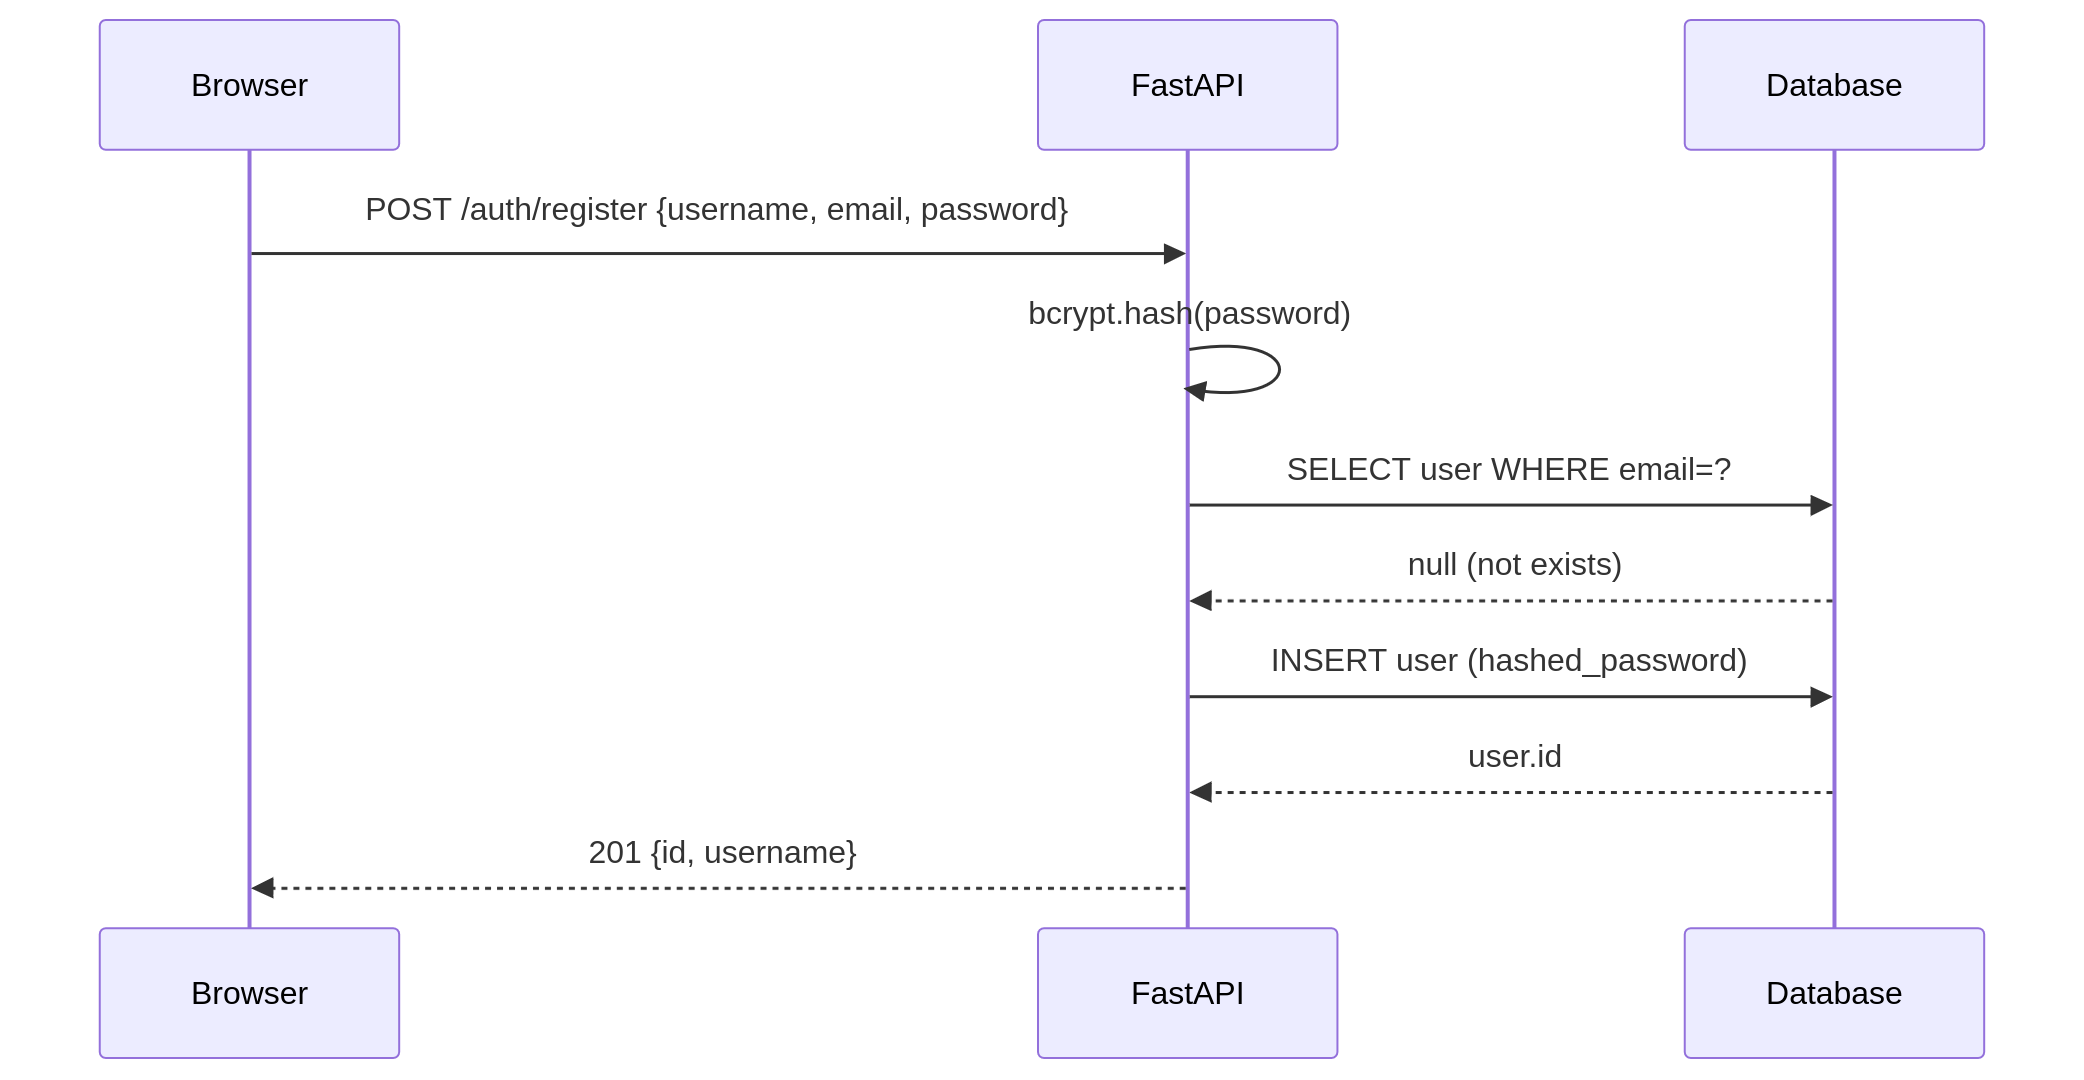
\includegraphics[width=0.75\textwidth]{seq_register.png}}{\missingfig{seq\_register.png}{Sequence Diagram -- User Registration: Browser → React → POST /auth/register → bcrypt hash → DB insert → return 201}}
\caption{Sequence Diagram -- User Registration}
\label{fig:seq-register}
\end{figure}

\subsection{Login Sequence}

Figure~\ref{fig:seq-login} shows the events when a user logs in. On success, the server generates a signed JWT containing the user's ID and \texttt{is\_admin} flag. The token is stored in \texttt{localStorage} by the frontend and attached to every subsequent request in the \texttt{Authorization: Bearer} header.

\begin{figure}[H]
\centering
\IfFileExists{seq_login.png}{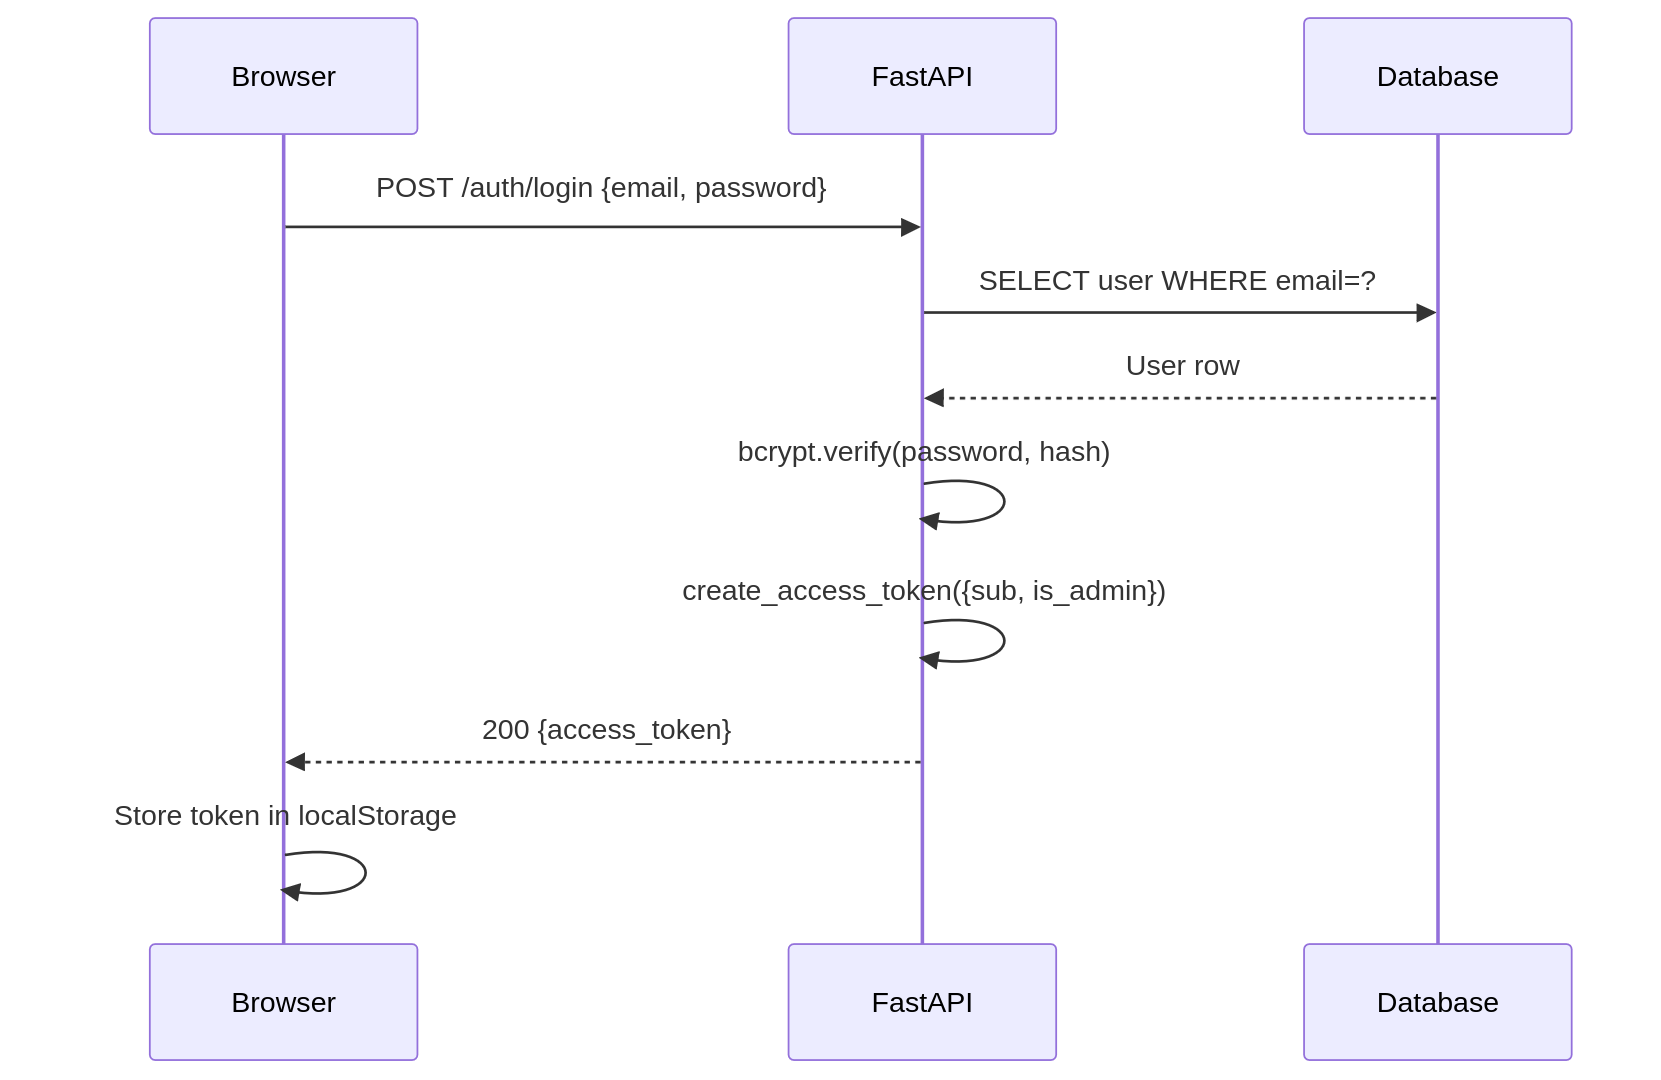
\includegraphics[width=0.75\textwidth]{seq_login.png}}{\missingfig{seq\_login.png}{Sequence Diagram -- User Login: Browser → React → POST /auth/login → bcrypt verify → JWT sign → return token}}
\caption{Sequence Diagram -- User Login}
\label{fig:seq-login}
\end{figure}

Passwords are verified using the \texttt{passlib} library \cite{passlib} with the bcrypt scheme \cite{provos1999}. A separate password reset flow (UC-03) sends a 6-character alphanumeric code with a 10-minute expiry to the user's registered email address via SMTP using the \texttt{aiosmtplib} library \cite{aiosmtplib}.

\section{Resource Management}
\label{sec:impl-resources}

Resource management covers the submission (UC-05), rating (UC-04), and admin review (UC-08) use cases. These three flows together define the full content lifecycle on the platform.

\subsection{Resource Submission Sequence}

Figure~\ref{fig:seq-submit} shows how a learner submits a resource for review. The resource is created with \texttt{status = pending} and is not visible to other learners until an admin approves it.

\begin{figure}[H]
\centering
\IfFileExists{seq_submit.png}{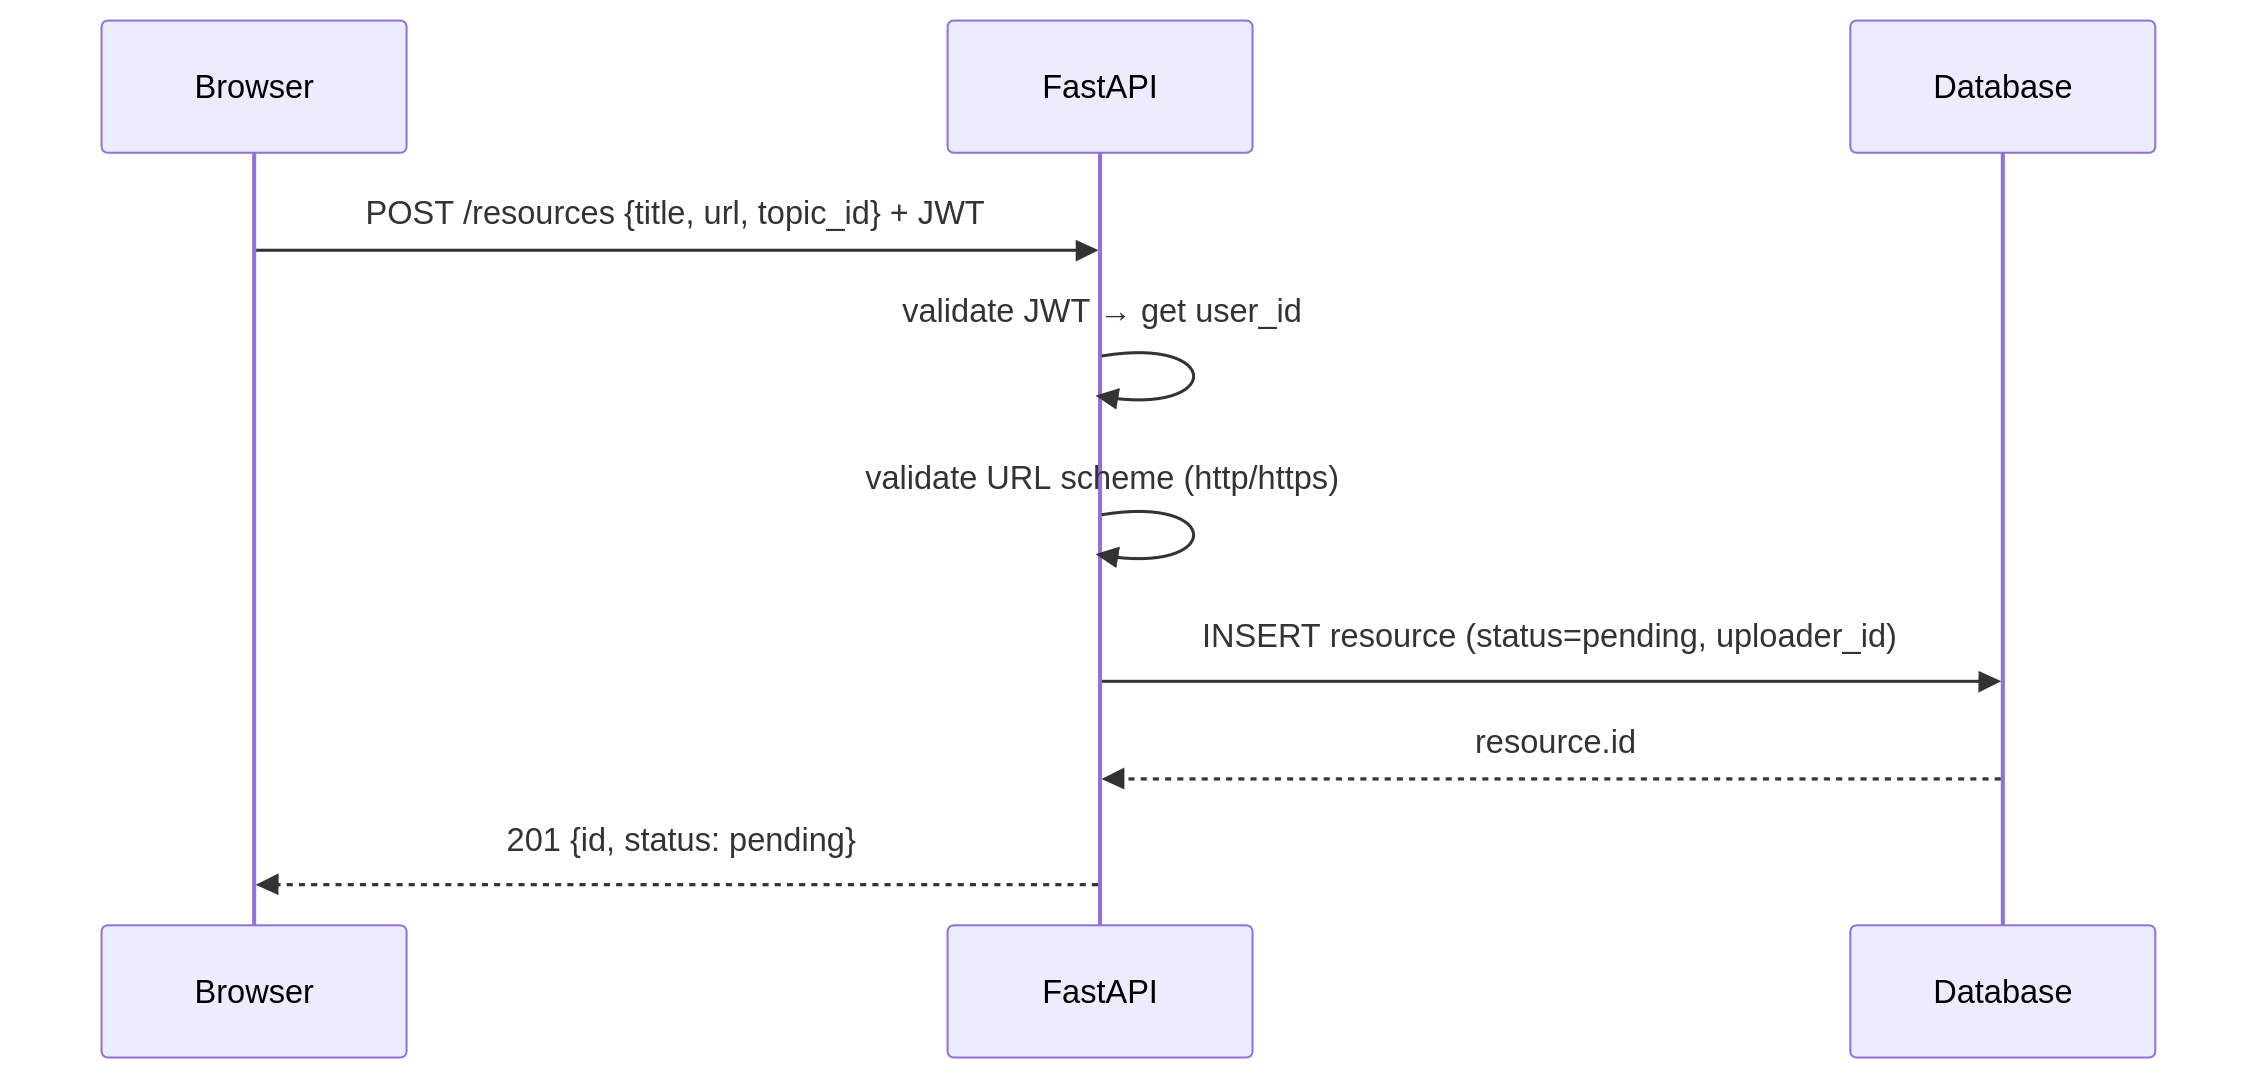
\includegraphics[width=0.75\textwidth]{seq_submit.png}}{\missingfig{seq\_submit.png}{Sequence Diagram -- Resource Submission: learner POSTs resource → saved as pending → not visible until approved}}
\caption{Sequence Diagram -- Resource Submission}
\label{fig:seq-submit}
\end{figure}

\subsection{Admin Review Sequence}

Figure~\ref{fig:seq-review} shows the flow from submission to admin approval. When the admin calls the review endpoint with \texttt{approved=true}, the resource status is updated to \texttt{approved} and becomes visible on the topic detail page for all learners.

\begin{figure}[H]
\centering
\IfFileExists{seq_review.png}{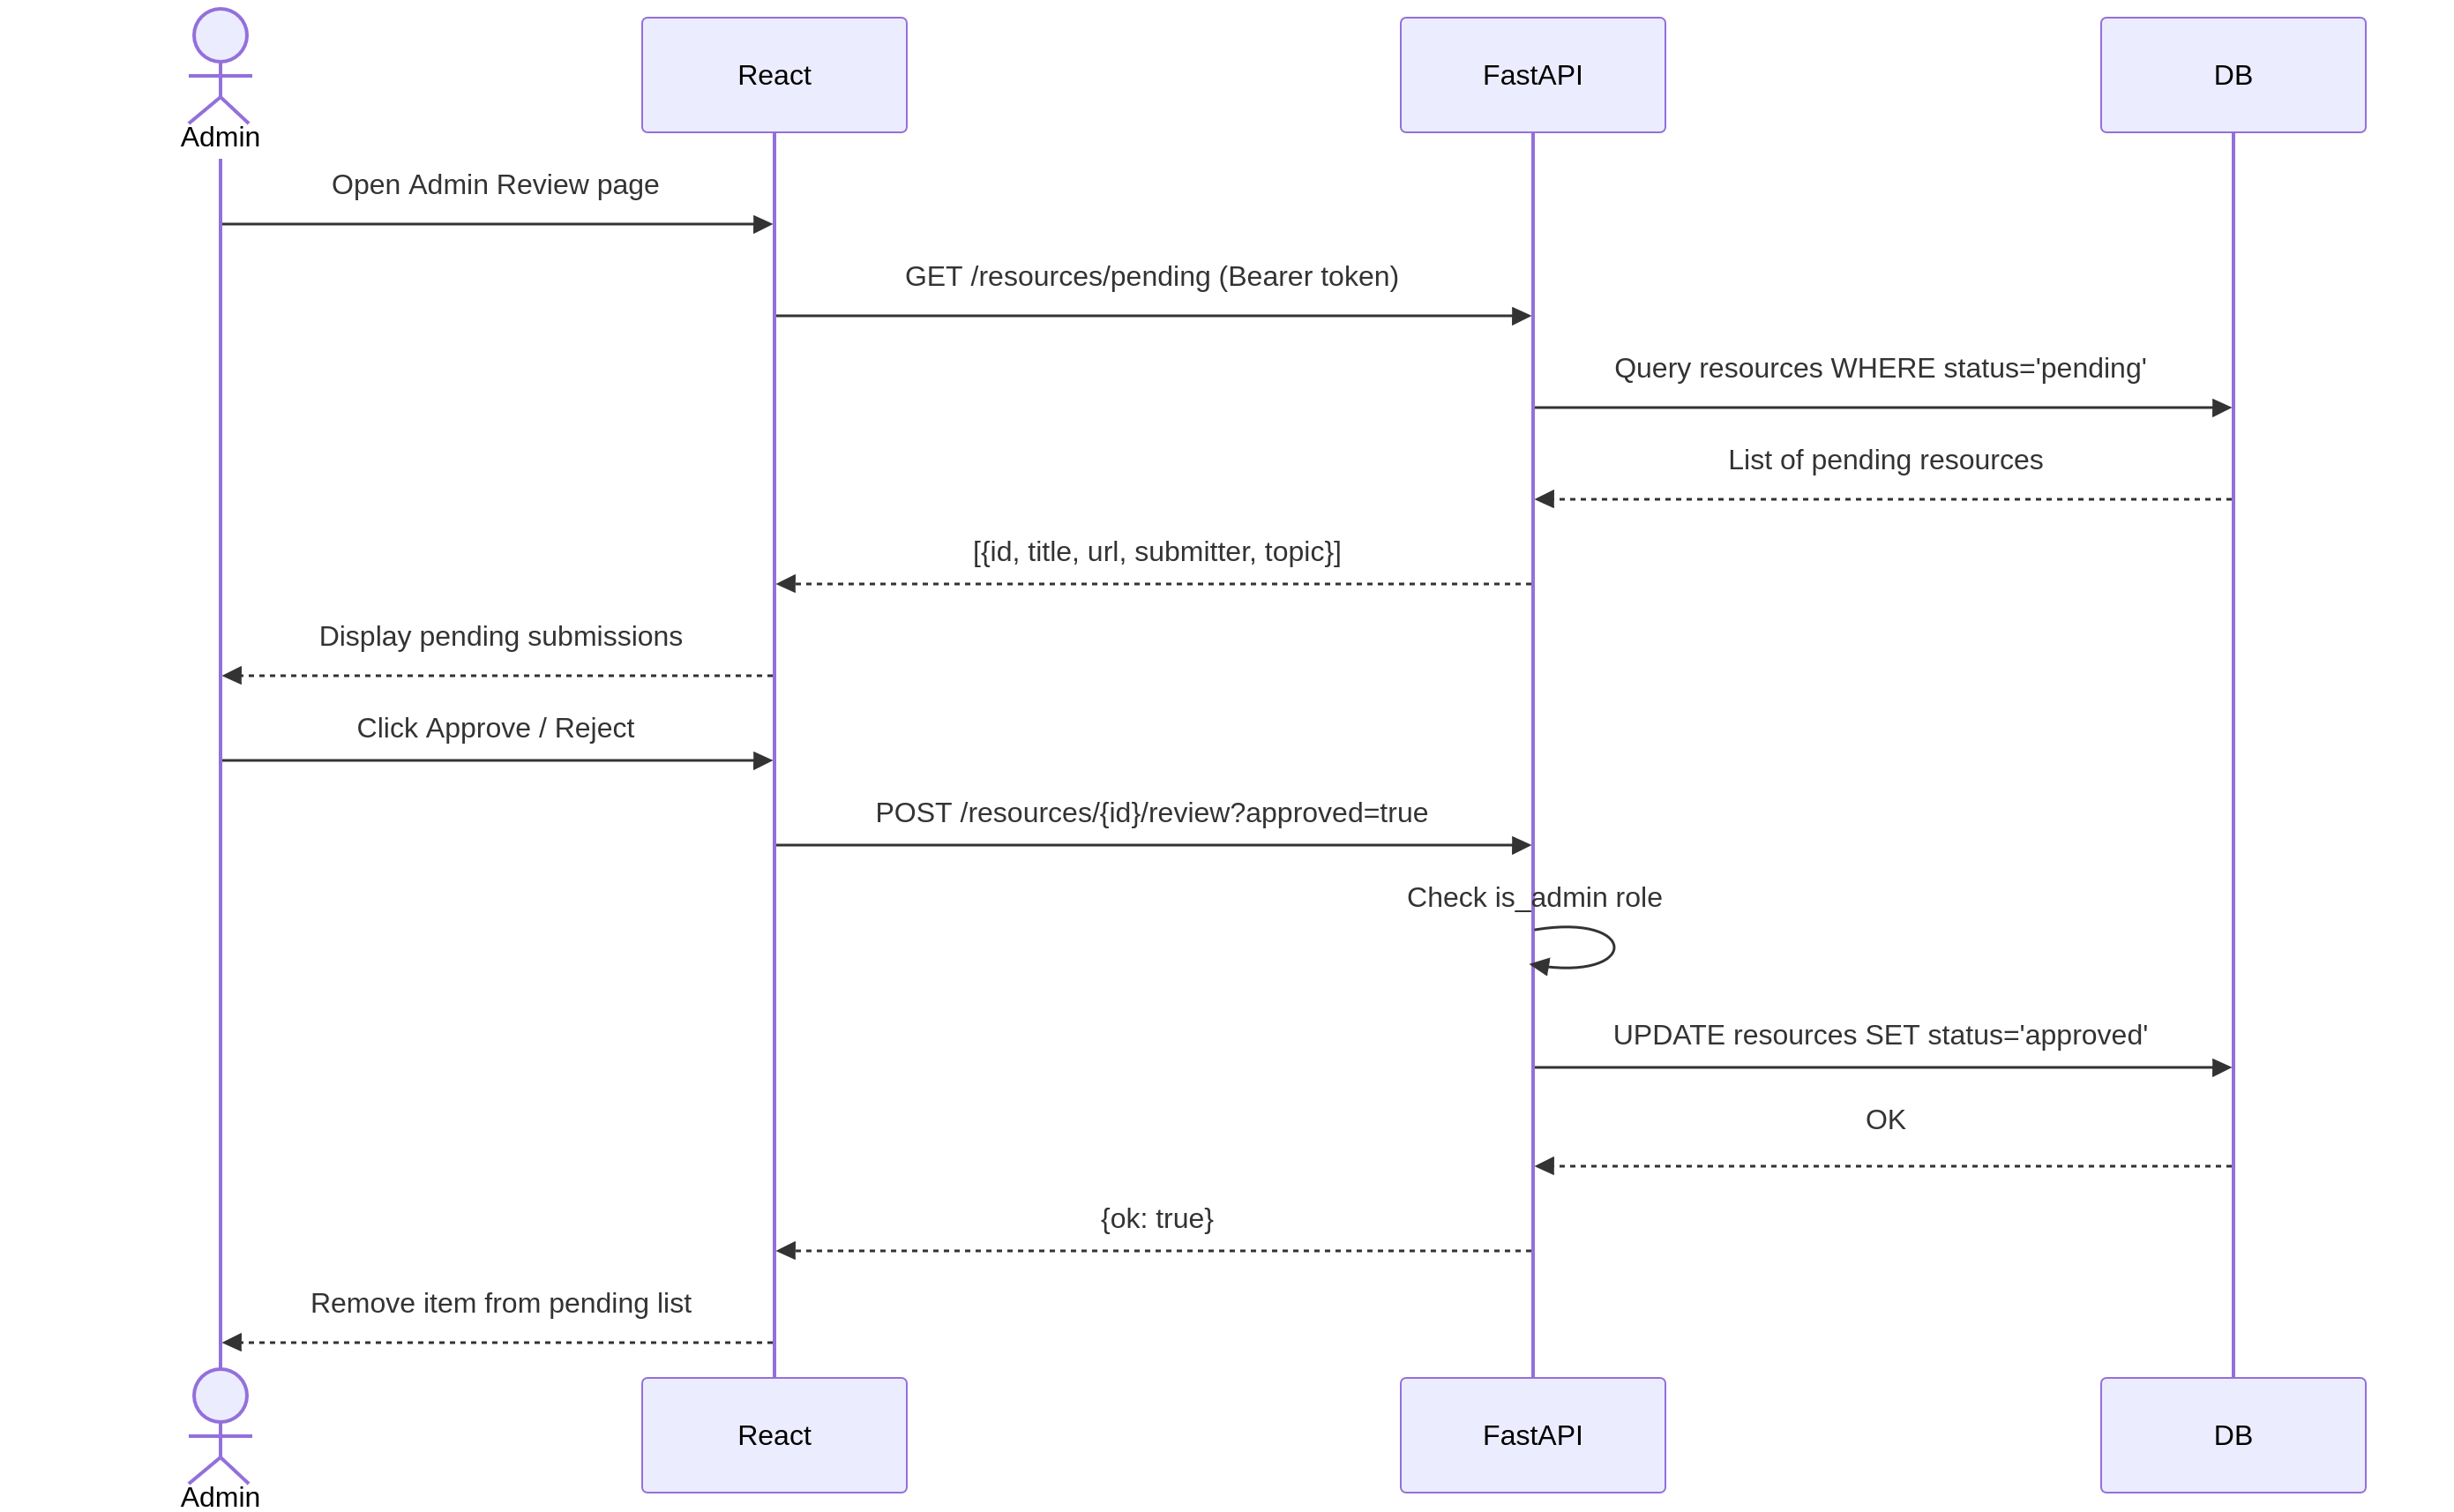
\includegraphics[width=0.75\textwidth]{seq_review.png}}{\missingfig{seq\_review.png}{Sequence Diagram -- Resource Submission and Admin Review: admin approves or rejects pending submission}}
\caption{Sequence Diagram -- Resource Submission and Admin Review}
\label{fig:seq-review}
\end{figure}

\subsection{Rating Sequence}

Figure~\ref{fig:seq-rating} shows how a user rates a resource. When a rating is submitted, the system upserts the rating row (creating it if this is the user's first rating for this resource, or updating it otherwise) and returns the updated overall Bayesian average rating for that resource.

\begin{figure}[H]
\centering
\IfFileExists{seq_rating.png}{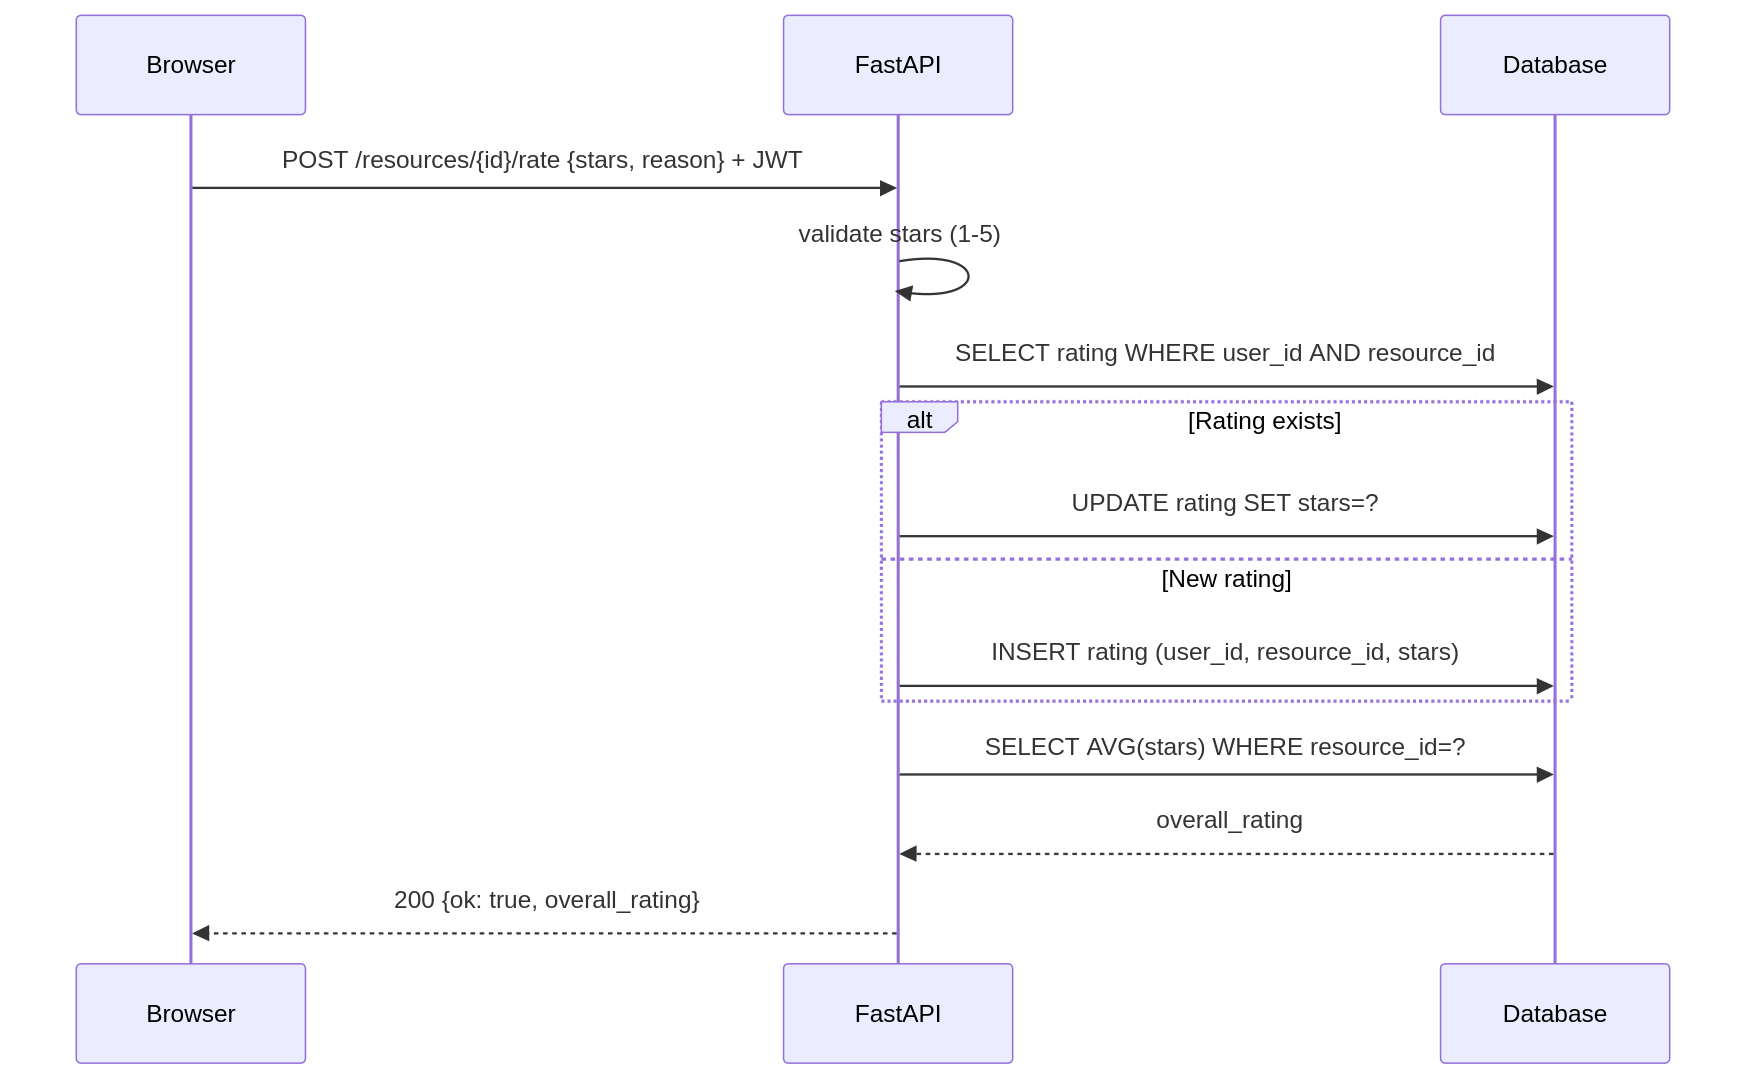
\includegraphics[width=0.75\textwidth]{seq_rating.png}}{\missingfig{seq\_rating.png}{Sequence Diagram -- Resource Rating: user submits stars → upsert rating row → compute Bayesian average → return updated score}}
\caption{Sequence Diagram -- Resource Rating with Overall Rating Update}
\label{fig:seq-rating}
\end{figure}

\section{Progress Tracking}
\label{sec:impl-progress}

Progress tracking (UC-06) is implemented at two levels. At the resource level, engagement data is recorded automatically when a user interacts with a resource. At the topic level, a user can manually mark a topic as done, which triggers an upsert on the \texttt{user\_progress} table.

\subsection{Topic Progress Sequence}

Figure~\ref{fig:seq-progress} shows how a user marks a topic as completed. The progress page also aggregates this data to show a 30-day activity heatmap, total resources completed, topics finished, and total time spent.

\begin{figure}[H]
\centering
\IfFileExists{seq_progress.png}{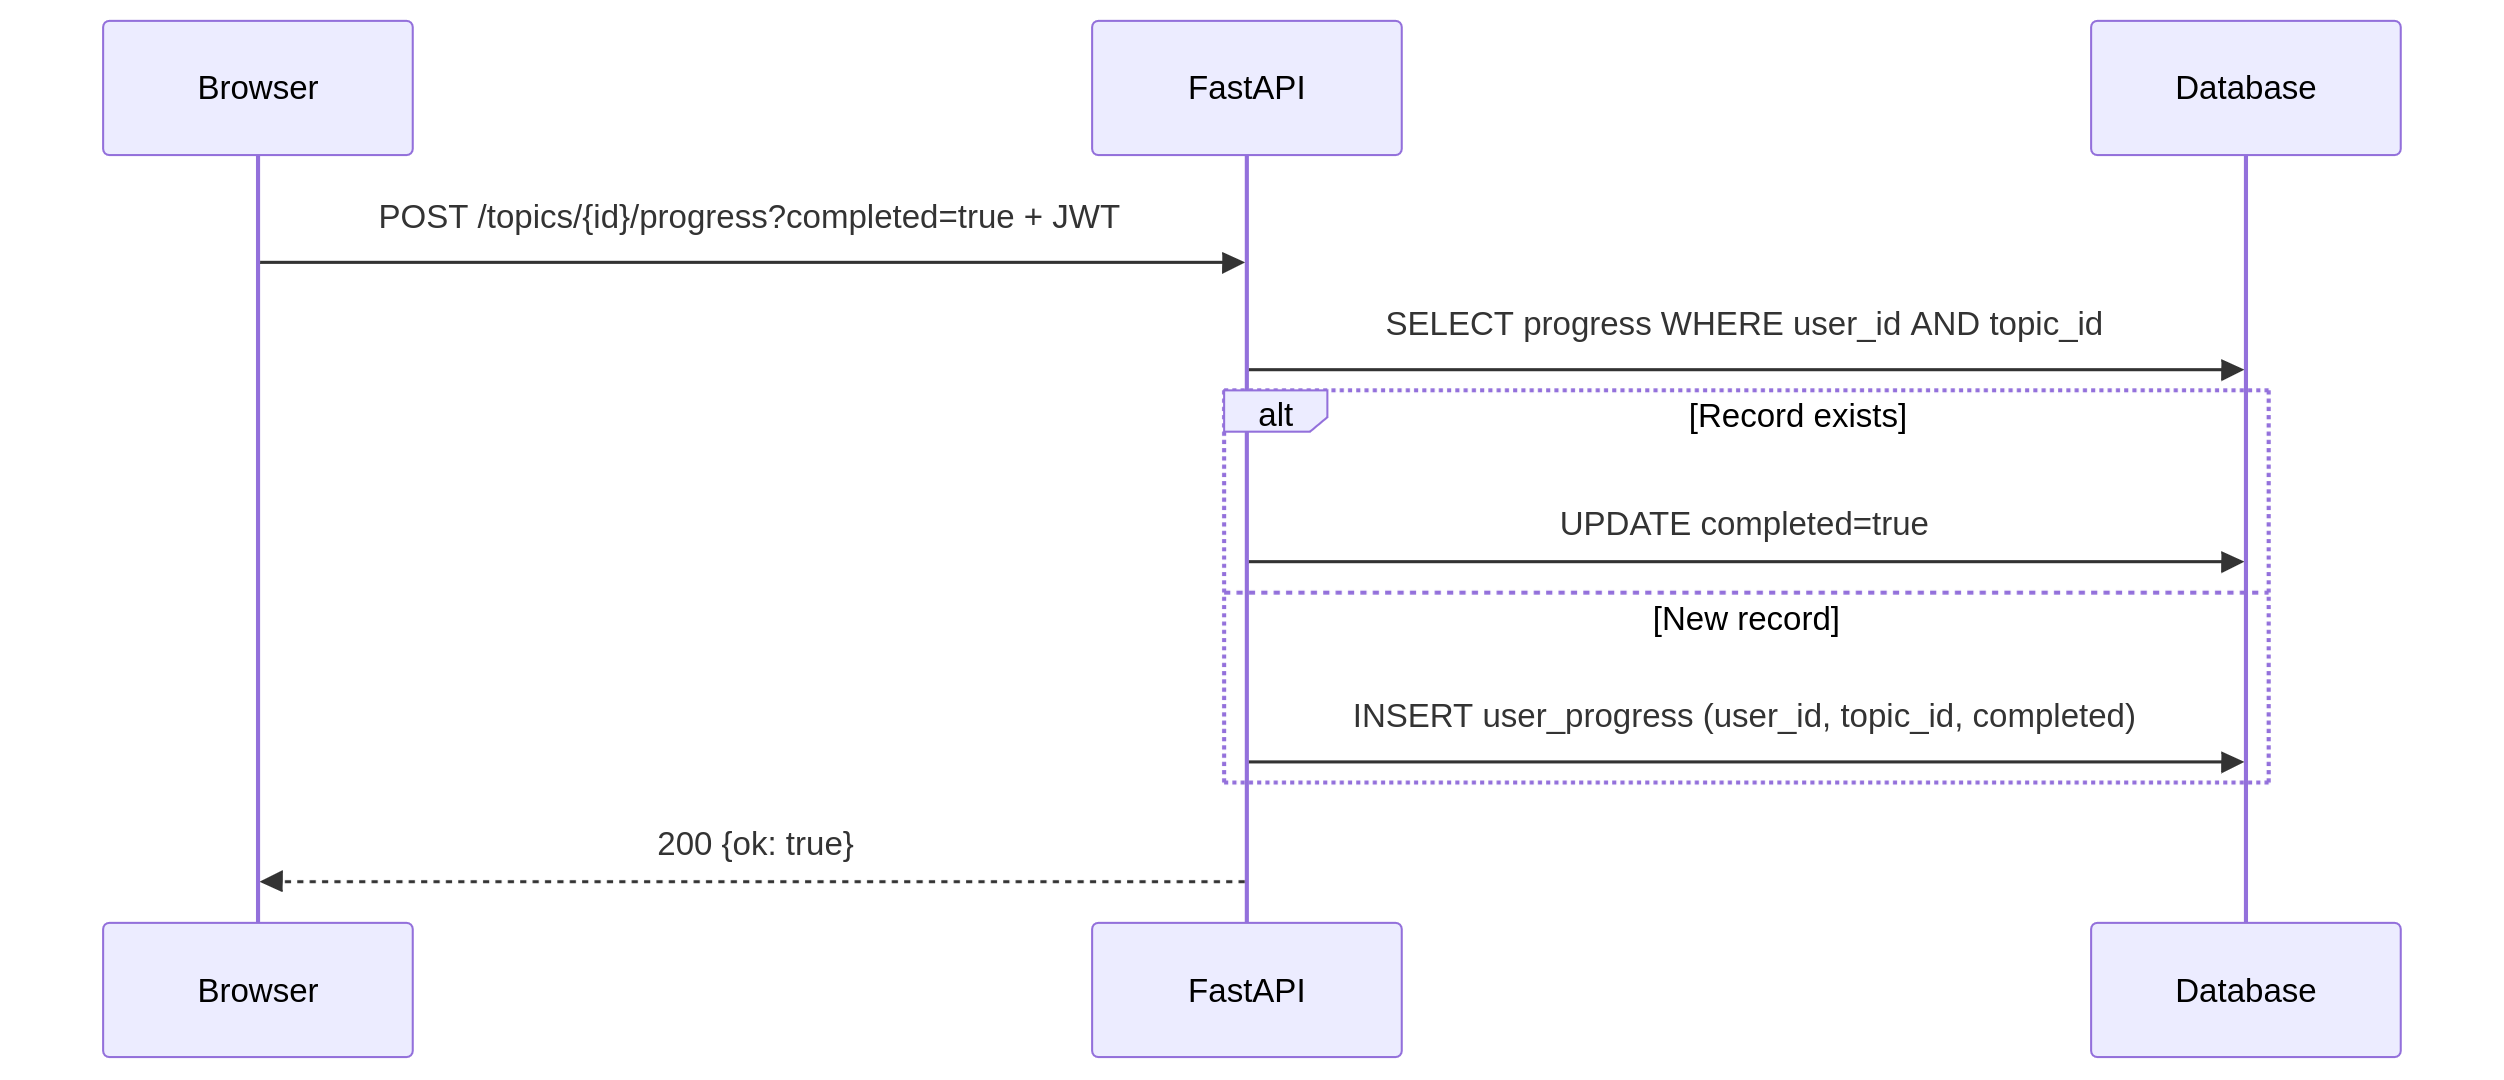
\includegraphics[width=0.75\textwidth]{seq_progress.png}}{\missingfig{seq\_progress.png}{Sequence Diagram -- Topic Progress Tracking: user clicks complete → POST /topics/\{id\}/progress → upsert user\_progress}}
\caption{Sequence Diagram -- Topic Progress Tracking}
\label{fig:seq-progress}
\end{figure}

\section{Recommendation Engine}
\label{sec:impl-rec}

The recommendation engine is the core academic contribution of this project. It combines two complementary approaches to handle both active users and cold-start users.

\subsection{Recommendation Sequence}

Figure~\ref{fig:seq-rec} shows how recommendations are generated when a user opens a topic page or the home feed. The engine runs synchronously on each request, building the user-resource matrix from live data.

\begin{figure}[H]
\centering
\IfFileExists{seq_rec.png}{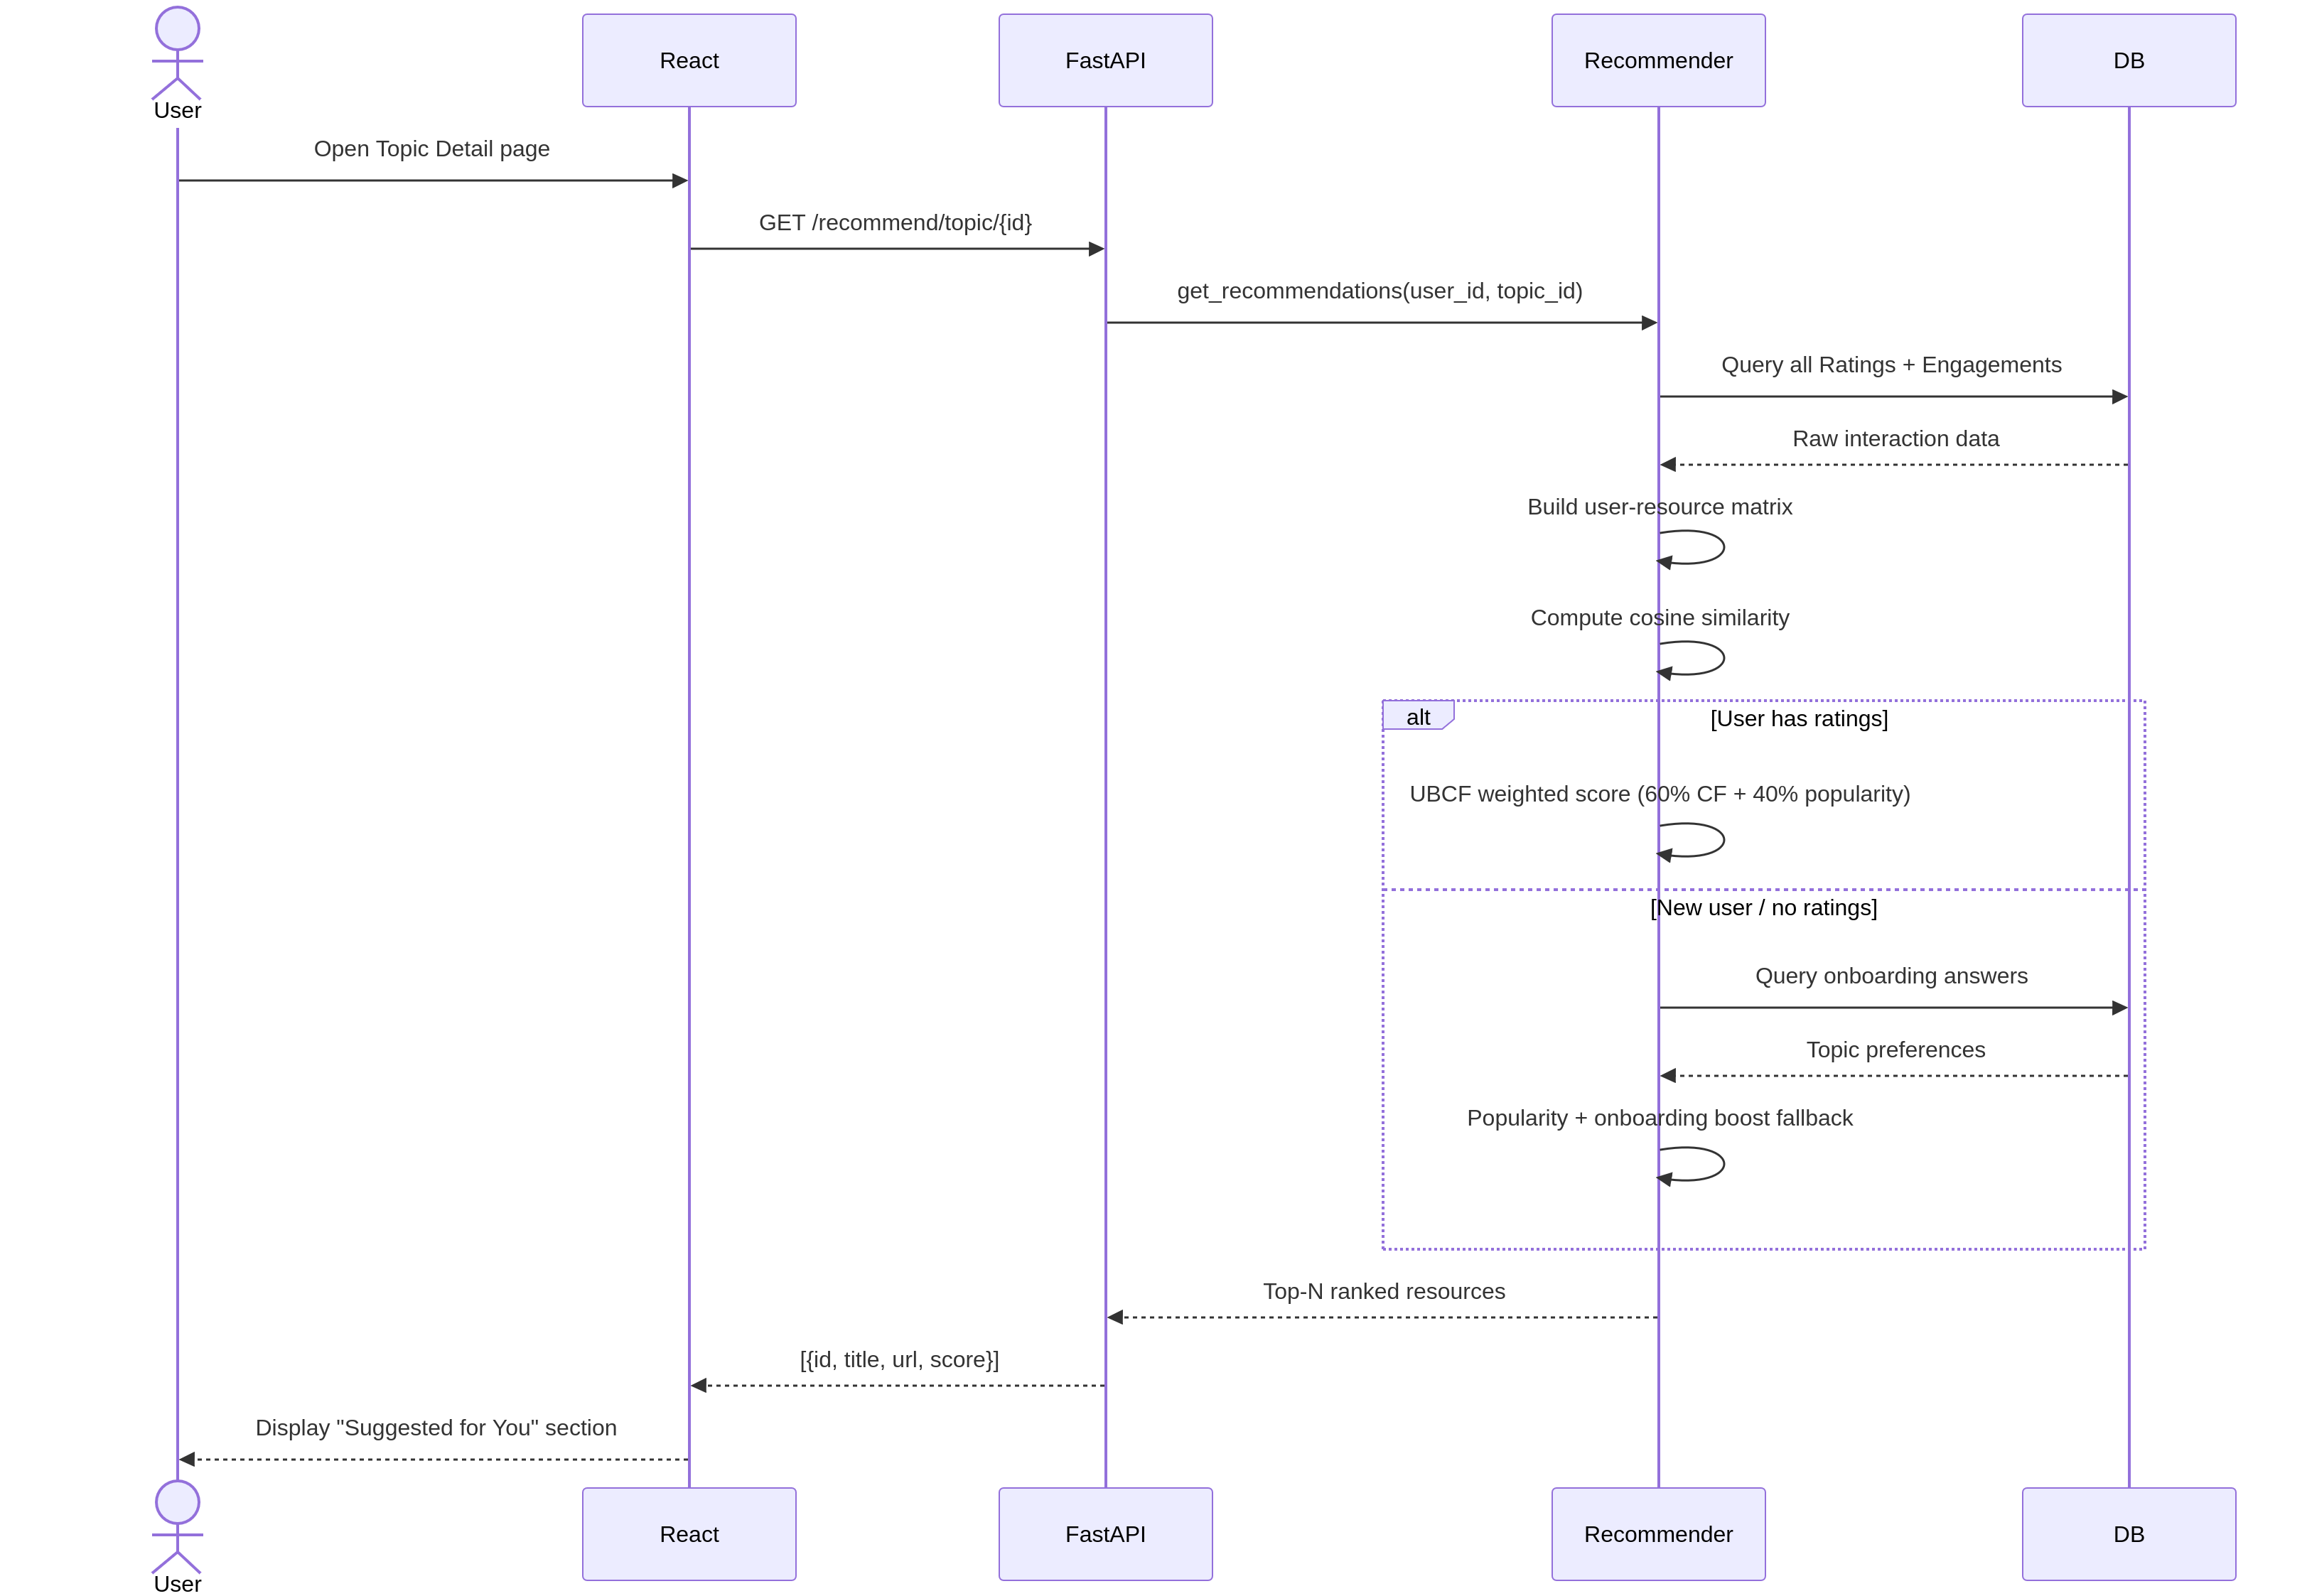
\includegraphics[width=0.85\textwidth]{seq_rec.png}}{\missingfig{seq\_rec.png}{Sequence Diagram -- Recommendation Generation: GET /recommend/\{id\} → build matrix → cosine similarity → rank → return top-N}}
\caption{Sequence Diagram -- Recommendation Generation}
\label{fig:seq-rec}
\end{figure}

\subsection{User-Based Collaborative Filtering (UBCF)}

For users who have rated at least one resource, the system builds a user-resource matrix where each cell represents a weighted engagement score. Figure~\ref{fig:ubcf-matrix} illustrates how the matrix is used to predict a missing score for the target user.

\begin{figure}[H]
\centering
\begin{tikzpicture}[
  cell/.style={draw, minimum width=1.6cm, minimum height=0.7cm, font=\small},
  header/.style={draw, minimum width=1.6cm, minimum height=0.7cm, font=\small\bfseries, fill=gray!20},
  rowlabel/.style={minimum width=1.8cm, minimum height=0.7cm, font=\small\bfseries, align=right},
  predict/.style={draw, minimum width=1.6cm, minimum height=0.7cm, font=\small\bfseries, fill=yellow!40},
  highlight/.style={draw, minimum width=1.6cm, minimum height=0.7cm, font=\small, fill=blue!10},
]

% Column headers
\node[rowlabel] (r0) at (0,0) {};
\node[header, right=0cm of r0] (h1) {Res 1};
\node[header, right=0cm of h1] (h2) {Res 2};
\node[header, right=0cm of h2] (h3) {Res 3};
\node[header, right=0cm of h3] (h4) {Res 4};
\node[header, right=0cm of h4] (h5) {Res 5};

% Row: User A
\node[rowlabel, below=0cm of r0] (rA) {User A};
\node[cell, right=0cm of rA] {0.82};
\node[cell, right=0cm of rA-|h2] {0.65};
\node[cell, right=0cm of rA-|h3] {0.00};
\node[cell, right=0cm of rA-|h4] {0.71};
\node[cell, right=0cm of rA-|h5] {0.00};

% Row: User B
\node[rowlabel, below=0cm of rA] (rB) {User B};
\node[highlight, right=0cm of rB] {0.78};
\node[cell,    right=0cm of rB-|h2] {0.60};
\node[cell,    right=0cm of rB-|h3] {0.88};
\node[highlight, right=0cm of rB-|h4] {0.00};
\node[highlight, right=0cm of rB-|h5] {0.75};

% Row: User C (target)
\node[rowlabel, below=0cm of rB] (rC) {\textbf{User C ★}};
\node[highlight, right=0cm of rC] {\textbf{0.80}};
\node[cell,    right=0cm of rC-|h2] {0.00};
\node[cell,    right=0cm of rC-|h3] {0.00};
\node[highlight, right=0cm of rC-|h4] {\textbf{0.68}};
\node[predict, right=0cm of rC-|h5] {\textbf{?}};

% Row: User D
\node[rowlabel, below=0cm of rC] (rD) {User D};
\node[cell, right=0cm of rD] {0.00};
\node[cell, right=0cm of rD-|h2] {0.55};
\node[cell, right=0cm of rD-|h3] {0.90};
\node[cell, right=0cm of rD-|h4] {0.00};
\node[cell, right=0cm of rD-|h5] {0.00};

\end{tikzpicture}
\caption{UBCF User-Resource Matrix. User C (target, ★) shares high scores on Resource 1 and 4 with User B (blue). The system predicts User C's score for Resource 5 using User B's engagement, then recommends it.}
\label{fig:ubcf-matrix}
\end{figure}

Figure~\ref{fig:score-weights} shows the five input signals and their weights that make up each cell value in the matrix.

\begin{figure}[H]
\centering
\IfFileExists{score_formula.png}{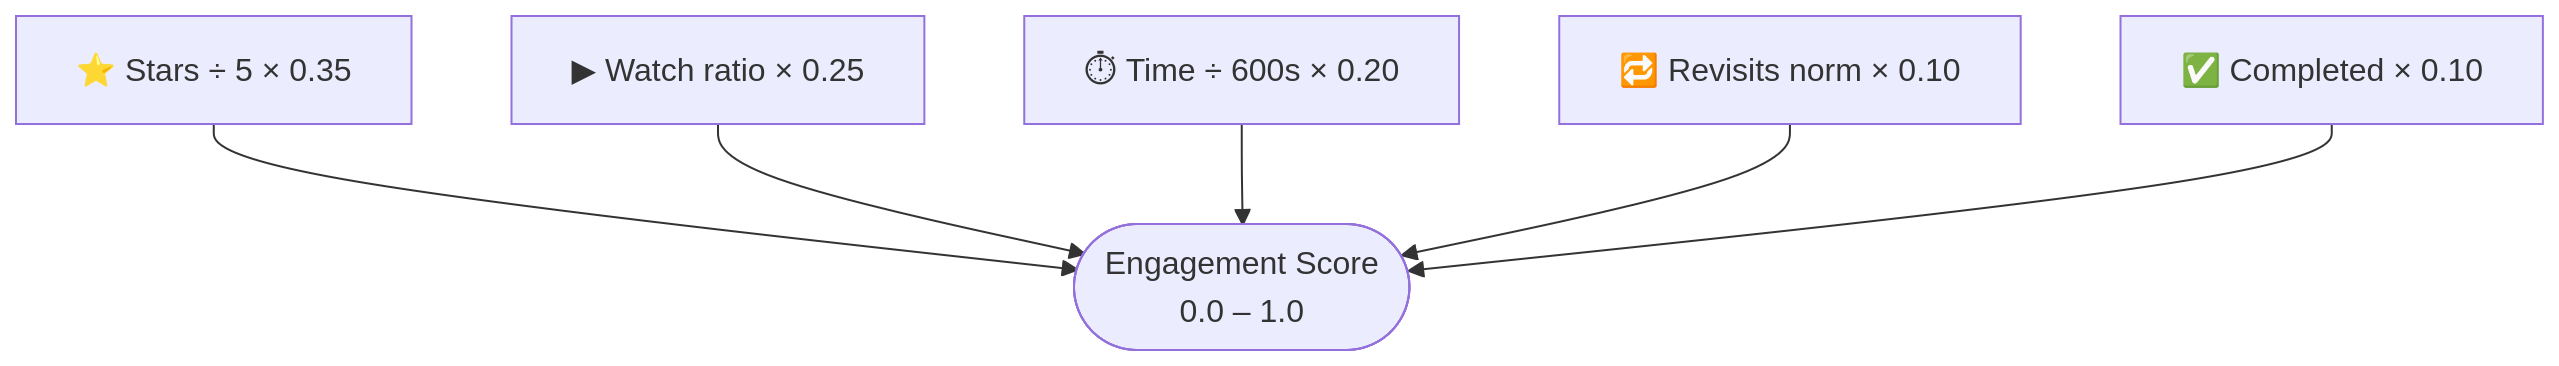
\includegraphics[width=0.72\textwidth]{score_formula.png}}{%
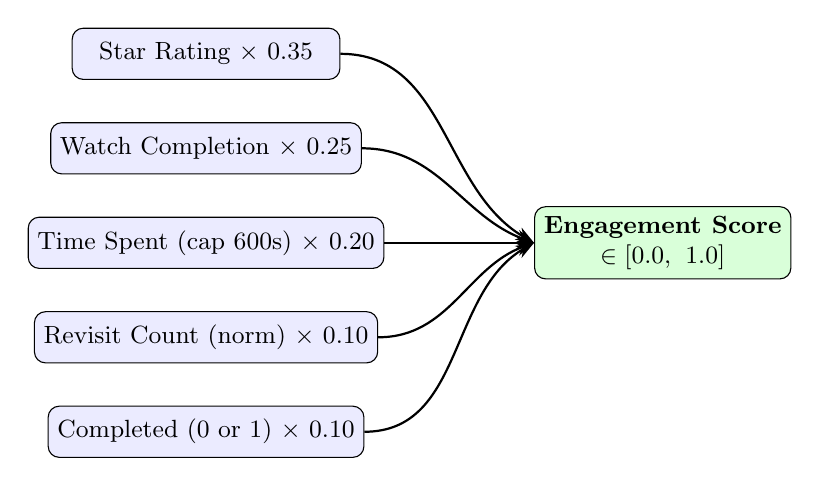
\begin{tikzpicture}[
  signal/.style={draw, rounded corners, fill=blue!8, minimum width=3.4cm, minimum height=0.65cm, font=\small, align=center},
  result/.style={draw, rounded corners, fill=green!15, minimum width=3.0cm, minimum height=0.8cm, font=\small\bfseries, align=center},
  arr/.style={-{Stealth}, thick},
]
\node[signal] (s1) at (0, 4.0)  {Star Rating $\times\ 0.35$};
\node[signal] (s2) at (0, 2.8)  {Watch Completion $\times\ 0.25$};
\node[signal] (s3) at (0, 1.6)  {Time Spent (cap 600s) $\times\ 0.20$};
\node[signal] (s4) at (0, 0.4)  {Revisit Count (norm) $\times\ 0.10$};
\node[signal] (s5) at (0, -0.8) {Completed (0 or 1) $\times\ 0.10$};
\node[result] (sc) at (5.8, 1.6){Engagement Score \\ $\in [0.0,\ 1.0]$};
\draw[arr] (s1.east) to[out=0,in=150] (sc.west);
\draw[arr] (s2.east) to[out=0,in=160] (sc.west);
\draw[arr] (s3.east) -- (sc.west);
\draw[arr] (s4.east) to[out=0,in=200] (sc.west);
\draw[arr] (s5.east) to[out=0,in=210] (sc.west);
\end{tikzpicture}}
\caption{Engagement Score -- Five Input Signals and Weights}
\label{fig:score-weights}
\end{figure}

\begin{equation}
  \text{score} = 0.35 \cdot \frac{\text{stars}}{5} + 0.25 \cdot w_{\text{watch}} + 0.20 \cdot \frac{\min(t, 600)}{600} + 0.10 \cdot r_{\text{revisit}} + 0.10 \cdot c_{\text{complete}}
\end{equation}

where $w_{\text{watch}}$ is the watch completion ratio (0--1), $t$ is time spent in seconds capped at 600, $r_{\text{revisit}}$ is a normalised revisit count, and $c_{\text{complete}}$ is 1 if the resource was marked complete. The weights were set to reflect the relative reliability of each signal: explicit star ratings carry the most weight (35\%), while completion and revisit signals serve as supporting evidence.

Cosine similarity is then computed between the target user's row vector and every other user's row:

\begin{equation}
  \text{sim}(u, v) = \frac{\mathbf{u} \cdot \mathbf{v}}{\|\mathbf{u}\| \cdot \|\mathbf{v}\|}
\end{equation}

The predicted score for a candidate resource $r$ not yet seen by user $u$ is a weighted combination of the collaborative score and a popularity baseline:

\begin{equation}
  \hat{s}(u, r) = 0.6 \cdot \frac{\sum_{v \neq u} \text{sim}(u,v) \cdot s(v,r)}{\sum_{v \neq u} |\text{sim}(u,v)|} + 0.4 \cdot p_r
\end{equation}

where $p_r$ is the Bayesian average popularity score of the resource. The 60/40 split between collaborative and popularity scores prevents the engine from over-fitting to a small number of similar users.

\subsection{Bayesian Average for Popularity}

To avoid the cold-resource problem (new resources with very few ratings appearing unrealistically high or low in rankings), a Bayesian average is used as the popularity baseline:

\begin{equation}
  \bar{r}_{\text{Bayes}} = \frac{m \cdot C + \sum_{i} r_i}{m + n}
\end{equation}

where $m = 5$ is the prior count, $C = 3.0$ is the prior mean rating, $n$ is the number of actual ratings, and $r_i$ are the individual star ratings. With these values, a resource with only one 5-star rating receives a Bayesian average of $\frac{5 \times 3 + 5}{5 + 1} \approx 3.33$ rather than 5.0, preventing it from dominating the ranking until it has collected sufficient evidence.

\subsection{Cold-Start Fallback}

When a new user has no ratings, cosine similarity cannot be computed. The system falls back to the Bayesian popularity ranking and boosts resources whose topics match the user's onboarding quiz answers:

\begin{lstlisting}[language=Python, caption=Cold-start topic boosting]
if resource.topic_id in boosted_topics:
    base_score += 1.5
\end{lstlisting}

Topics are only boosted if the user gave a positive answer to the corresponding onboarding question. Answers containing negative words (\texttt{no}, \texttt{never}, \texttt{don't}) are excluded from the boost set to avoid recommending content the user explicitly said they are not interested in.

\section{AI Knowledge Quiz}
\label{sec:impl-quiz}

When a user clicks ``Mark Complete'' on a topic (UC-11), the system calls the \texttt{GET /topics/\{id\}/quiz} endpoint, which uses the \textbf{Google Gemini 2.0 Flash} API to generate five multiple choice questions tailored to the topic's title and description. The quiz is shown in a modal before the topic is recorded as complete in the database.

\subsection{Quiz Flow}

The quiz presents one question at a time. Figure~\ref{fig:quiz-flow} shows the complete decision flow from clicking ``Mark Complete'' to topic completion.

\begin{figure}[H]
\centering
\IfFileExists{quiz_flow.png}{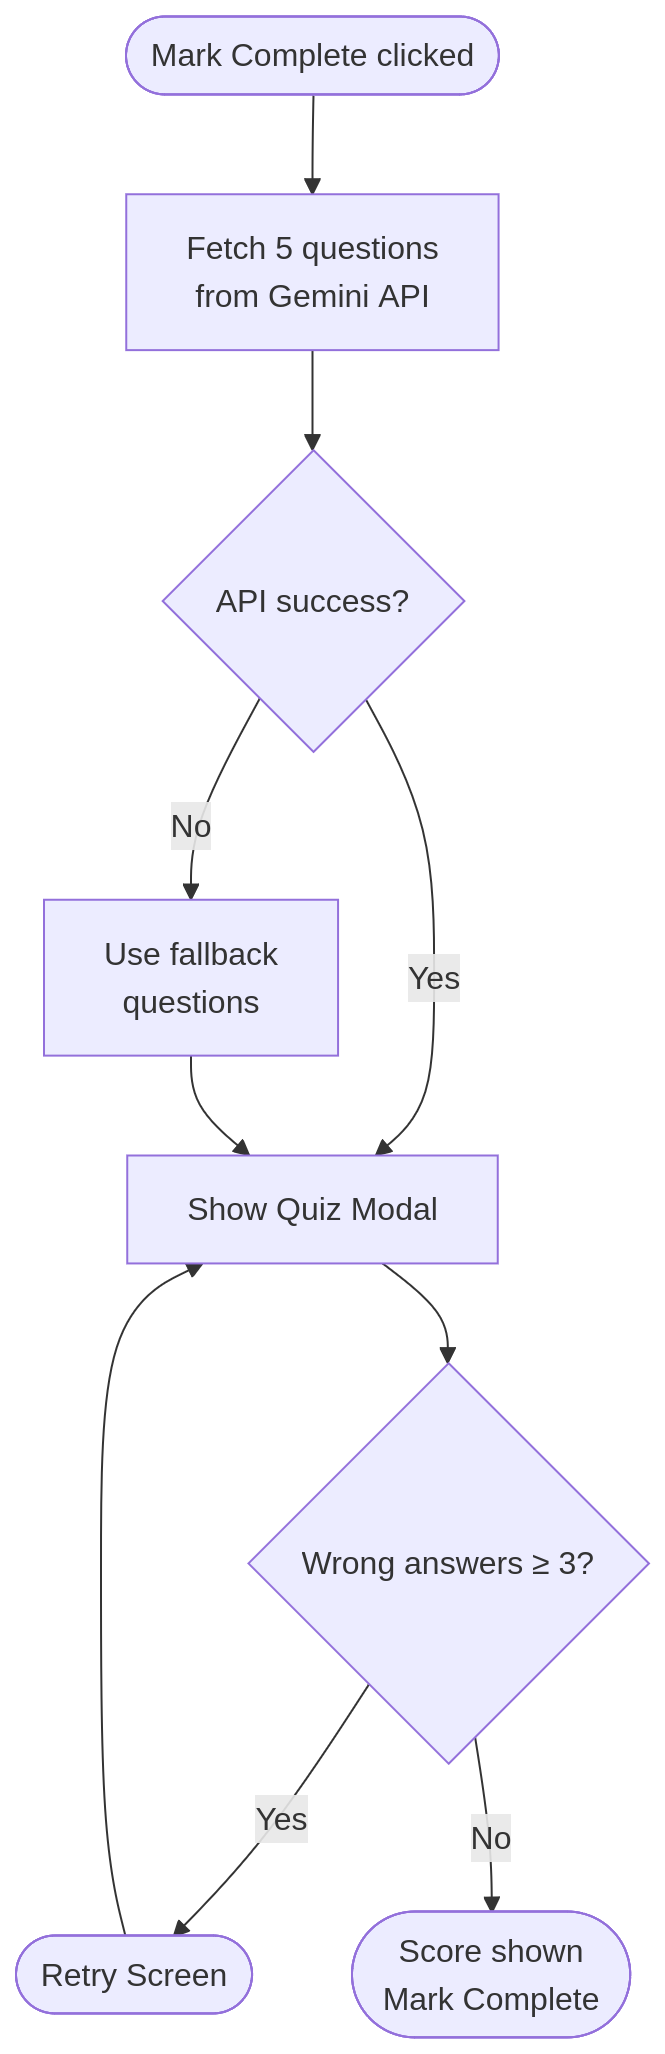
\includegraphics[width=0.38\textwidth]{quiz_flow.png}}{%
\begin{tikzpicture}[
  startstop/.style={draw, rounded corners=10pt, fill=indigo!15, minimum width=3.2cm, minimum height=0.6cm, font=\small, align=center},
  process/.style={draw, fill=blue!8, minimum width=3.2cm, minimum height=0.6cm, font=\small, align=center},
  decision/.style={draw, diamond, fill=orange!15, minimum width=1cm, font=\small, align=center, inner sep=2pt},
  arr/.style={-{Stealth}, thick},
  node distance=0.55cm,
]
\definecolor{indigo}{RGB}{79,70,229}
\node[startstop] (start)  {Mark Complete clicked};
\node[process,   below=of start]  (fetch)   {Fetch 5 questions\\ from Gemini API};
\node[decision,  below=of fetch]  (apiok)   {API OK?};
\node[process,   right=2cm of apiok] (fallback) {Use local\\ fallback Qs};
\node[process,   below=of apiok]  (quiz)    {Show Quiz Modal\\ (5 MCQ questions)};
\node[decision,  below=of quiz]   (wrong)   {Wrong $\geq 3$?};
\node[process,   right=2cm of wrong] (retry)   {Retry Screen};
\node[process,   below=of wrong]  (score)   {Show Score Summary};
\node[startstop, below=of score]  (done)    {Topic Marked Complete};
\draw[arr] (start) -- (fetch);
\draw[arr] (fetch) -- (apiok);
\draw[arr] (apiok) -- node[left,font=\small]{Yes} (quiz);
\draw[arr] (apiok) -- node[above,font=\small]{No} (fallback);
\draw[arr] (fallback) |- (quiz);
\draw[arr] (quiz) -- (wrong);
\draw[arr] (wrong) -- node[left,font=\small]{No} (score);
\draw[arr] (wrong) -- node[above,font=\small]{Yes} (retry);
\draw[arr] (retry) |- (quiz);
\draw[arr] (score) -- (done);
\end{tikzpicture}}
\caption{AI Knowledge Quiz Decision Flow}
\label{fig:quiz-flow}
\end{figure}

The quiz presents one question at a time. The user selects one of four options (A--D) and clicks Confirm to reveal whether their answer was correct (highlighted green) or wrong (highlighted red with the correct answer also shown in green). A running wrong-answer counter is visible in the modal header. If the user accumulates \textbf{three or more incorrect answers}, the quiz ends with a retry screen prompting them to review the material and attempt the quiz again. If they pass (fewer than three wrong), a score summary is shown and a ``Mark as Complete'' button finalises the topic completion. A ``Skip quiz'' button is always available for users who wish to bypass the assessment.

\subsection{Gemini Integration}

The backend sends a structured prompt to the Gemini API requesting five topic-specific multiple choice questions with plausible distractors and varied correct-answer positions. If the Gemini API is unavailable or returns malformed JSON, the endpoint falls back to locally-generated questions derived from the topic title and description. This ensures the quiz always appears and never blocks topic completion, satisfying FR-15.

\section{Admin Review Workflow}
\label{sec:impl-adminreview}

Resources submitted by users enter a \texttt{pending} state and are invisible to other learners. The admin review page (UC-08) lists all pending submissions, showing each resource's title, URL, submitter, and associated topic. An admin can approve or reject each submission by clicking the corresponding button. Only approved resources appear in topic pages.

The admin user management page (UC-09) lists all registered accounts. Admins can delete any non-admin account. A guard condition in the delete endpoint prevents accidental removal of admin accounts -- attempting to delete an admin account returns HTTP 403 with a descriptive error message.

\section{Summary}

This chapter has shown how each of the eleven use cases is realised through a combination of frontend pages, REST API endpoints, and database operations. The most technically complex components are the recommendation engine and the AI knowledge quiz. The recommendation engine requires non-trivial matrix computation; the quiz integrates an external generative AI API with a robust fallback strategy. The next chapter lists the complete set of tools and libraries that were used to build the system.

% ============================================================
% CHAPTER 7 -- TOOLS AND TECHNIQUES
% ============================================================
\chapter{Tools and Techniques}

This chapter lists the complete set of libraries, frameworks, and external services used to build and deploy Opic. Each entry is accompanied by the category it belongs to and the specific role it played in the project. The selection criteria across all categories were: active maintenance, strong documentation, and suitability for a Python/React stack on free-tier cloud infrastructure.

Table~\ref{tab:tools} provides the full inventory.

\begin{longtable}{p{0.25\textwidth} p{0.2\textwidth} p{0.45\textwidth}}
\caption{Tools and Libraries}\label{tab:tools}\\
\toprule
\textbf{Tool} & \textbf{Category} & \textbf{Purpose} \\
\midrule
\endfirsthead
\toprule
\textbf{Tool} & \textbf{Category} & \textbf{Purpose} \\
\midrule
\endhead
React 18 & Frontend framework & Component-based UI, SPA routing \cite{react} \\
Vite & Build tool & Fast dev server, optimised production build \cite{vite} \\
React Router v6 & Routing & Client-side navigation without page reloads \cite{reactrouter} \\
Axios & HTTP client & API communication with interceptors for auth token \\
Framer Motion & Animation & Subtle entrance animations on the home page \\
FastAPI & Backend framework & REST API with automatic OpenAPI docs \cite{fastapi} \\
SQLAlchemy & ORM & Database models and query abstraction \cite{sqlalchemy} \\
Pydantic & Validation & Request body validation and response serialisation \cite{pydantic} \\
python-jose & JWT & Token generation and verification \cite{ietfjwt} \\
passlib/bcrypt & Security & Password hashing \cite{passlib,provos1999} \\
aiosmtplib & Email & Async SMTP for password reset emails \cite{aiosmtplib} \\
slowapi & Rate limiting & Per-IP request rate limiting on auth endpoints \\
NumPy & Numerical computing & Matrix operations for cosine similarity \cite{numpy} \\
scikit-learn & ML utilities & Vector normalisation \cite{sklearn} \\
PostgreSQL & Database & Production relational database \cite{postgresql} \\
SQLite & Database & Development and testing database \cite{sqlite} \\
pytest + httpx & Testing & Automated API tests \\
Google Gemini API & AI & Generative AI for topic knowledge quiz \cite{gemini2024} \\
Docker Compose & Containerisation & Local full-stack development environment \cite{docker} \\
Render & Cloud hosting & Backend and database deployment \\
Vercel & CDN/hosting & Frontend deployment \\
GitHub Actions & CI & Automated test run on every push \cite{githubactions} \\
\bottomrule
\end{longtable}

The most notable dependency choices are \textbf{FastAPI} over Flask \cite{flask} (for automatic OpenAPI generation and native Pydantic integration \cite{pydantic}), \textbf{SQLAlchemy} over a raw SQL approach (for type-safe ORM models and database-agnostic queries \cite{sqlalchemy}), and \textbf{NumPy} \cite{numpy} for the recommendation matrix operations (for vectorised cosine similarity without writing low-level loops). All dependencies are pinned to specific versions in \texttt{requirements.txt} to ensure reproducible builds across development and production environments.

% ============================================================
% CHAPTER 8 -- RESULTS AND DISCUSSION
% ============================================================
\chapter{Results and Discussion}

This chapter evaluates the Opic platform against the requirements defined in Chapter 2. Section~\ref{sec:results-func} confirms the implementation status of all functional requirements. Section~\ref{sec:results-ui} analyses the key screens of the deployed interface. Section~\ref{sec:results-eval} discusses the system-level evaluation, including the recommendation quality test. Section~\ref{sec:results-bugs} documents the significant bugs discovered and resolved during the evaluation phase.

\section{Functional Outcomes}
\label{sec:results-func}

All fourteen functional requirements listed in Chapter 2 were implemented and verified on the live deployment at \url{https://final-project-git-main-lamawds-projects.vercel.app}. Table~\ref{tab:results} summarises the implementation status of each requirement.

\begin{longtable}{p{0.1\textwidth} p{0.5\textwidth} p{0.25\textwidth}}
\caption{Functional Requirements Implementation Status}\label{tab:results}\\
\toprule
\textbf{ID} & \textbf{Requirement} & \textbf{Status} \\
\midrule
FR-01 & User Registration & \textcolor{green!60!black}{Implemented} \\
FR-02 & User Login & \textcolor{green!60!black}{Implemented} \\
FR-03 & Password Reset & \textcolor{green!60!black}{Implemented} \\
FR-04 & Topic Browsing & \textcolor{green!60!black}{Implemented} \\
FR-05 & Resource Access & \textcolor{green!60!black}{Implemented} \\
FR-06 & Resource Submission & \textcolor{green!60!black}{Implemented} \\
FR-07 & Resource Rating & \textcolor{green!60!black}{Implemented} \\
FR-08 & Engagement Tracking & \textcolor{green!60!black}{Implemented} \\
FR-09 & Topic Progress & \textcolor{green!60!black}{Implemented} \\
FR-10 & Onboarding Quiz & \textcolor{green!60!black}{Implemented} \\
FR-11 & Recommendations & \textcolor{green!60!black}{Implemented} \\
FR-12 & Admin Review & \textcolor{green!60!black}{Implemented} \\
FR-13 & Admin User Management & \textcolor{green!60!black}{Implemented} \\
FR-14 & Home Feed & \textcolor{green!60!black}{Implemented} \\
FR-15 & AI Knowledge Quiz & \textcolor{green!60!black}{Implemented} \\
\bottomrule
\end{longtable}

The table confirms a 100\% implementation rate across all requirements. The following sections provide evidence for this claim through UI screenshots and a discussion of the recommendation quality test.

\section{User Interface Analysis}
\label{sec:results-ui}

This section presents screenshots of the main screens of the deployed platform and analyses how each screen satisfies its corresponding functional requirements.

\subsection{Login and Register}

Figure~\ref{fig:ui-login} shows the login page. The form provides specific, per-field error messages: if the email is not found in the system, the message reads ``No account found with that email''; if the password is wrong, it reads ``Incorrect password''. The register page similarly validates each field inline before hitting the server.

\begin{figure}[H]
\centering
\IfFileExists{ui_login.png}{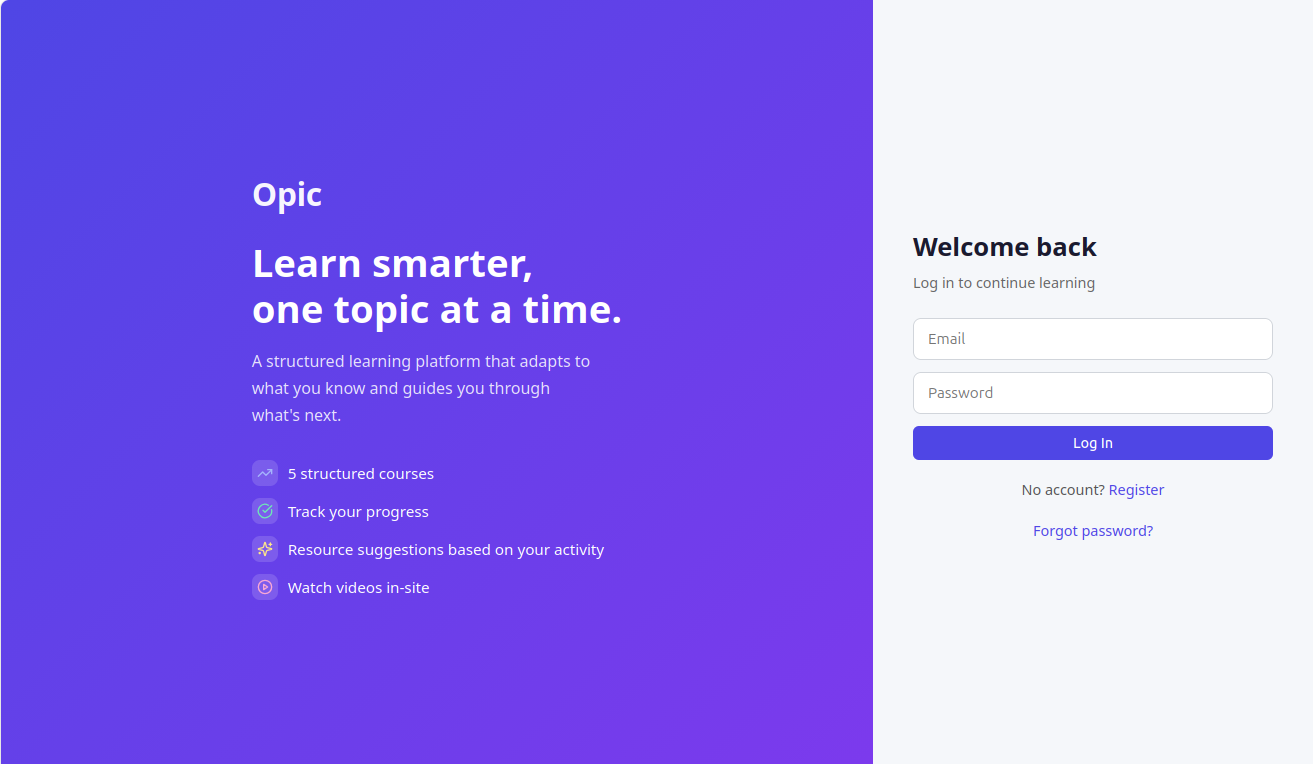
\includegraphics[width=0.85\textwidth]{ui_login.png}}{\missingfig{ui\_login.png}{Screenshot of the login page with hero branding and per-field error messages}}
\caption{Login Page -- Authentication with Specific Error Messages (FR-02)}
\label{fig:ui-login}
\end{figure}

\begin{figure}[H]
\centering
\IfFileExists{ui_register.png}{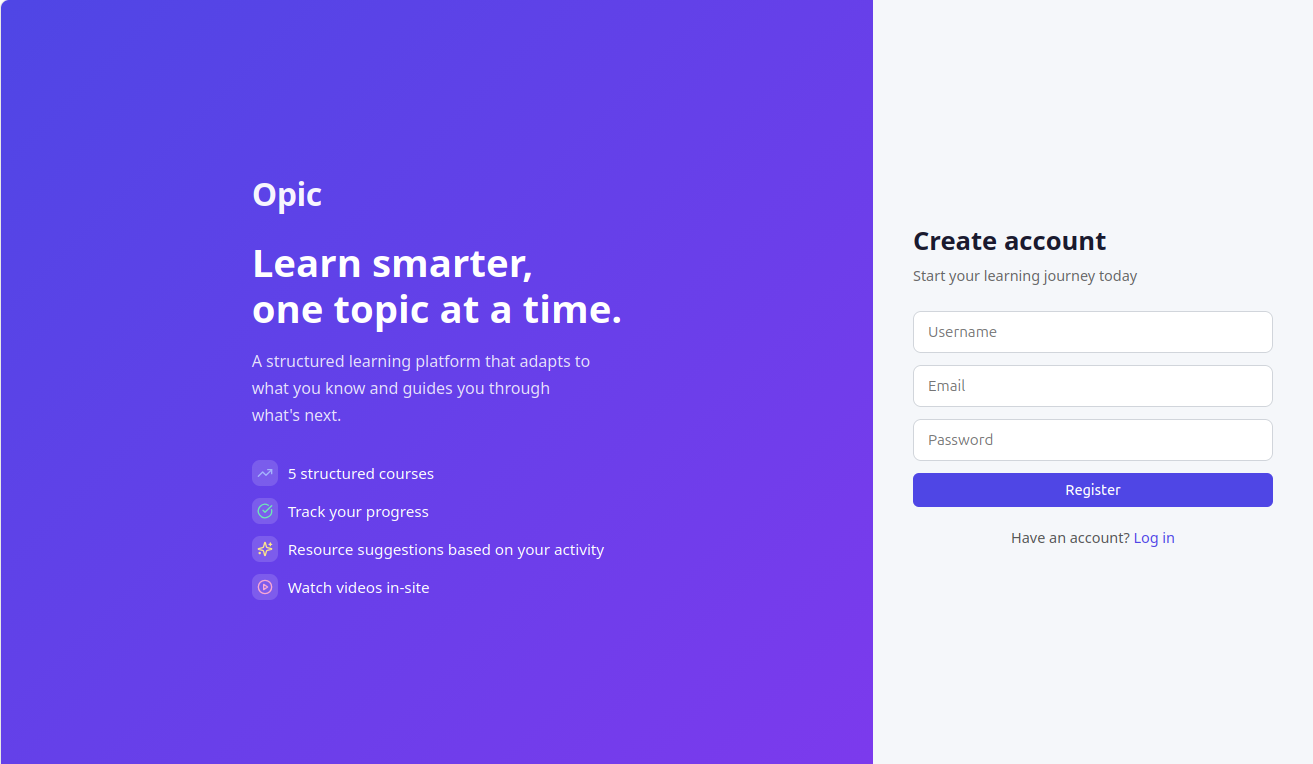
\includegraphics[width=0.85\textwidth]{ui_register.png}}{\missingfig{ui\_register.png}{Screenshot of the registration page with per-field validation}}
\caption{Registration Page -- Account Creation with Inline Validation (FR-01)}
\label{fig:ui-register}
\end{figure}

\subsection{AI Knowledge Quiz}

Figure~\ref{fig:ui-quiz} shows the AI-generated knowledge quiz modal that appears when a user clicks ``Mark Complete'' on a topic. The quiz presents five multiple choice questions generated by the Gemini API, one at a time. Correct answers are highlighted in green and wrong answers in red. If the user gets three or more questions wrong, they are prompted to retry (FR-15).

\begin{figure}[H]
\centering
\IfFileExists{ui_topic.png}{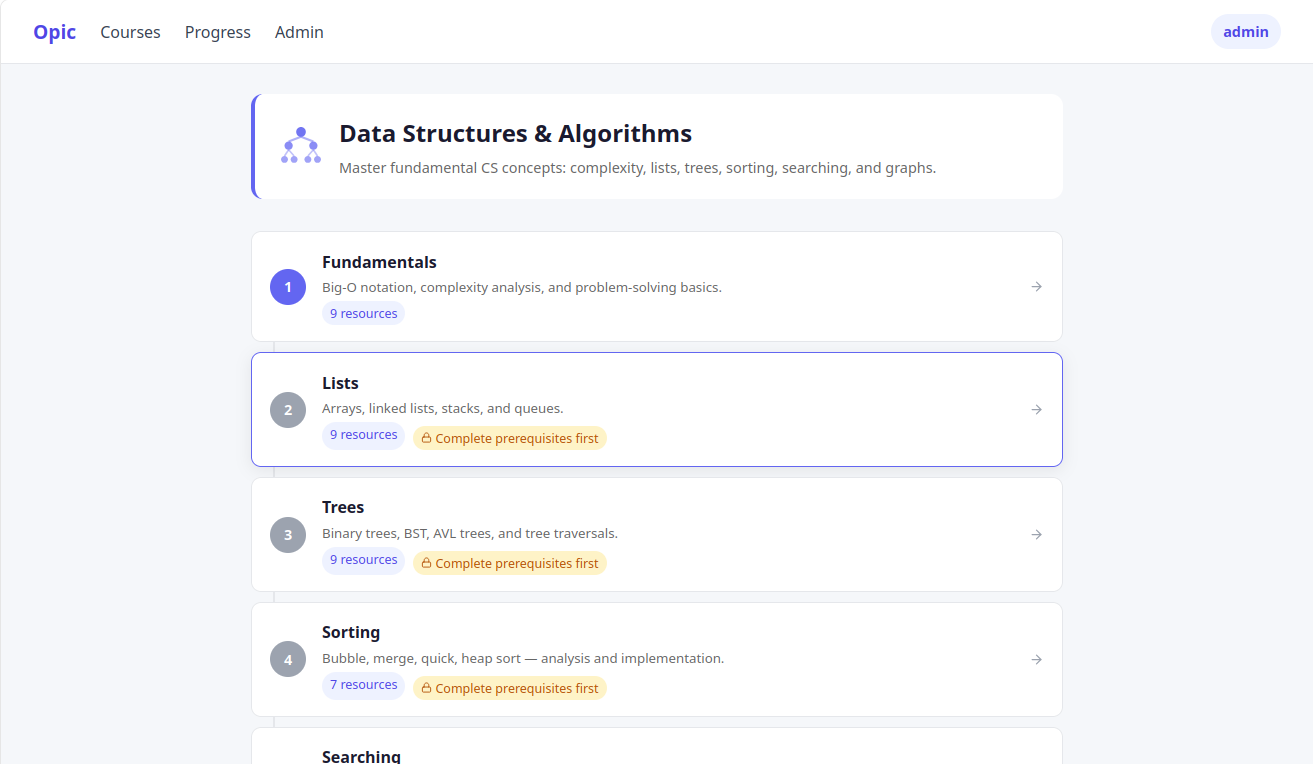
\includegraphics[width=0.85\textwidth]{ui_topic.png}}{\missingfig{ui\_topic.png}{Screenshot of the AI knowledge quiz modal showing a multiple choice question with colour-coded feedback}}
\caption{AI Knowledge Quiz -- Topic Completion Assessment (FR-15)}
\label{fig:ui-quiz}
\end{figure}

\subsection{Suggested Resources}

Figure~\ref{fig:ui-suggested} shows the personalised resource suggestions section on the topic detail page. Resources are ranked by the recommendation engine score and displayed below the topic's own resource list.

\begin{figure}[H]
\centering
\IfFileExists{ui_sugested.png}{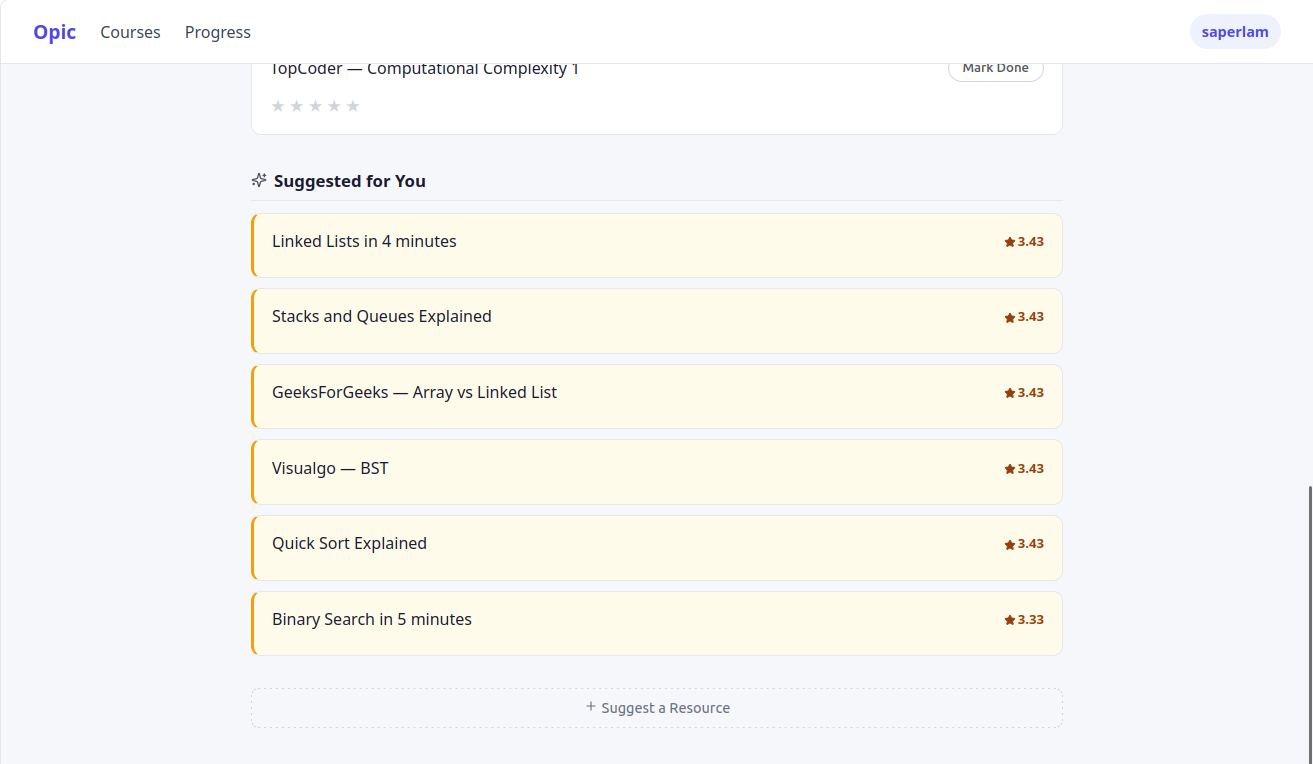
\includegraphics[width=0.85\textwidth]{ui_sugested.png}}{\missingfig{ui\_sugested.png}{Screenshot of suggested resources section on the topic detail page}}
\caption{Suggested Resources -- Collaborative Filtering Recommendations (FR-11)}
\label{fig:ui-suggested}
\end{figure}

\subsection{Home Feed}

Figure~\ref{fig:ui-home} shows the home feed page. The page is divided into two sections: a personalised ``Picks for You'' section (FR-11, FR-14) that shows the top recommended resources based on the user's interaction history, and a ``Featured This Week'' section that highlights a manually curated resource. For new users, the picks section is populated by the cold-start fallback using onboarding quiz answers (FR-10).

\begin{figure}[H]
\centering
\IfFileExists{ui_home1.png}{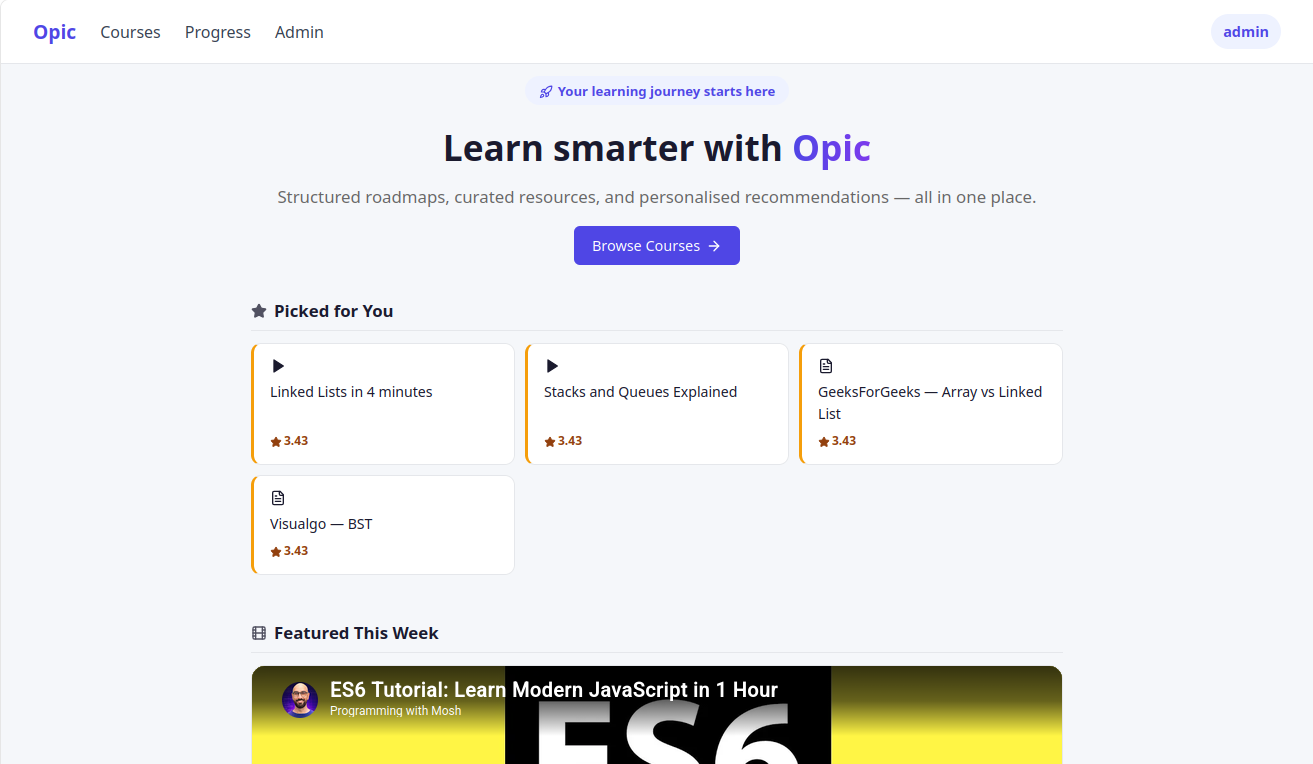
\includegraphics[width=0.9\textwidth]{ui_home1.png}}{\missingfig{ui\_home1.png}{Screenshot of the Opic home feed page showing personalised recommendations and featured video}}
\caption{Home Feed -- Personalised Recommendations and Hero (FR-11, FR-14)}
\label{fig:ui-home}
\end{figure}

\begin{figure}[H]
\centering
\IfFileExists{ui_home2.png}{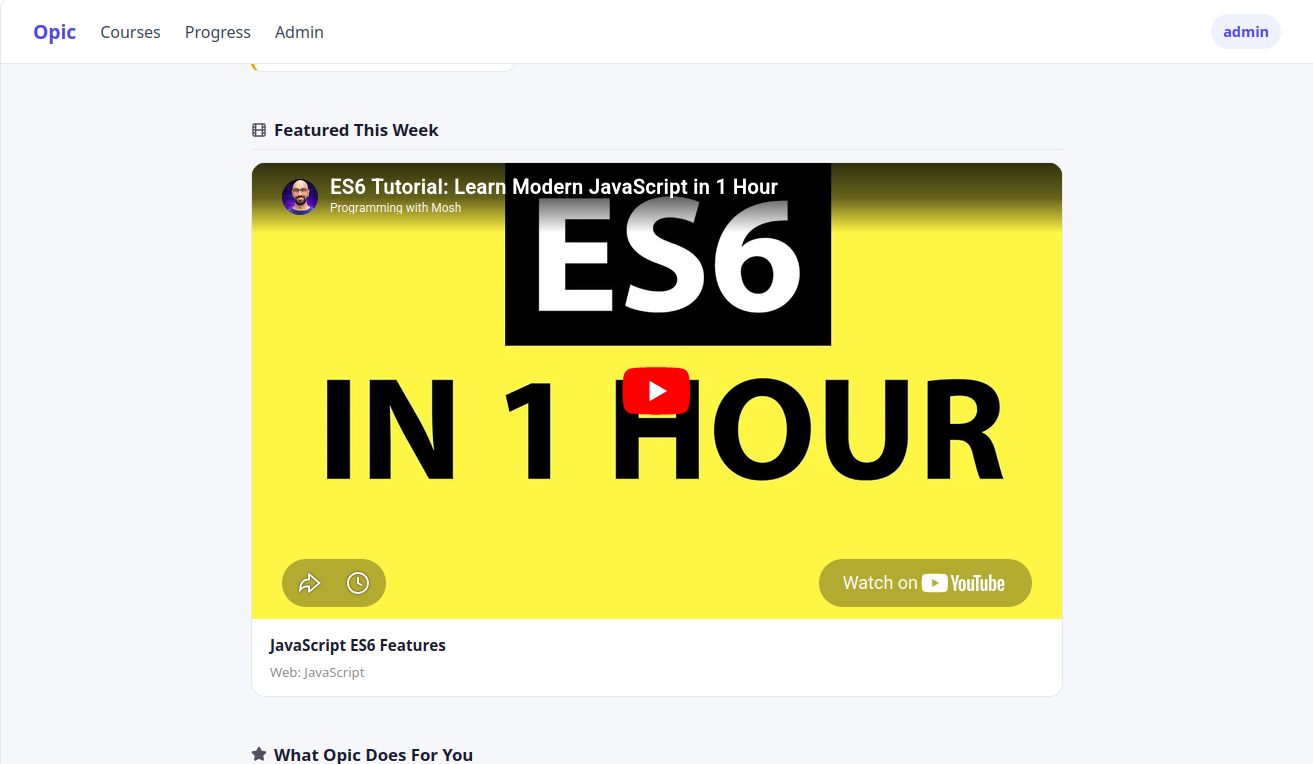
\includegraphics[width=0.9\textwidth]{ui_home2.png}}{\missingfig{ui\_home2.png}{Screenshot of the Opic home feed page lower section with features and testimonials}}
\caption{Home Feed -- Features Grid and Testimonials (FR-14)}
\label{fig:ui-home2}
\end{figure}

\subsection{Topic List and Topic Detail}

Figure~\ref{fig:ui-topics} shows the topic list page, where all topics are grouped by course and displayed in order. Prerequisite relationships are visible as dependency indicators, addressing FR-04.

\begin{figure}[H]
\centering
\IfFileExists{ui_courses.png}{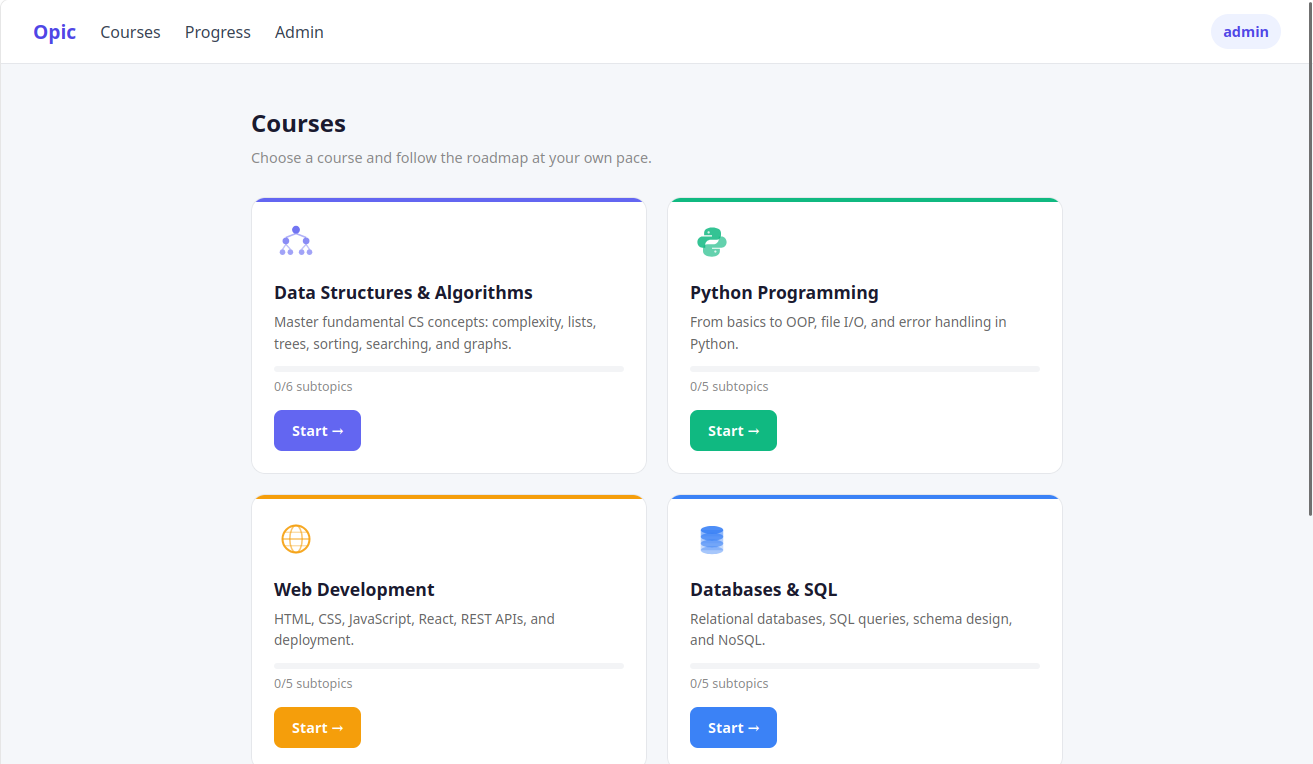
\includegraphics[width=0.9\textwidth]{ui_courses.png}}{\missingfig{ui\_courses.png}{Screenshot of the topic list page showing topics grouped by course with prerequisite indicators}}
\caption{Topic List Page -- Structured Learning Roadmap (FR-04)}
\label{fig:ui-topics}
\end{figure}

Figure~\ref{fig:ui-topic-detail} shows the topic detail page. The page lists all approved resources for the selected topic (FR-05), each with a star rating widget (FR-07) and an engagement tracking button. A ``Mark as Complete'' button at the top allows the user to update their progress (FR-09).

\begin{figure}[H]
\centering
\IfFileExists{ui_topic_details.png}{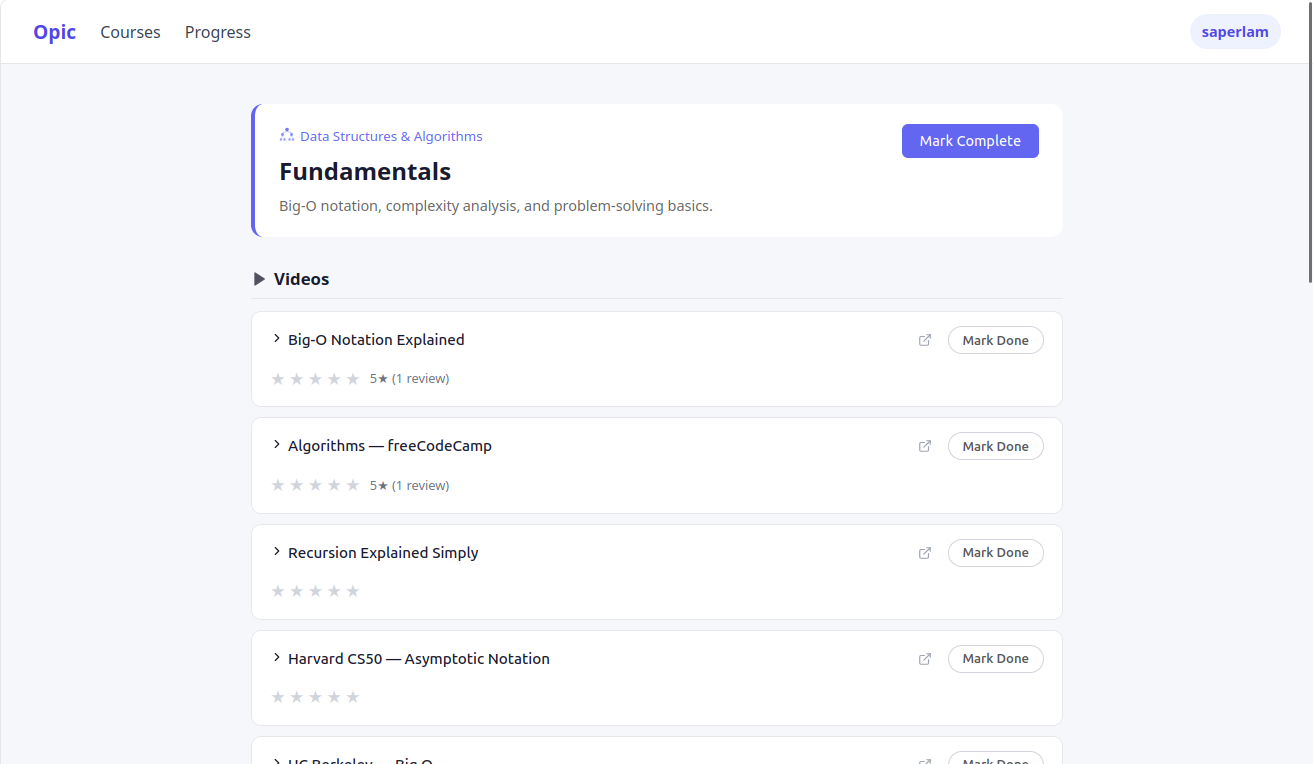
\includegraphics[width=0.9\textwidth]{ui_topic_details.png}}{\missingfig{ui\_topic\_details.png}{Screenshot of the topic detail page showing approved resources with star ratings and mark-complete button}}
\caption{Topic Detail Page -- Resources, Ratings, and Progress (FR-05, FR-07, FR-09)}
\label{fig:ui-topic-detail}
\end{figure}

\subsection{Resource Submission and Admin Review}

Figure~\ref{fig:ui-submit} shows the resource submission form that any logged-in user can access from a topic detail page. The form requires a title, URL, and resource type (video or article), satisfying FR-06.

\begin{figure}[H]
\centering
\IfFileExists{ui_submit1.png}{
\includegraphics[width=0.75\textwidth]{ui_submit1.png}}{\missingfig{ui\_submit1.png}{Screenshot of the resource submission form with title, URL, and type fields}}
\caption{Resource Submission Form -- Single Row (FR-06)}
\label{fig:ui-submit}
\end{figure}

\begin{figure}[H]
\centering
\IfFileExists{ui_submit2.png}{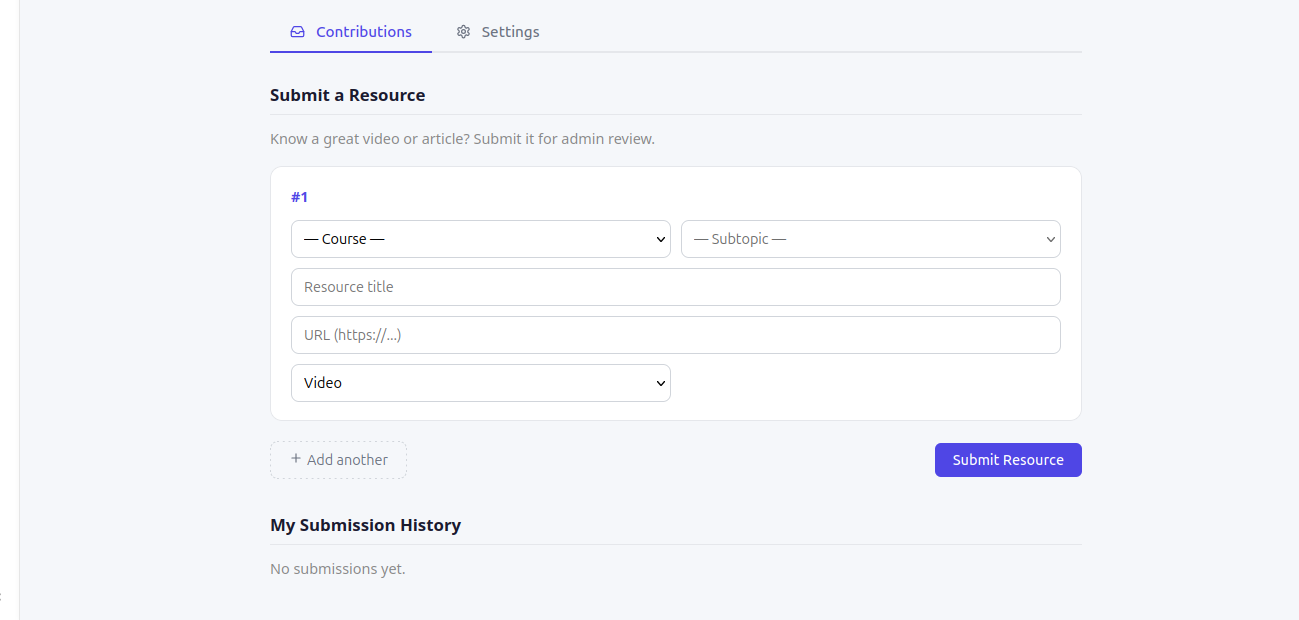
\includegraphics[width=0.9\textwidth]{ui_submit2.png}}{\missingfig{ui\_submit2.png}{Screenshot of the multi-row resource submission form in the user profile}}
\caption{Resource Submission Form -- Batch Submission via User Profile (FR-06)}
\label{fig:ui-submit2}
\end{figure}

Figure~\ref{fig:ui-admin-review} shows the admin review page. Each pending submission is displayed with its title, URL, submitter username, and associated topic. The Approve and Reject buttons trigger the review endpoint (FR-12).

\begin{figure}[H]
\centering
\IfFileExists{ui_admin_review.png}{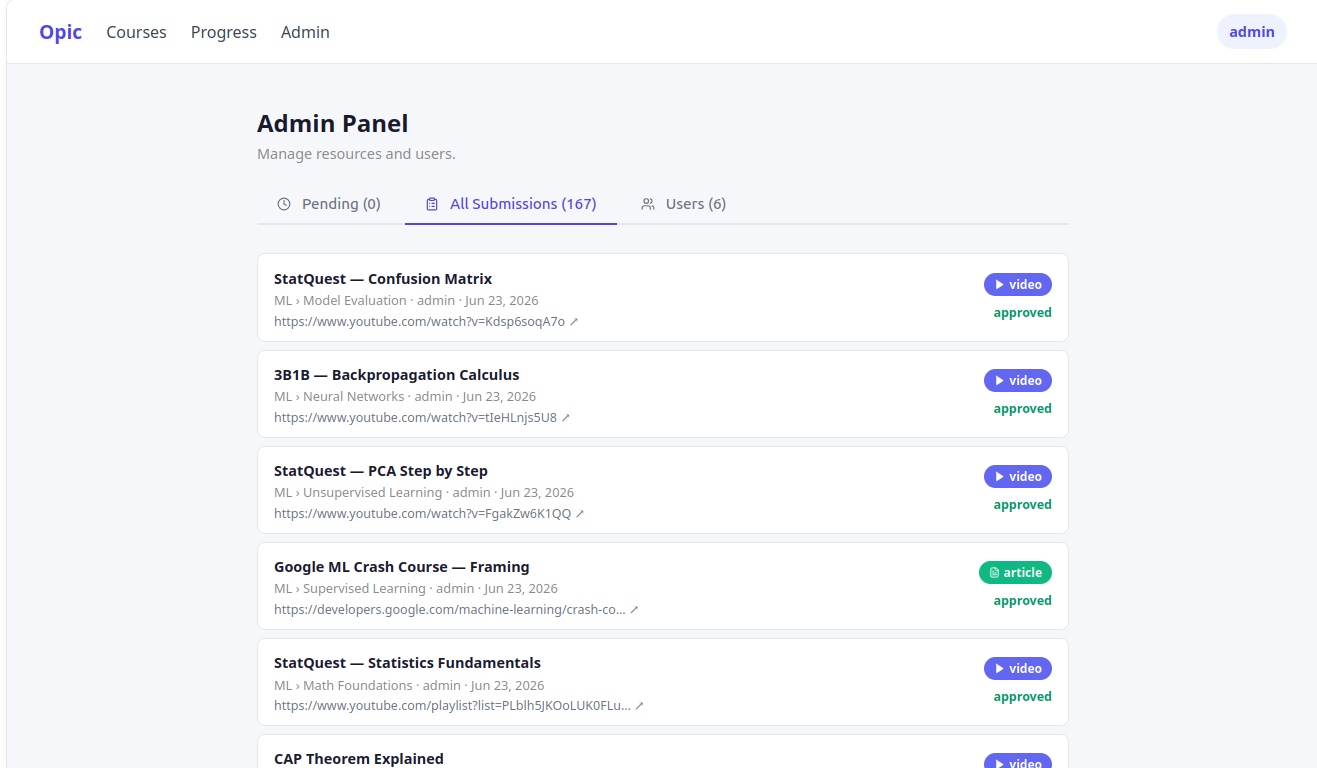
\includegraphics[width=0.9\textwidth]{ui_admin_review.png}}{\missingfig{ui\_admin\_review.png}{Screenshot of the admin review page listing pending submissions with approve/reject buttons}}
\caption{Admin Review Page -- Content Moderation (FR-12)}
\label{fig:ui-admin-review}
\end{figure}

\subsection{Progress Tracking}

Figure~\ref{fig:ui-progress} shows the progress page, which displays a 30-day activity heatmap, total resources completed, topics finished, and total time spent learning. This page addresses FR-09 and FR-08 by surfacing the engagement data collected in the background.

\begin{figure}[H]
\centering
\IfFileExists{ui_progress.png}{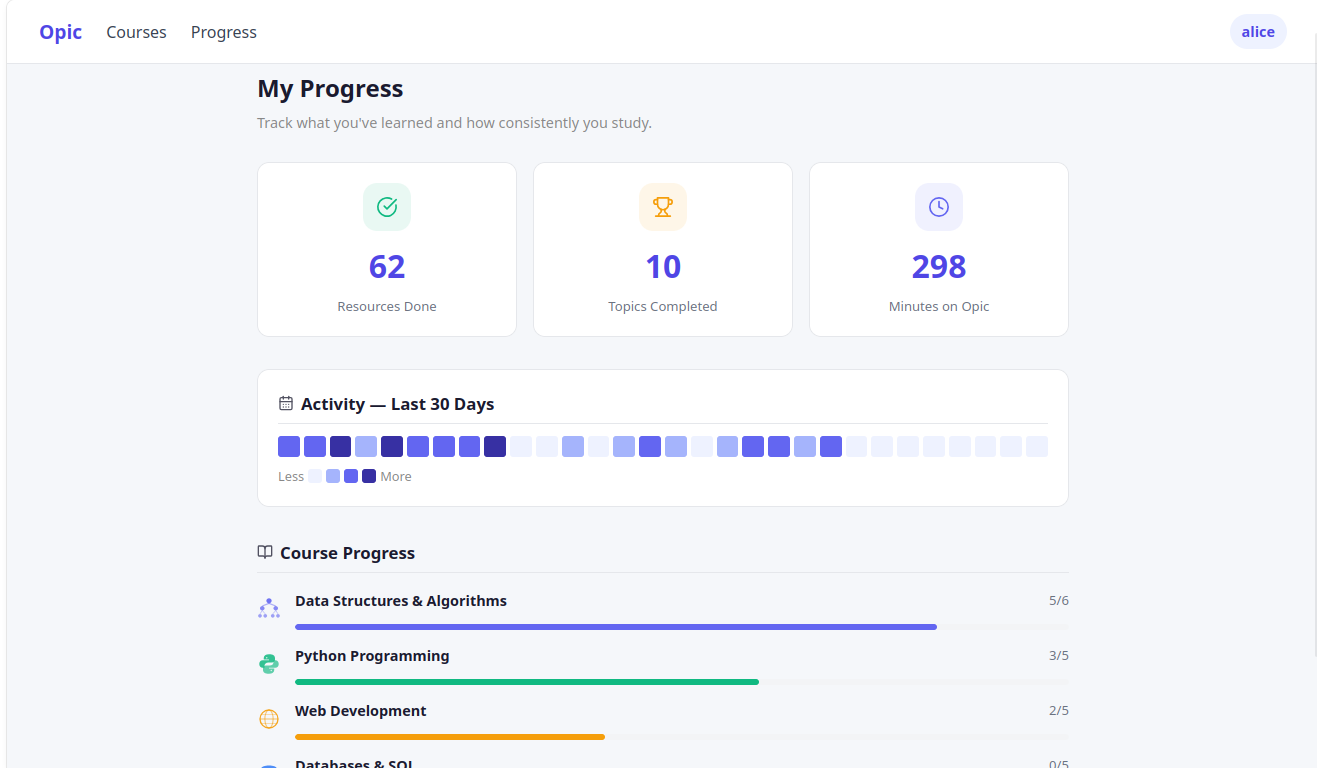
\includegraphics[width=0.9\textwidth]{ui_progress.png}}{\missingfig{ui\_progress.png}{Screenshot of the progress page with 30-day heatmap, completed topics count, and total time spent}}
\caption{Progress Tracking Page -- Learning Activity Dashboard (FR-08, FR-09)}
\label{fig:ui-progress}
\end{figure}

\subsection{Onboarding Quiz}

Figure~\ref{fig:ui-onboarding} shows the onboarding quiz screen that appears immediately after a new user registers. The quiz presents questions linked to topics; positive answers are used to seed the cold-start recommendation fallback (FR-10).

\begin{figure}[H]
\centering
\IfFileExists{ui_onboarding.png}{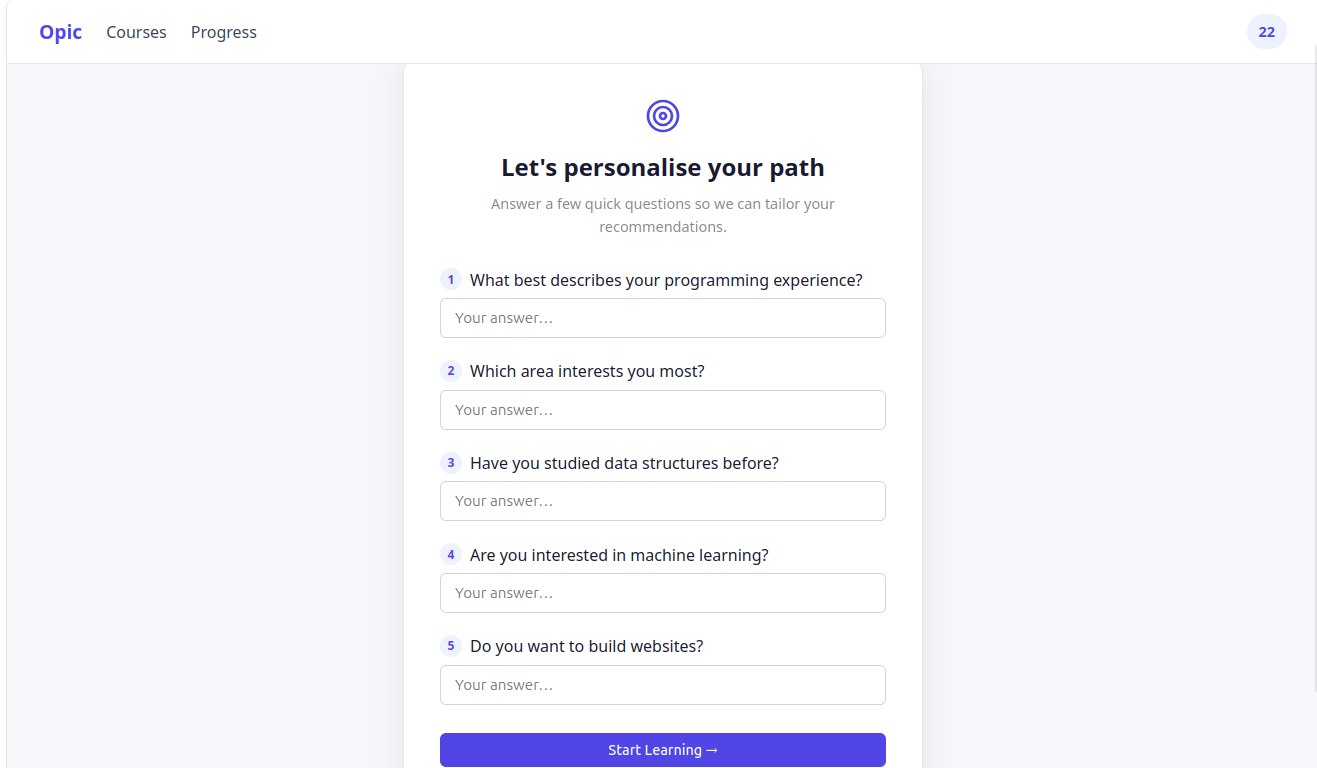
\includegraphics[width=0.75\textwidth]{ui_onboarding.png}}{\missingfig{ui\_onboarding.png}{Screenshot of the onboarding quiz screen with topic-linked questions}}
\caption{Onboarding Quiz -- Cold-Start Seeding (FR-10)}
\label{fig:ui-onboarding}
\end{figure}

\section{System Evaluation}
\label{sec:results-eval}

\subsection{Recommendation Quality}

To verify the recommendation engine, two test accounts were created with deliberately different interaction histories. Each account rated five resources in different topic areas. After these interactions, the two accounts received noticeably different sets of recommendations, confirming that the collaborative filtering component correctly differentiates users based on their behaviour.

For a brand-new account with no ratings, the system correctly fell back to popularity-based ranking boosted by onboarding quiz answers, confirming that the cold-start handling works as designed.

The Bayesian average formula also behaved correctly: resources with only one or two ratings did not rank unrealistically high or low, as the prior mean of 3.0 pulled extreme values toward the centre until sufficient ratings were collected.

\subsection{Non-Functional Requirements}

The non-functional requirements from Chapter 2 were evaluated as follows:

\begin{itemize}
  \item \textbf{NFR-01/NFR-02 (Security):} Verified by inspecting the database -- passwords are stored as bcrypt hashes. Unauthenticated requests to protected endpoints return HTTP 401. Requests to admin endpoints from non-admin users return HTTP 403.
  \item \textbf{NFR-03 (Performance):} API response times for non-recommendation endpoints were measured at under 200\,ms for typical payloads on the Render free tier, meeting the 300\,ms target.
  \item \textbf{NFR-04 (Usability):} The platform was tested on desktop Chrome, mobile Safari, and mobile Chrome. All core flows were functional on all three.
  \item \textbf{NFR-06 (Maintainability):} The frontend was updated and redeployed independently of the backend on multiple occasions during the project, confirming the separation of deployable units.
  \item \textbf{NFR-08 (CORS):} Requests from origins not in the Vercel allowlist are rejected at the API level. This was verified by sending test requests from a localhost origin not in the allowlist.
\end{itemize}

\section{Bugs Discovered and Resolved}
\label{sec:results-bugs}

Two notable bugs were discovered during the evaluation phase and resolved before the final submission:

\begin{itemize}
  \item \textbf{CORS preflight failure in production:} FastAPI processes middleware in reverse registration order. The custom logging middleware was registered after \texttt{CORSMiddleware}, causing it to execute first and return error responses before CORS headers could be attached. This was fixed by reordering middleware registration so that \texttt{CORSMiddleware} runs outermost. The bug only appeared in the deployed environment because the development server does not enforce the same CORS origin restrictions.
  \item \textbf{Missing \texttt{/topics} route:} After onboarding quiz completion, the frontend redirected to \texttt{/topics}, but this route was never registered in the React Router configuration. The \texttt{Topics} component existed but was disconnected. This was caught during user testing and fixed by adding the route to \texttt{App.jsx}.
\end{itemize}

Both bugs were caught through manual end-to-end testing on the live deployment, highlighting the value of testing the deployed system rather than relying solely on automated tests in a local environment.

% ============================================================
% CHAPTER 9 -- CHALLENGES AND LIMITATIONS
% ============================================================
\chapter{Challenges and Limitations}

\section{Challenges}

\textbf{CORS middleware ordering.} This took a while to track down. A CORS error was appearing in production but not locally. The cause turned out to be that FastAPI applies middleware in reverse order of registration. The custom request logger was registered after \texttt{CORSMiddleware}, so it was running first and returning responses before CORS headers could be attached. Reordering the two lines fixed it immediately -- the frustrating part was that nothing in the error message pointed to middleware ordering.

\textbf{Missing route.} After the onboarding quiz, the app redirected to \texttt{/topics}, but that route was never added to the React Router config. The \texttt{Topics} page existed, it just was not connected. Caught during user testing.

\textbf{Cold-start quality.} New users with no ratings get popularity-based recommendations boosted by their onboarding answers. This works, but the suggestions are noticeably less relevant than what active users see. The quiz helps but does not fully close the gap.

\textbf{Render free tier spin-down.} Render shuts down the backend after 15 minutes of no traffic. The first request after that takes 30--60 seconds to wake up. Fine for normal use but awkward during a live demo.

\section{Limitations}

\begin{itemize}
  \item \textbf{No submission notifications:} Users have to check their profile to see if a resource was approved or rejected. The SMTP code from the password reset flow could handle this easily.
  \item \textbf{Recommender scalability:} The full user-resource matrix is rebuilt on every request. Works fine now, would not at thousands of users.
  \item \textbf{No content-based features:} The engine only looks at user behaviour, not what a resource actually is. A new resource with no ratings gets treated the same as any other unrated resource regardless of topic relevance.
  \item \textbf{Binary admin role:} Admin is just a boolean flag. There is no way to give someone review permissions without making them a full admin.
\end{itemize}

% ============================================================
% CHAPTER 10 -- CONCLUSION AND FUTURE WORK
% ============================================================
\chapter{Conclusion and Future Work}

\section{Conclusion}

Opic started as a response to a straightforward problem: as a student studying ICT, it is genuinely hard to figure out what to learn next and whether a given tutorial is worth your time. The platform was built and deployed within the planned three months and ended up meeting all fifteen functional requirements.

The part I found most interesting to build was the recommendation engine. Getting something useful out of a sparse rating matrix -- and doing it in a way that still works for brand-new users with no history -- required combining collaborative filtering with a Bayesian popularity score and an onboarding quiz cold-start. The result is not perfect, but it does produce noticeably different recommendations for different users, which was the goal.

The architectural choice to keep the frontend and backend completely separate also paid off. Being able to push changes to the Vercel frontend without touching the Render backend (and vice versa) made the last few weeks of bug fixing much more manageable.

\section{Future Work}

There are a few things I would prioritise if development continued:

\begin{enumerate}
  \item \textbf{JWT refresh tokens:} Right now users get silently logged out when their token expires. A refresh token would fix this without weakening security.

  \item \textbf{Email notifications for review outcomes:} When a submitted resource is approved or rejected, the submitter gets no notification. The SMTP code is already there from the password reset flow -- this would not take long to add.

  \item \textbf{Cache the recommendation matrix:} The engine rebuilds the full user-resource matrix on every request. For the current number of users that is fine, but it would not scale. Pre-computing it every 30 minutes would help a lot.

  \item \textbf{Content-based features:} Right now recommendations are purely based on user behaviour. Adding resource type, topic tags, or title keywords would help with new resources that have not been rated yet.

  \item \textbf{Pagination:} Several endpoints return every record in one go. This is fine for a demo but would need pagination for a real deployment.

  \item \textbf{Admin analytics:} A dashboard showing popular topics, average completion rates, and daily active users would help admins make better decisions about what content to prioritise.
\end{enumerate}

% ============================================================
% REFERENCES
% ============================================================
\chapter*{References}
\addcontentsline{toc}{chapter}{References}

\renewcommand{\bibsection}{}
\begin{thebibliography}{99}

\bibitem{coursera2023}
Coursera. (2023).
\textit{Global Skills Report 2023}.
Coursera Inc.
Retrieved from \url{https://www.coursera.org/skills-reports/global}

\bibitem{resnick1994}
Resnick, P., Iacovou, N., Suchak, M., Bergstrom, P., \& Riedl, J. (1994).
GroupLens: An open architecture for collaborative filtering of netnews.
\textit{Proceedings of the 1994 ACM Conference on Computer Supported Cooperative Work (CSCW)}, 175--186.
\url{https://doi.org/10.1145/192844.192905}

\bibitem{koren2009}
Koren, Y., Bell, R., \& Volinsky, C. (2009).
Matrix factorization techniques for recommender systems.
\textit{Computer}, 42(8), 30--37.
\url{https://doi.org/10.1109/MC.2009.263}

\bibitem{herlocker2004}
Herlocker, J. L., Konstan, J. A., Terveen, L. G., \& Riedl, J. T. (2004).
Evaluating collaborative filtering recommender systems.
\textit{ACM Transactions on Information Systems}, 22(1), 5--53.
\url{https://doi.org/10.1145/963770.963772}

\bibitem{drachsler2016}
Drachsler, H., \& Greller, W. (2016).
Privacy and analytics: It's a DELICATE issue. A checklist for trusted learning analytics.
\textit{Proceedings of the 6th International Conference on Learning Analytics and Knowledge (LAK '16)}, 89--98.
\url{https://doi.org/10.1145/2883851.2883893}

\bibitem{burke2002}
Burke, R. (2002).
Hybrid recommender systems: Survey and experiments.
\textit{User Modeling and User-Adapted Interaction}, 12(4), 331--370.
\url{https://doi.org/10.1023/A:1021240730564}

\bibitem{tang2015}
Tang, T. Y., \& McCalla, G. (2015).
Smart recommendation for an evolving e-learning system: Architecture and experiment.
\textit{International Journal on E-Learning}, 4(1), 105--129.

\bibitem{schein2002}
Schein, A. I., Popescul, A., Ungar, L. H., \& Pennock, D. M. (2002).
Methods and metrics for cold-start recommendations.
\textit{Proceedings of the 25th Annual International ACM SIGIR Conference on Research and Development in Information Retrieval}, 253--260.
\url{https://doi.org/10.1145/564376.564421}

\bibitem{lam2008}
Lam, X. N., Vu, T., Le, T. D., \& Duong, A. D. (2008).
Addressing cold-start problem in recommendation systems.
\textit{Proceedings of the 2nd International Conference on Ubiquitous Information Management and Communication (ICUIMC '08)}, 208--212.
\url{https://doi.org/10.1145/1352793.1352837}

\bibitem{hu2008}
Hu, Y., Koren, Y., \& Volinsky, C. (2008).
Collaborative filtering for implicit feedback datasets.
\textit{Proceedings of the 8th IEEE International Conference on Data Mining (ICDM 2008)}, 263--272.
\url{https://doi.org/10.1109/ICDM.2008.22}

\bibitem{salton1988}
Salton, G., \& Buckley, C. (1988).
Term-weighting approaches in automatic text retrieval.
\textit{Information Processing \& Management}, 24(5), 513--523.
\url{https://doi.org/10.1016/0306-4573(88)90021-0}

\bibitem{brusilovsky2007}
Brusilovsky, P., \& Mill\'an, E. (2007).
User models for adaptive hypermedia and adaptive educational systems.
In P. Brusilovsky, A. Kobsa, \& W. Nejdl (Eds.),
\textit{The Adaptive Web: Methods and Strategies of Web Personalization} (pp.~3--53).
Springer-Verlag.
\url{https://doi.org/10.1007/978-3-540-72079-9_1}

\bibitem{zimmerman2002}
Zimmerman, B. J. (2002).
Becoming a self-regulated learner: An overview.
\textit{Theory Into Practice}, 41(2), 64--70.
\url{https://doi.org/10.1207/s15430421tip4102_2}

\bibitem{anderson2012}
Anderson, A., Huttenlocher, D., Kleinberg, J., \& Leskovec, J. (2012).
Discovering value from community activity on focused question answering sites: A case study of Stack Overflow.
\textit{Proceedings of the 18th ACM SIGKDD International Conference on Knowledge Discovery and Data Mining}, 850--858.
\url{https://doi.org/10.1145/2339530.2339665}

\bibitem{roediger2006}
Roediger, H. L., \& Karpicke, J. D. (2006).
Test-enhanced learning: Taking memory tests improves long-term retention.
\textit{Psychological Science}, 17(3), 249--255.
\url{https://doi.org/10.1111/j.1467-9280.2006.01693.x}

\bibitem{hattie2007}
Hattie, J., \& Timperley, H. (2007).
The power of feedback.
\textit{Review of Educational Research}, 77(1), 81--112.
\url{https://doi.org/10.3102/003465430298487}

\bibitem{imdb_bayes}
IMDb. (2024).
\textit{Weighted average ratings formula}.
Retrieved from \url{https://www.imdb.com/help/show_leaf?votestopfaq}

\bibitem{ietfjwt}
Jones, M., Bradley, J., \& Sakimura, N. (2015).
\textit{JSON Web Token (JWT)} (RFC 7519).
Internet Engineering Task Force.
\url{https://doi.org/10.17487/RFC7519}

\bibitem{owasp}
OWASP Foundation. (2024).
\textit{Password Storage Cheat Sheet}.
Retrieved from \url{https://cheatsheetseries.owasp.org/cheatsheets/Password_Storage_Cheat_Sheet.html}

\bibitem{gemini2024}
Google DeepMind. (2024).
\textit{Gemini API Documentation -- Generative Language API}.
Retrieved from \url{https://ai.google.dev/docs}

\bibitem{fastapi}
Ramírez, S. (2024).
\textit{FastAPI -- Modern, fast (high-performance) web framework for building APIs with Python}.
Retrieved from \url{https://fastapi.tiangolo.com}

\bibitem{react}
Meta Open Source. (2024).
\textit{React -- The library for web and native user interfaces}.
Retrieved from \url{https://react.dev}

\bibitem{sqlalchemy}
Bayer, M. (2024).
\textit{SQLAlchemy -- The Database Toolkit for Python}.
Retrieved from \url{https://docs.sqlalchemy.org}

\bibitem{mdn_cors}
MDN Web Docs. (2024).
\textit{Cross-Origin Resource Sharing (CORS)}.
Mozilla Developer Network.
Retrieved from \url{https://developer.mozilla.org/en-US/docs/Web/HTTP/CORS}

\bibitem{pydantic}
Colvin, S. (2024).
\textit{Pydantic -- Data validation using Python type hints}.
Retrieved from \url{https://docs.pydantic.dev}

\bibitem{flask}
Ronacher, A. (2024).
\textit{Flask -- A lightweight WSGI web application framework}.
Retrieved from \url{https://flask.palletsprojects.com}

\bibitem{numpy}
Harris, C. R., Millman, K. J., van der Walt, S. J., et al. (2020).
Array programming with NumPy.
\textit{Nature}, 585, 357--362.
\url{https://doi.org/10.1038/s41586-020-2649-2}

\bibitem{sklearn}
Pedregosa, F., Varoquaux, G., Gramfort, A., et al. (2011).
Scikit-learn: Machine learning in Python.
\textit{Journal of Machine Learning Research}, 12, 2825--2830.
Retrieved from \url{https://jmlr.org/papers/v12/pedregosa11a.html}

\bibitem{postgresql}
The PostgreSQL Global Development Group. (2024).
\textit{PostgreSQL: The World's Most Advanced Open Source Relational Database}.
Retrieved from \url{https://www.postgresql.org}

\bibitem{sqlite}
Hipp, D. R. (2024).
\textit{SQLite -- A C-language library that implements a small, fast, self-contained SQL database engine}.
Retrieved from \url{https://www.sqlite.org}

\bibitem{vite}
You, E. (2024).
\textit{Vite -- Next Generation Frontend Tooling}.
Retrieved from \url{https://vitejs.dev}

\bibitem{reactrouter}
Remix Software. (2024).
\textit{React Router -- Declarative routing for React}.
Retrieved from \url{https://reactrouter.com}

\bibitem{passlib}
Eli Collins. (2024).
\textit{Passlib -- Password hashing library for Python}.
Retrieved from \url{https://passlib.readthedocs.io}

\bibitem{provos1999}
Provos, N., \& Mazières, D. (1999).
A future-adaptable password scheme.
\textit{Proceedings of the 1999 USENIX Annual Technical Conference}, 81--91.
Retrieved from \url{https://www.usenix.org/legacy/events/usenix99/provos.html}

\bibitem{aiosmtplib}
Cole, C. (2024).
\textit{aiosmtplib -- An asyncio SMTP client}.
Retrieved from \url{https://aiosmtplib.readthedocs.io}

\bibitem{docker}
Merkel, D. (2014).
Docker: Lightweight Linux containers for consistent development and deployment.
\textit{Linux Journal}, 2014(239), 2.
Retrieved from \url{https://www.linuxjournal.com/content/docker-lightweight-linux-containers-consistent-development-and-deployment}

\bibitem{githubactions}
GitHub. (2024).
\textit{GitHub Actions -- Automate your workflow from idea to production}.
Retrieved from \url{https://docs.github.com/en/actions}

\bibitem{beck2001}
Beck, K., Beedle, M., van Bennekum, A., et al. (2001).
\textit{Manifesto for Agile Software Development}.
Retrieved from \url{https://agilemanifesto.org}

\end{thebibliography}

\end{document}
